\documentclass[
  man,
  floatsintext,
  longtable,
  nolmodern,
  notxfonts,
  notimes,
  colorlinks=true,linkcolor=blue,citecolor=blue,urlcolor=blue]{apa7}

\usepackage{amsmath}
\usepackage{amssymb}




\RequirePackage{longtable}
\RequirePackage{threeparttablex}

\makeatletter
\renewcommand{\paragraph}{\@startsection{paragraph}{4}{\parindent}%
	{0\baselineskip \@plus 0.2ex \@minus 0.2ex}%
	{-.5em}%
	{\normalfont\normalsize\bfseries\typesectitle}}

\renewcommand{\subparagraph}[1]{\@startsection{subparagraph}{5}{0.5em}%
	{0\baselineskip \@plus 0.2ex \@minus 0.2ex}%
	{-\z@\relax}%
	{\normalfont\normalsize\bfseries\itshape\hspace{\parindent}{#1}\textit{\addperi}}{\relax}}
\makeatother




\usepackage{longtable, booktabs, multirow, multicol, colortbl, hhline, caption, array, float, xpatch}
\usepackage{subcaption}


\renewcommand\thesubfigure{\Alph{subfigure}}
\setcounter{topnumber}{2}
\setcounter{bottomnumber}{2}
\setcounter{totalnumber}{4}
\renewcommand{\topfraction}{0.85}
\renewcommand{\bottomfraction}{0.85}
\renewcommand{\textfraction}{0.15}
\renewcommand{\floatpagefraction}{0.7}

\usepackage{tcolorbox}
\tcbuselibrary{listings,theorems, breakable, skins}
\usepackage{fontawesome5}

\definecolor{quarto-callout-color}{HTML}{909090}
\definecolor{quarto-callout-note-color}{HTML}{0758E5}
\definecolor{quarto-callout-important-color}{HTML}{CC1914}
\definecolor{quarto-callout-warning-color}{HTML}{EB9113}
\definecolor{quarto-callout-tip-color}{HTML}{00A047}
\definecolor{quarto-callout-caution-color}{HTML}{FC5300}
\definecolor{quarto-callout-color-frame}{HTML}{ACACAC}
\definecolor{quarto-callout-note-color-frame}{HTML}{4582EC}
\definecolor{quarto-callout-important-color-frame}{HTML}{D9534F}
\definecolor{quarto-callout-warning-color-frame}{HTML}{F0AD4E}
\definecolor{quarto-callout-tip-color-frame}{HTML}{02B875}
\definecolor{quarto-callout-caution-color-frame}{HTML}{FD7E14}

%\newlength\Oldarrayrulewidth
%\newlength\Oldtabcolsep


\usepackage{hyperref}




\providecommand{\tightlist}{%
  \setlength{\itemsep}{0pt}\setlength{\parskip}{0pt}}
\usepackage{longtable,booktabs,array}
\usepackage{calc} % for calculating minipage widths
% Correct order of tables after \paragraph or \subparagraph
\usepackage{etoolbox}
\makeatletter
\patchcmd\longtable{\par}{\if@noskipsec\mbox{}\fi\par}{}{}
\makeatother
% Allow footnotes in longtable head/foot
\IfFileExists{footnotehyper.sty}{\usepackage{footnotehyper}}{\usepackage{footnote}}
\makesavenoteenv{longtable}

\usepackage{graphicx}
\makeatletter
\newsavebox\pandoc@box
\newcommand*\pandocbounded[1]{% scales image to fit in text height/width
  \sbox\pandoc@box{#1}%
  \Gscale@div\@tempa{\textheight}{\dimexpr\ht\pandoc@box+\dp\pandoc@box\relax}%
  \Gscale@div\@tempb{\linewidth}{\wd\pandoc@box}%
  \ifdim\@tempb\p@<\@tempa\p@\let\@tempa\@tempb\fi% select the smaller of both
  \ifdim\@tempa\p@<\p@\scalebox{\@tempa}{\usebox\pandoc@box}%
  \else\usebox{\pandoc@box}%
  \fi%
}
% Set default figure placement to htbp
\def\fps@figure{htbp}
\makeatother


% definitions for citeproc citations
\NewDocumentCommand\citeproctext{}{}
\NewDocumentCommand\citeproc{mm}{%
  \begingroup\def\citeproctext{#2}\cite{#1}\endgroup}
\makeatletter
 % allow citations to break across lines
 \let\@cite@ofmt\@firstofone
 % avoid brackets around text for \cite:
 \def\@biblabel#1{}
 \def\@cite#1#2{{#1\if@tempswa , #2\fi}}
\makeatother
\newlength{\cslhangindent}
\setlength{\cslhangindent}{1.5em}
\newlength{\csllabelwidth}
\setlength{\csllabelwidth}{3em}
\newenvironment{CSLReferences}[2] % #1 hanging-indent, #2 entry-spacing
 {\begin{list}{}{%
  \setlength{\itemindent}{0pt}
  \setlength{\leftmargin}{0pt}
  \setlength{\parsep}{0pt}
  % turn on hanging indent if param 1 is 1
  \ifodd #1
   \setlength{\leftmargin}{\cslhangindent}
   \setlength{\itemindent}{-1\cslhangindent}
  \fi
  % set entry spacing
  \setlength{\itemsep}{#2\baselineskip}}}
 {\end{list}}
\usepackage{calc}
\newcommand{\CSLBlock}[1]{\hfill\break\parbox[t]{\linewidth}{\strut\ignorespaces#1\strut}}
\newcommand{\CSLLeftMargin}[1]{\parbox[t]{\csllabelwidth}{\strut#1\strut}}
\newcommand{\CSLRightInline}[1]{\parbox[t]{\linewidth - \csllabelwidth}{\strut#1\strut}}
\newcommand{\CSLIndent}[1]{\hspace{\cslhangindent}#1}


\usepackage[nolongtablepatch]{lineno}
\linenumbers



\usepackage{newtx}

\defaultfontfeatures{Scale=MatchLowercase}
\defaultfontfeatures[\rmfamily]{Ligatures=TeX,Scale=1}





\title{Negative Perceptions of Outsourcing to Artificial Intelligence}


\shorttitle{Outsourcing to AI}


\usepackage{etoolbox}








\authorsnames{Scott Claessens,Pierce Veitch,Jim A.C. Everett}





\affiliation{
{School of Psychology, University of Kent}}




\leftheader{Claessens, Veitch and Everett}



\abstract{As artificial intelligence (AI) tools become increasingly
integrated into daily life, people are beginning to outsource not only
professional tasks but also socio-relational ones. Large language models
like ChatGPT can generate wedding vows, speeches, and personal messages,
raising questions about how individuals who use AI for such tasks are
perceived by others. In this paper, we conduct five pre-registered
studies with British participants (N = 3,649) to understand how people
view those who outsource tasks to AI, and how this depends on how
socio-relational the task is, whether AI is used as a tool or fully
delegated to, and the acknowledgment of the AI use. We find negative
perceptions of outsourcing, particularly for socio-relational tasks. We
show that outsourcing makes us think more negatively about not only the
person and their motivations, but also the outsourced work itself.
Moreover, we provide insight into why this occurs: the reduced effort
from outsourcing socio-relational tasks to AI signals that the output is
less authentically one's own and that the person cares less about the
task. Our research highlights the way that AI use shapes our perceptions
of people, raising key philosophical questions about efficiency,
authenticity, and social ties in a world filled with AI-mediated
interactions.  \section{Significance Statement} \noindent People form
negative impressions of individuals who use artificial intelligence
tools to complete tasks for them, especially interpersonal tasks like
writing love letters or apology notes. This occurs even when they use AI
as a tool instead of a replacement, are honest about it, and use AI
because they care about doing the task well. We show that doing
something oneself, even if AI could do it quicker and easier, signals
that one is authentic and cares about the task. Our results highlight
that people do not only care about whether something is done, but how it
is done too. }

\keywords{artificial intelligence, person
perception, outsourcing, effort, trust}

\authornote{\par{\addORCIDlink{Scott
Claessens}{0000-0002-3562-6981}}\par{\addORCIDlink{Pierce
Veitch}{0009-0005-3364-7470}}\par{\addORCIDlink{Jim A.C.
Everett}{0000-0003-2801-5426}} 
\par{ }
\par{This pre-print is currently not yet peer-reviewed, and may differ
from the final version. Word count = 9119 words.      Author roles were
classified using the Contributor Role Taxonomy (CRediT;
https://credit.niso.org/) as follows:  Scott
Claessens:   conceptualization, data curation, formal
analysis, investigation, methodology, visualization, writing, editing; Pierce
Veitch:   formal analysis, methodology, editing; Jim A.C.
Everett:   conceptualization, funding
acquisition, methodology, supervision, editing}
\par{Correspondence concerning this article should be addressed to Jim
A.C. Everett, School of Psychology, University of Kent, Keynes
College, Canterbury CT2
7NP, UK, Email: \href{mailto:j.a.c.everett@kent.ac.uk}{j.a.c.everett@kent.ac.uk}}
}

\makeatletter
\let\endoldlt\endlongtable
\def\endlongtable{
\hline
\endoldlt
}
\makeatother

\urlstyle{same}



\usepackage{booktabs}
\usepackage{longtable}
\usepackage{array}
\usepackage{multirow}
\usepackage{wrapfig}
\usepackage{float}
\usepackage{colortbl}
\usepackage{pdflscape}
\usepackage{tabu}
\usepackage{threeparttable}
\usepackage{threeparttablex}
\usepackage[normalem]{ulem}
\usepackage{makecell}
\usepackage{xcolor}
\nolinenumbers
\makeatletter
\@ifpackageloaded{float}{}{\usepackage{float}}
\floatstyle{plain}
\@ifundefined{c@chapter}{\newfloat{suppfig}{h}{losuppfig}}{\newfloat{suppfig}{h}{losuppfig}[chapter]}
\floatname{suppfig}{Supplementary Figure}
\newcommand*\listofsuppfigs{\listof{suppfig}{List of Supplementary Figures}}
\makeatother
\makeatletter
\@ifpackageloaded{float}{}{\usepackage{float}}
\floatstyle{plain}
\@ifundefined{c@chapter}{\newfloat{supptbl}{h}{losupptbl}}{\newfloat{supptbl}{h}{losupptbl}[chapter]}
\floatname{supptbl}{Supplementary Table}
\floatstyle{plaintop}
\restylefloat{supptbl}
\newcommand*\listofsupptbls{\listof{supptbl}{List of Supplementary Tables}}
\makeatother
\makeatletter
\@ifpackageloaded{caption}{}{\usepackage{caption}}
\AtBeginDocument{%
\ifdefined\contentsname
  \renewcommand*\contentsname{Table of contents}
\else
  \newcommand\contentsname{Table of contents}
\fi
\ifdefined\listfigurename
  \renewcommand*\listfigurename{List of Figures}
\else
  \newcommand\listfigurename{List of Figures}
\fi
\ifdefined\listtablename
  \renewcommand*\listtablename{List of Tables}
\else
  \newcommand\listtablename{List of Tables}
\fi
\ifdefined\figurename
  \renewcommand*\figurename{Figure}
\else
  \newcommand\figurename{Figure}
\fi
\ifdefined\tablename
  \renewcommand*\tablename{Table}
\else
  \newcommand\tablename{Table}
\fi
}
\@ifpackageloaded{float}{}{\usepackage{float}}
\floatstyle{ruled}
\@ifundefined{c@chapter}{\newfloat{codelisting}{h}{lop}}{\newfloat{codelisting}{h}{lop}[chapter]}
\floatname{codelisting}{Listing}
\newcommand*\listoflistings{\listof{codelisting}{List of Listings}}
\makeatother
\makeatletter
\usepackage{pdflscape}
\makeatother
\makeatletter
\makeatother
\makeatletter
\@ifpackageloaded{caption}{}{\usepackage{caption}}
\@ifpackageloaded{subcaption}{}{\usepackage{subcaption}}
\makeatother

% From https://tex.stackexchange.com/a/645996/211326
%%% apa7 doesn't want to add appendix section titles in the toc
%%% let's make it do it
\makeatletter
\xpatchcmd{\appendix}
  {\par}
  {\addcontentsline{toc}{section}{\@currentlabelname}\par}
  {}{}
\makeatother

%% Disable longtable counter
%% https://tex.stackexchange.com/a/248395/211326

\usepackage{etoolbox}

\makeatletter
\patchcmd{\LT@caption}
  {\bgroup}
  {\bgroup\global\LTpatch@captiontrue}
  {}{}
\patchcmd{\longtable}
  {\par}
  {\par\global\LTpatch@captionfalse}
  {}{}
\apptocmd{\endlongtable}
  {\ifLTpatch@caption\else\addtocounter{table}{-1}\fi}
  {}{}
\newif\ifLTpatch@caption
\makeatother

\begin{document}

\maketitle



\setcounter{secnumdepth}{-\maxdimen} % remove section numbering

\setlength\LTleft{0pt}

\resetlinenumber[1]



\linenumbers

The widespread release of generative AI language models has transformed
daily life, offering the potential to perform a variety of tasks more
efficiently and, in some cases, with greater effectiveness than by doing
them oneself. But as AI becomes more widely available, people are not
only using it to assist them with things like preparing dinner recipes,
writing data analysis code, and planning daily schedules. Increasingly,
AI might be used beyond routine or technical domains to instead assist
in tasks that are more socio-relational in nature, like writing wedding
vows, apology notes, and love letters. Anecdotal evidence suggests that
not only is AI-outsourcing of this kind already happening, but that it
potentially has serious effects on how we judge others. In a recent
Reddit post, a disgruntled newlywed tells the story of her husband using
ChatGPT to write his wedding vows, expressing her discomfort with
outsourcing something to AI that, to her, is deeply meaningful and a
reflection of their love for one another
(\citeproc{ref-miramar0}{miramar0, 2024}). Other reports describe
people's negative reactions when they learn that their romantic partner
used ChatGPT to write them an apology note
(\citeproc{ref-Tait2024}{Tait, 2024}) or even to break up with them
(\citeproc{ref-Anderson2025}{Anderson, 2025}). Outsourcing tasks --
especially socio-relational ones -- to AI tools may be efficient, but
could have negative consequences for person perception.

There is nothing new, in principle, about outsourcing tasks. For
hundreds of years, personal assistants have organised daily schedules,
recipe-books have provided meal plans, and guidebooks have created
travel itineraries. In the socio-relational domain, ghostwriters have
long-existed, and the internet is abound with professional paid services
for writing wedding vows and personal speeches. AI merely supercharges
what is an ancient human impulse: the push to reduce mental energy by
outsourcing parts of our work onto people, books, tools, or systems. But
even if outsourcing is an old phenomenon, the rapid shift in
availability and use of AI models has fundamentally changed the ease
with which people can outsource work, what kinds of tasks they can
outsource, and the way in which they can outsource. These new
developments in society mean that even as an old phenomenon in new
clothes, there is much we still need to know about outsourcing.

First, we need to know how people who outsource tasks to AI are
perceived. We know that people are increasingly using large language
models (LLMs) for a wide variety of tasks
(\citeproc{ref-UKGov2024}{Department for Science, Innovation \&
Technology, 2024}). Due to their ubiquity, perhaps outsourcing to LLMs
might not lead to negative perceptions? We are sceptical. We know that
people dislike it when others ``free ride'' or reduce effort while
benefiting from collective resources (e.g.
\citeproc{ref-Cubitt2011}{Cubitt et al., 2011};
\citeproc{ref-Kerr1983}{Kerr, 1983}) and that people's outputs are
perceived as more valuable the more effort was ostensibly put into them
(\citeproc{ref-Kruger2004}{Kruger et al., 2004}). Moreover, exertion of
effort is deemed morally admirable and is rewarded, even in situations
where effort does not directly generate additional product, quality, or
economic value, suggesting that effort itself is moralised
(\citeproc{ref-Celniker2023}{Celniker et al., 2023}). Given this, even
if AI tools are widely available and pitched as improving efficiency,
the core social psychological processes are likely to remain: someone is
expending less effort to achieve a task, and people value effort.
Indeed, some work shows that describing someone as using AI for a
relational task led to the perception they expended less effort and were
less satisfied with their relationship (\citeproc{ref-Liu2024}{Liu et
al., 2024}) and other unpublished work looking at perceptions of people
using AI to complete academic assignments finds that using AI leads to
more negative perceptions of moral character and suitability as a
partner (\citeproc{ref-Roth2025}{Roth \& Tissot, 2025}).

Second, we need to know whether the \emph{type} of task that people are
outsourcing matters. One might expect outsourcing to be perceived
negatively regardless of the type of task being outsourced -- if effort
is generally moralised, then the domain in which it is expended (or not)
should have little impact. However, there are reasons to expect
differences between social tasks like writing vows and non-social tasks
like writing computer code. We know that different norms, standards, and
expectations can be applied to social and non-social tasks and exchanges
(e.g. \citeproc{ref-Fiske1992}{A. P. Fiske, 1992};
\citeproc{ref-Heider1958}{Heider, 1958}; \citeproc{ref-Malle2022}{Malle,
2022}). Moreover, from a philosophical perspective, it often matters not
only \emph{whether} something is done, but \emph{how} it is done
(\citeproc{ref-Aristotle2009}{Aristotle, 2009};
\citeproc{ref-Hursthouse2023}{Hursthouse \& Pettigrove, 2023};
\citeproc{ref-Stohr2006}{Stohr, 2006}). An apology is not just about
hearing someone say ``I am sorry'', but seeing genuine regret; a love
letter is not just about hearing someone say ``I love you'', but seeing
depth of emotion; and a bereavement letter is not just about hearing
someone say ``I am sorry for your loss'', but seeing an understanding
for the powerful human experience of loss. There is, perhaps especially
for social tasks, value not only in the outcome of doing something, but
the \emph{process} too (\citeproc{ref-Goodman2010}{Goodman, 2010}). To
understand any potential negative effects of outsourcing to AI, we must
therefore look at a broad range of non-social and social tasks, rather
than draw broad conclusions based on a few use cases.

Third, we need to know how different ways of outsourcing to AI influence
negative perceptions. Someone who ``fully'' outsources a task to AI by
simply giving it a prompt and copying the output word-for-word might be
perceived very differently to someone who gives the AI a prompt, revises
the work accordingly, and finishes it themselves -- using AI as a
\emph{collaborative tool}, rather than as a replacement. Similarly,
someone could deceive others about their use of AI or be perfectly
honest about it. While it seems reasonable to assume that ``fully''
outsourcing would be perceived worse than using AI as a tool, and that
not acknowledging AI use would be perceived worse than being honest
about it, it remains unclear how much this reduces negative perceptions:
if someone uses AI in the ``best'' way, by using it as a collaborative
tool and being open about this use, would they still suffer negative
social consequences from doing so?

Fourth, we need to know how outsourcing to AI, in different kinds of
tasks and in different ways, may shape different \emph{kinds} of social
perceptions. People can judge others on separate dimensions of warmth
and competence (e.g. \citeproc{ref-Abele2021}{Abele et al., 2021};
\citeproc{ref-Fiske2007}{S. T. Fiske et al., 2007}) as well as on
dimensions of morality and trustworthiness
(\citeproc{ref-Goodwin2014}{Goodwin et al., 2014}). It remains unclear
how outsourcing to AI might lead to differential character judgments
across these different dimensions.

Fifth, we need to understand \emph{why} outsourcing to AI, and therefore
expending less effort, might have these effects. Previous work has
focused on how expending less effort leads to negative perceptions of
others (\citeproc{ref-Celniker2023}{Celniker et al., 2023}). But this
raises the question of \emph{why} effort is seen as important and what
exactly it is signalling to others, beyond one's general cooperative
intent. It is possible that outsourcing leads to negative perceptions
because the lack of effort spent on the task signals something more
fundamental about how authentic one is and how much one cares about the
task: when someone chooses to outsource a love letter to an AI, they
might be seen as valuing that love letter and what it represents less.
It could be this second-step order of perceptions that is the key driver
of negative perceptions, especially for socio-relational tasks.

\subsection*{Present Research}\label{present-research}

In this paper, we build on classic social psychological work on
character inferences from reduced effort to understand how people view
others who outsource different kinds of tasks, in different ways, for
different reasons, to AI. Across five pre-registered experiments with
British participants, we seek not only to understand how reduced effort
through AI-outsourcing might shape perceptions of others, but also to
understand in more depth \emph{why} it is that reduced effort has the
effect that it does.

In our initial pilot studies to motivate this work, we found that people
who outsource a range of tasks to AI or another person are perceived
more negatively than people who complete the tasks by themselves (see
Supplementary Materials). In Study 1, we look at the effects of task
type, AI use, and honesty. We explore how people perceive others who
outsource different kinds of tasks with different levels of social
relevance (e.g., from daily schedules, computer code and dinner recipes
to wedding vows, apology letters, or bereavement cards), manipulating
whether people use AI as a collaborative tool or ``fully'' outsource to
AI and whether they are honest or deceptive about their use of AI. After
turning to look at perceptions of both outsourcers and the outsourced
work in Study 2, in Studies 3-5 we probe why outsourcing may have
negative effects on how we evaluate others. In Study 3, we test
potential mechanisms of perceived effort and authenticity by looking at
how people evaluate others who either spend a lot or little time
crafting the AI prompts, and who either outsource to a generic or
personalised AI. In Study 4, we test the potential mechanism of
perceived importance in the task by manipulating people's reasons for
using AI -- either because they wanted to save time or because they
cared about the task and thought that AI would improve their work.
Finally, in Study 5, we bring these different potential mechanisms
together to explore the different pathways that influence the
relationship between outsourcing and negative perceptions, focusing on
perceived effort, authenticity, and care in the task.

\newpage

\section*{Study 1}\label{study-1}

\subsection*{Methods}\label{methods}

\subsubsection*{Ethical Approval}\label{ethical-approval}

Ethical approval was granted for all studies in this paper by the
REDACTED Psychology Research Ethics Panel. Participants in all studies
provided informed consent and were debriefed after the study.

\subsubsection*{Participants}\label{participants}

We conducted a power simulation to determine our target sample size. The
simulation suggested that a sample size of 150 participants per
condition (overall \emph{n} = 750 for five conditions) would be required
to detect a small difference between conditions (Cohen's \emph{d} ≈
0.20) with above 80\% power.

We recruited a convenience sample of 800 participants from the United
Kingdom through the online platform Prolific
(\url{https://www.prolific.com/}). After excluding participants who
failed our pre-treatment attention check, we were left with a final
sample of 762 participants (438 female; 316 male; 4 non-binary / third
gender; 4 undisclosed gender; mean age = 42.16 years). 78\% of these
participants reported having used ChatGPT before.

\subsubsection*{Design}\label{design}

We used a ``control plus 2x2'' between-subjects design. Participants
were randomly allocated to either the control condition, in which people
in the scenarios complete the tasks themselves, or one of four
experimental conditions, in which people in the scenarios use AI to
complete the tasks. In the experimental conditions, we manipulated
whether people in the scenarios used AI as a collaborative tool or
``fully'' outsourced to AI, and whether people were honest or deceptive
about their use of AI. This resulted in five conditions overall:
(\emph{i}) the control condition, (\emph{ii}) the tool-honest condition,
(\emph{iii}) the tool-deception condition, (\emph{iv}) the full-honest
condition, and (\emph{v}) the full-deception condition.

\subsubsection*{Procedure}\label{procedure}

We presented participants with six scenarios. Each scenario described a
person completing a task, such as writing computer code or writing a
love letter. The six tasks were randomly drawn from a larger set of 16
tasks (see Supplementary Table~\ref{supptbl-tasks} for the full list of
tasks). For each scenario, we first told participants:

\begin{itemize}
\tightlist
\item
  \emph{Control condition}: ``In order to complete this task, {[}the
  person{]} works on it by themselves from start to finish.''
\item
  \emph{Tool outsourcing conditions}: ``In order to complete this task,
  {[}the person{]} uses the AI tool ChatGPT. They ask ChatGPT to provide
  ideas, inspiration, and feedback, but they edit and rewrite the
  suggestions and finish the task themselves.''
\item
  \emph{Full outsourcing conditions}: ``In order to complete this task,
  {[}the person{]} uses the AI tool ChatGPT. They copy ChatGPT's output
  word-for-word, rather than doing it themselves.''
\end{itemize}

We then told participants in the experimental conditions:

\begin{itemize}
\tightlist
\item
  \emph{Honest conditions}: ``After completing the task, {[}the
  person{]} is asked how they came up with their ideas. {[}The person{]}
  acknowledges that they used ChatGPT as a tool / got ChatGPT to do the
  task for them.''
\item
  \emph{Deception conditions}: ``After completing the task, {[}the
  person{]} is asked how they came up with their ideas. {[}The person{]}
  does not acknowledge that they used ChatGPT as a tool / got ChatGPT to
  do the task for them.''
\end{itemize}

We then asked participants how well each of the following words
described the person in the scenario: competent, warm, moral, lazy, and
trustworthy. Participants answered these questions on 7-point Likert
scales, ranging from ``does not describe {[}the person{]} well'' to
``describes {[}the person{]} extremely well''.

After the six scenarios, we asked participants several questions about
the AI tool ChatGPT, including their familiarity with ChatGPT, whether
they had used ChatGPT before, how frequently they used ChatGPT, and how
trustworthy they thought ChatGPT was.

\subsubsection*{Pre-registration}\label{pre-registration}

We pre-registered the study on the Open Science Framework
(\url{https://osf.io/xhmzk/?view_only=a4da193574d7410ba4d2aa3945a28b05}).

\subsubsection*{Statistical Analysis}\label{statistical-analysis}

We fitted Bayesian multivariate multilevel cumulative-link ordinal
models to the data using the \emph{brms} R package
(\citeproc{ref-Burkner2017}{Bürkner, 2017}). We modelled each character
evaluation -- competence, warmth, morality, laziness, and
trustworthiness -- as a separate response variable and included fixed
effects for conditions, varying intercepts for participants, and varying
intercepts and slopes for tasks. We used regularising priors for all
parameters to impose conservatism on parameter estimates. All models
converged normally (\(\hat{R}\) ≤ 1.01).

\subsubsection*{Transparency and
Openness}\label{transparency-and-openness}

For all studies in this paper, we report how we determined our sample
size, all data exclusions, all manipulations, and all measures in the
studies. All studies were pre-registered. Analyses for all studies were
conducted in R v4.4.2 (\citeproc{ref-RCoreTeam}{R Core Team, 2022}).
Visualisations were produced using the \emph{ggplot2} and
\emph{patchwork} packages (\citeproc{ref-Pedersen2025}{Pedersen, 2025};
\citeproc{ref-Wickham2016}{Wickham, 2016}). The manuscript was
reproducibly generated using the \emph{targets} package
(\citeproc{ref-Landau2021}{Landau, 2021}) and \emph{quarto}
(\citeproc{ref-Allaire2024}{Allaire et al., 2024}). All data and code to
reproduce the analyses and figures in this paper can be found here:
\url{https://osf.io/xhmzk/?view_only=a4da193574d7410ba4d2aa3945a28b05}

\subsection*{Results}\label{results}

We first looked at the overall results averaging over tasks. Across all
five character evaluations, we found that fully outsourcing to AI (i.e.,
copying the AI output verbatim) was perceived more negatively than using
AI as a collaborative tool (Figure~\ref{fig-treatments-study1};
Table~\ref{tbl-treatment-diffs-study1}). By contrast, we found that
deception about AI usage had specific negative effects on perceptions of
morality and trustworthiness: people who did not acknowledge their use
of AI were perceived as less moral and less trustworthy. We did not find
any interaction effects between full outsourcing and deception.

\begin{figure}[!htbp]

{\caption{{Overall Character Evaluations in Study
1}{\label{fig-treatments-study1}}}}

\begin{center}
\pandocbounded{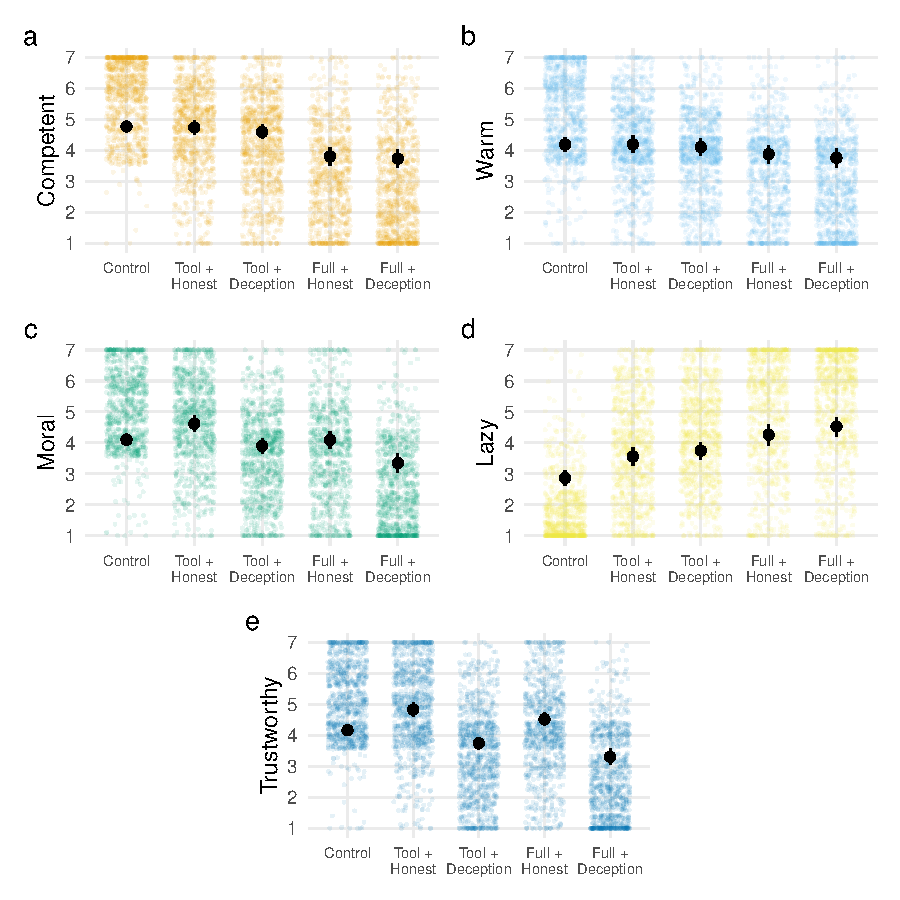
\includegraphics[keepaspectratio]{manuscript_files/figure-pdf/fig-treatments-study1-1.pdf}}
\end{center}

\noindent \emph{Note.} Participants in the control condition and four AI
outsourcing conditions evaluated people in the scenarios on (a)
competence, (b) warmth, (c) morality, (d) laziness, and (e)
trustworthiness. Coloured points represent participant responses to the
questions, jittered for easier viewing. Black points are estimated
marginal means from the fitted model, pooling over participants and
tasks. Black points and line ranges represent posterior medians and 95\%
credible intervals, respectively.

\end{figure}

\begin{table}

{\caption{{Overall Pairwise Contrasts in Study 1
\vspace{20pt}}{\label{tbl-treatment-diffs-study1}}}
\vspace{-20pt}}

\begingroup\fontsize{8}{10}\selectfont

\begin{tabular}{llllll}
\toprule
\multicolumn{1}{c}{ } & \multicolumn{5}{c}{Response} \\
\cmidrule(l{3pt}r{3pt}){2-6}
  & Competent & Warm & Moral & Lazy & Trustworthy\\
\midrule
\addlinespace[0.3em]
\multicolumn{6}{l}{\textbf{Comparison to control}}\\
\hspace{1em}Tool Honest - Control & -0.03 [-0.28 0.20] & 0.00 [-0.23 0.24] & 0.52 [0.27 0.76] & 0.70 [0.36 1.02] & 0.66 [0.44 0.90]\\
\hspace{1em}Tool Deception - Control & -0.18 [-0.41 0.06] & -0.09 [-0.32 0.15] & -0.19 [-0.44 0.05] & 0.89 [0.55 1.21] & -0.42 [-0.63 -0.21]\\
\hspace{1em}Full Honest - Control & -0.97 [-1.24 -0.70] & -0.31 [-0.56 -0.07] & 0.00 [-0.26 0.26] & 1.40 [1.02 1.76] & 0.35 [0.14 0.59]\\
\hspace{1em}Full Deception - Control & -1.04 [-1.33 -0.74] & -0.44 [-0.70 -0.16] & -0.76 [-1.04 -0.45] & 1.67 [1.30 2.04] & -0.86 [-1.12 -0.59]\\
\addlinespace[0.3em]
\multicolumn{6}{l}{\textbf{Effect of full outsourcing}}\\
\hspace{1em}Full Honest - Tool Honest & -0.93 [-1.24 -0.62] & -0.32 [-0.62 -0.01] & -0.52 [-0.86 -0.19] & 0.71 [0.28 1.13] & -0.31 [-0.59 -0.03]\\
\hspace{1em}Full Deception - Tool Deception & -0.86 [-1.21 -0.52] & -0.35 [-0.67 -0.02] & -0.56 [-0.91 -0.21] & 0.78 [0.37 1.20] & -0.44 [-0.73 -0.14]\\
\addlinespace[0.3em]
\multicolumn{6}{l}{\textbf{Effect of deception}}\\
\hspace{1em}Tool Deception - Tool Honest & -0.14 [-0.42 0.13] & -0.09 [-0.39 0.21] & -0.71 [-1.02 -0.40] & 0.19 [-0.20 0.58] & -1.09 [-1.36 -0.80]\\
\hspace{1em}Full Deception - Full Honest & -0.07 [-0.43 0.29] & -0.12 [-0.45 0.21] & -0.75 [-1.10 -0.38] & 0.26 [-0.16 0.71] & -1.21 [-1.51 -0.92]\\
\addlinespace[0.3em]
\multicolumn{6}{l}{\textbf{Interaction effect}}\\
\hspace{1em}Interaction effect & 0.08 [-0.38 0.52] & -0.04 [-0.47 0.41] & -0.04 [-0.50 0.45] & 0.07 [-0.50 0.67] & -0.12 [-0.54 0.28]\\
\bottomrule
\end{tabular}
\endgroup{}\vspace{20pt}

\vspace{-20pt}
\noindent \emph{Note.} Numbers reflect differences in marginal means on
a 7-point Likert scale, pooling over participants and tasks. The bottom
row represents the interaction between full outsourcing and deception
(i.e., the difference between the differences in the rows above). Main
numbers are posterior medians, numbers in the square brackets are 95\%
credible intervals.

\end{table}

The effects of outsourcing to AI varied across the different tasks,
especially for perceptions of warmth and morality
(Figure~\ref{fig-treatments-tasks-study1}). For example, people who used
AI for social tasks, such as writing an apology letter or a bereavement
card, were perceived as less warm, less moral, and lazier compared to
people who completed the task themselves. This was true even if the
person used AI as a tool and was honest about their usage of AI. By
contrast, we observed weaker effects of outsourcing for non-social tasks
like writing computer code or planning a syllabus.

\begin{landscape}

\begin{figure}[!htbp]

{\caption{{Variation in the Effects of Outsourcing across Tasks in Study
1 \vspace{-30pt}}{\label{fig-treatments-tasks-study1}}}}

\begin{center}
\pandocbounded{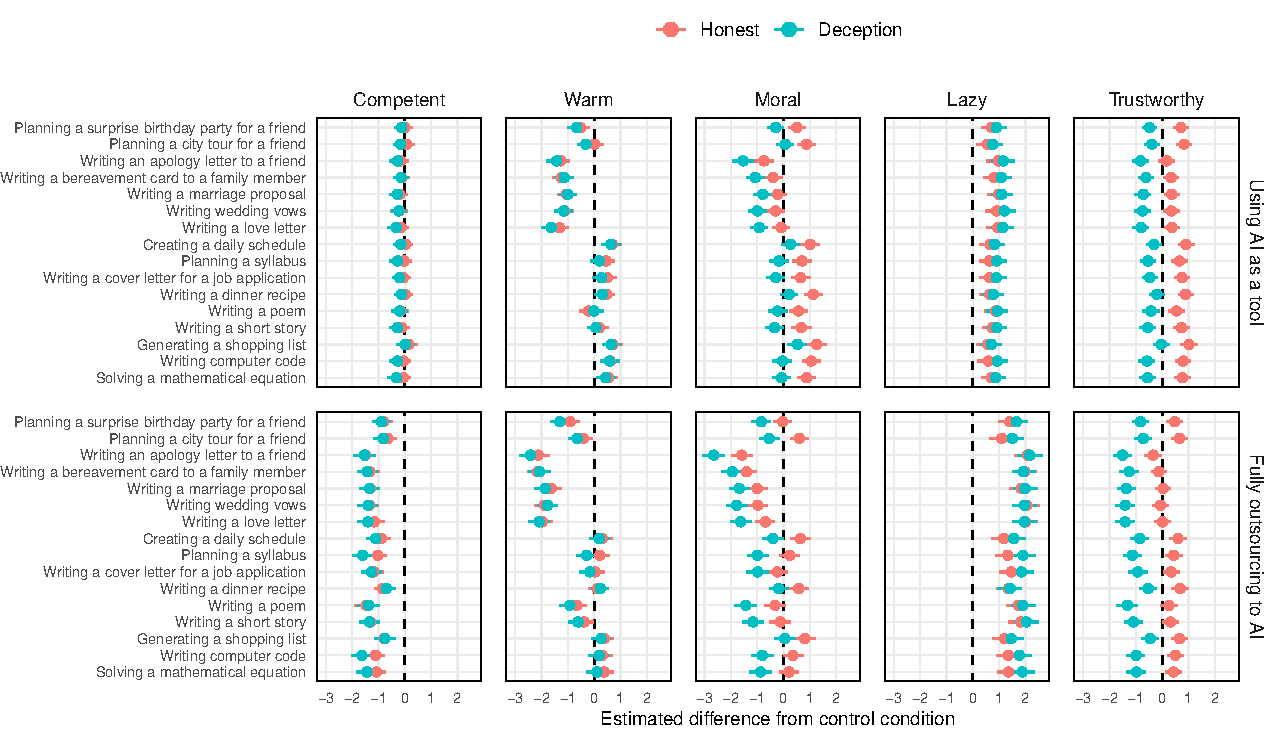
\includegraphics[keepaspectratio]{manuscript_files/figure-pdf/fig-treatments-tasks-study1-1.pdf}}
\end{center}

\vspace{-20pt}
\noindent \emph{Note.} Tasks are ordered from most social (top) to least
social (bottom) according to ratings from a pilot study. Point ranges
are differences in marginal means on a 7-point Likert scale for the
honest conditions (red) and deception conditions (blue) compared to the
control condition. Upper panels refer to the tool outsourcing
conditions, and lower panels refer to the full outsourcing conditions.
Points and ranges represent posterior medians and 95\% credible
intervals, respectively.

\end{figure}

\end{landscape}

To determine the factors that predict variation across tasks, we
incorporated ratings of tasks from a pilot study (see Supplementary
Materials for details). Participants were asked to rate the different
tasks on several features: whether the task is social, requires social
skills, impacts others, has important consequences, and requires effort.
All of these features predicted stronger causal effects of outsourcing
to AI compared to the control (Supplementary Figures
\ref{suppfig-interactions-study1} and
\ref{suppfig-interaction-pars-study1}). In other words, outsourcing to
AI is perceived more negatively for tasks that have these features,
compared to tasks without these features.

\subsection*{Discussion}\label{discussion}

In Study 1, we looked at how people who outsourced to AI in different
ways were perceived across a broad range of social and non-social tasks.
In line with our predictions, we found that ``fully'' outsourcing to AI
was perceived more negatively than using AI as a collaborative tool,
particularly for socio-relational tasks. We also found, predictably,
that people were seen as less moral and less trustworthy if they did not
acknowledge their use of AI. Importantly, though, we show that even
using AI in the ``best'' way -- only as a tool and being honest about
one's usage -- still led to negative social perceptions for the more
socio-relational tasks like writing a love letter, an apology, or
wedding vows.

In Study 2, we investigate whether these negative perceptions extend to
the work itself and remain after seeing the output. It could be, for
example, that someone is perceived badly for using ChatGPT to write
their bereavement card, but the writing itself is seen as equally
well-written and authentic, if not more so, than if the person had
written the card themselves. Indeed, evidence suggests that text
generated by ChatGPT is rated as higher quality than human-written text
(\citeproc{ref-Noy2023}{Noy \& Zhang, 2023}). Moreover, it is possible
that seeing appropriate output could mitigate negative perceptions by
highlighting how the AI can in fact perform the task well. We explored
these possibilities in Study 2.

\section*{Study 2}\label{study-2}

\subsection*{Methods}\label{methods-1}

\subsubsection*{Participants}\label{participants-1}

We conducted a power simulation to determine our target sample size. The
simulation suggested that a sample size of 125 participants per
condition (overall \emph{n} = 750 for six conditions) would be required
to detect a small-to-medium difference between conditions (Cohen's
\emph{d} ≈ 0.40) with above 80\% power.

We recruited a convenience sample of 800 participants from the United
Kingdom through Prolific. After excluding participants who failed our
pre-treatment attention check, we were left with a final sample of 766
participants (425 female; 337 male; 3 non-binary / third gender; 1
undisclosed gender; mean age = 41.93 years). 72\% of these participants
reported having used ChatGPT before.

\subsubsection*{Design}\label{design-1}

We randomly allocated participants to one of six conditions in a 3x2
between-subjects design. We manipulated the type of outsourcing:
(\emph{i}) no outsourcing control, (\emph{ii}) using AI as a tool, and
(\emph{iii}) fully outsourcing to AI. Here, in contrast to Study 1, we
also explicitly manipulated whether the task prompt was social or
non-social.

\subsubsection*{Procedure}\label{procedure-1}

We told participants that they would read and evaluate a short piece of
writing from ``another participant''. In reality, we generated the
writing using ChatGPT version 4o. We asked ChatGPT to generate a 300
word response to the prompt and to write convincingly like a real human.
We then edited the text to appear more human-like by, for example,
removing classic AI markers like dashes and concluding sentences and
ensuring that the information was not too generic, such that the writing
could reasonably be attributed to both a human and AI.

The prompt for the piece of writing varied between conditions:

\begin{itemize}
\tightlist
\item
  \emph{Social conditions}: ``Please write a description of a close
  family member or friend, explaining why they are special to you.''
\item
  \emph{Non-social conditions}: ``Please write a short description of a
  book, TV show, or film of your choice.''
\end{itemize}

We explained that the ``other participant'' was asked several questions
about how they produced their answer, including whether or not they used
an AI tool like ChatGPT. We explained that the participant was
encouraged to be honest and told that they would be paid regardless. The
response from the ``other participant'' varied between conditions:

\begin{itemize}
\tightlist
\item
  \emph{Control conditions}: ``The participant reported that they did
  not use any AI tool like ChatGPT. Instead, they worked on the response
  themselves from start to finish.''
\item
  \emph{Tool outsourcing conditions}: ``The participant reported using
  ChatGPT to provide ideas, inspiration, and feedback. The participant
  told us that they edited and rewrote ChatGPT's suggestions and
  finished writing the response themselves.''
\item
  \emph{Full outsourcing conditions}: ``The participant reported using
  ChatGPT to complete the task. The participant told us that they copied
  ChatGPT's output word-for-word, rather than producing the response
  themselves.''
\end{itemize}

Next, we presented participants with a randomly-chosen pre-generated
essay answer to the prompt (see Supplementary Tables
\ref{supptbl-essay-answers-social-study2} and
\ref{supptbl-essay-answers-nonsocial-study2} for full essay answers). In
the social conditions, the answer either referred to the participant's
father, their sister, or their best friend. In the non-social
conditions, the answer either referred to the book The Hobbit, the TV
show Buffy the Vampire Slayer, or the film Titanic. Reading times and
responses to a follow-up comprehension question suggested that
participants read the essay answers in sufficient detail (see
Supplementary Table~\ref{supptbl-essay-comprehension-study2}).

Finally, we asked participants about their perceptions of the essay
answer and the ``other participant''. We asked how well-written,
meaningful, and authentic they thought the answer was (7-point Likert
scales), what letter grade they would give the answer (A-E), and how
much they would hypothetically reward the other participant for their
work (from £0.00 to £1.00). We also asked how well each of the following
words described the other participant: competent, warm, moral, lazy, and
trustworthy (7-point Likert scales).

At the end of the study, we gave participants a manipulation check and
asked them whether they believed the manipulation. Almost all
participants correctly reported the condition that they were in and most
participants stated that they believed the essay response was written in
the way we described, suggesting that the manipulation was successful
(see Supplementary Table~\ref{supptbl-manipulation-check-study2}). We
also asked participants several questions about ChatGPT.

\subsubsection*{Pre-registration}\label{pre-registration-1}

We pre-registered the study on the Open Science Framework\footnote{Due
  to a technical error with archiving this pre-registration on the Open
  Science Framework, the timestamp for the registration was lost.
  However, on our OSF project
  (\url{https://osf.io/xhmzk/?view_only=a4da193574d7410ba4d2aa3945a28b05}),
  it is possible to view our pre-registration document file and its
  timestamped upload date.}.

\subsubsection*{Statistical Analysis}\label{statistical-analysis-1}

We fitted two Bayesian multilevel models to the data. The first model
was a multivariate cumulative-link ordinal model including all Likert
scales as separate response variables. The second model was a
zero-one-inflated-beta model applied specifically to the reward
question, which was a slider scale varying between 0 and 1. For both
models, we included fixed effects for the interaction between
outsourcing type and task type and varying intercepts and slopes for
essay answers. We used regularising priors for all parameters to impose
conservatism on parameter estimates. All models converged normally
(\(\hat{R}\) ≤ 1.01).

\subsection*{Results}\label{results-1}

We first looked at character evaluations. We found that even when
provided with concrete output, people were still perceived more
negatively across all character evaluations if they outsourced the
writing task to AI, either by using ChatGPT as a collaborative tool or
by copying the text from ChatGPT verbatim
(Supplementary Figure~\ref{suppfig-treatments-person-study2};
Supplementary Table~\ref{supptbl-treatment-diffs-person-study2}). In
contrast to Study 1, however, we did not find any differences in
character evaluations between the tool outsourcing and full outsourcing
conditions. We did not find differences in character evaluations between
social and non-social tasks and did not find any interaction effects.

Turning to evaluations of the work itself, we found that the
AI-outsourced work (either outsourced by using AI as a collaborative
tool or fully outsourced) was judged as being equally well written to
the work in the control condition
(Figure~\ref{fig-treatments-work-study2};
Table~\ref{tbl-treatment-diffs-work-study2}). This is in line with the
writing indeed being identical in all conditions. Interestingly,
however, we found that essay responses that were ostensibly generated
using AI were perceived as less meaningful and less authentic compared
to essay responses ostensibly written by a human. Participants also
marked AI-generated essays with a lower grade and rewarded AI-generated
essays with a lower hypothetical monetary bonus. In contrast to Study 1,
we did not find differences in perceptions of the work between the tool
outsourcing and full outsourcing conditions, except for the reward
question, where fully outsourced essays (i.e., essays copied verbatim
from ChatGPT) were rewarded £0.23 less than essays generated using AI as
a collaborative tool. We did not find any differences between social and
non-social tasks and did not find any interaction effects.

\begin{figure}[!htbp]

{\caption{{Perceptions of the Work in Study
2}{\label{fig-treatments-work-study2}}}}

\begin{center}
\pandocbounded{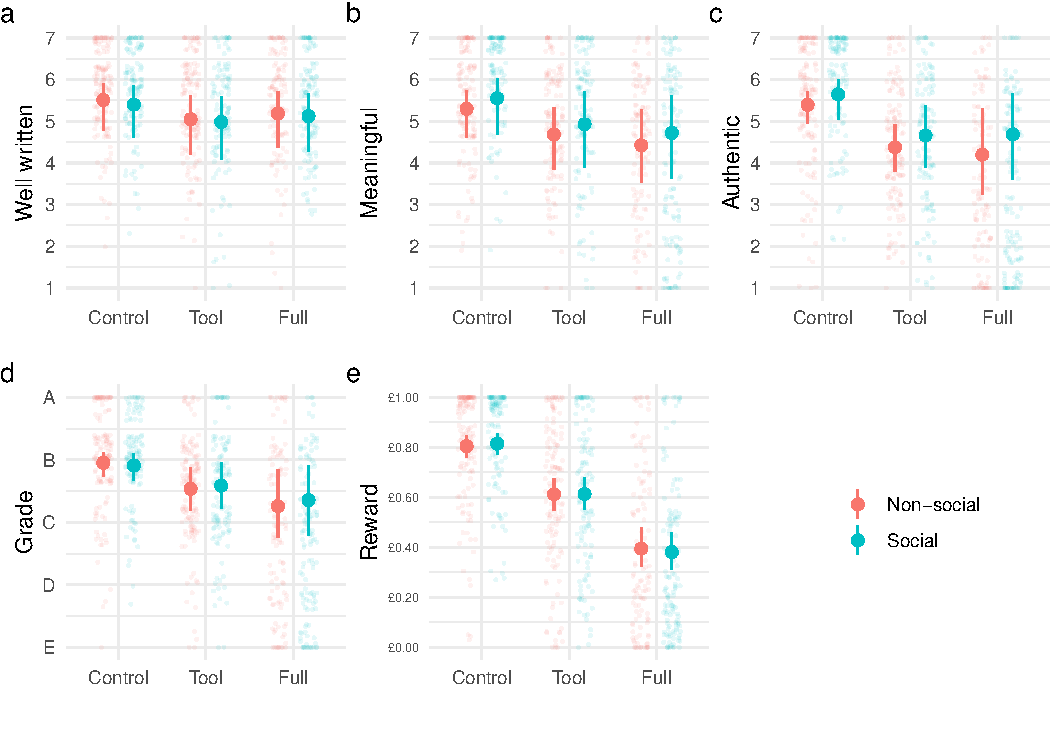
\includegraphics[keepaspectratio]{manuscript_files/figure-pdf/fig-treatments-work-study2-1.pdf}}
\end{center}

\vspace{-20pt}
\noindent \emph{Note.} Participants in the control condition, the tool
outsourcing condition, and the full outsourcing condition evaluated the
essay response to the writing task. Participants rated whether the essay
response was (a) well-written, (b) meaningful, and (c) authentic.
Participants also (d) graded the work and (e) rewarded the work with a
hypothetical monetary bonus. Jittered points represent participant
responses to the questions, split by whether the writing task was a
non-social task (red) or a social task (blue). Point ranges are
estimated marginal means from the fitted model, pooling over essay
answers. Points and line ranges represent posterior medians and 95\%
credible intervals, respectively.

\end{figure}

\begin{table}

{\caption{{Pairwise Contrasts for Perceptions of the Work in Study 2
\vspace{20pt}}{\label{tbl-treatment-diffs-work-study2}}}
\vspace{-20pt}}

\begingroup\fontsize{7.5}{9.5}\selectfont

\begin{tabular}{llllll}
\toprule
\multicolumn{1}{c}{ } & \multicolumn{5}{c}{Response} \\
\cmidrule(l{3pt}r{3pt}){2-6}
  & Well written & Meaningful & Authentic & Grade & Reward\\
\midrule
\addlinespace[0.3em]
\multicolumn{6}{l}{\textbf{Effect of outsourcing type}}\\
\addlinespace[0.3em]
\multicolumn{6}{l}{\textbf{  Task type = Social}}\\
\hspace{1em}Tool Social - Control Social & -0.42 [-0.84 0.03] & -0.64 [-1.11 -0.08] & -1.01 [-1.47 -0.35] & -0.33 [-0.60 -0.02] & -0.20 [-0.27 -0.13]\\
\hspace{1em}Full Social - Control Social & -0.28 [-0.63 0.09] & -0.84 [-1.55 -0.06] & -0.95 [-1.93 -0.07] & -0.55 [-1.07 -0.04] & -0.43 [-0.50 -0.36]\\
\hspace{1em}Full Social - Tool Social & 0.14 [-0.39 0.67] & -0.21 [-1.13 0.74] & 0.04 [-1.12 1.12] & -0.23 [-0.84 0.36] & -0.23 [-0.32 -0.14]\\
\addlinespace[0.3em]
\multicolumn{6}{l}{\textbf{  Task type = Non-social}}\\
\hspace{1em}Tool Non-social - Control Non-social & -0.46 [-0.92 -0.02] & -0.62 [-1.09 -0.08] & -1.03 [-1.47 -0.49] & -0.42 [-0.71 -0.07] & -0.19 [-0.26 -0.12]\\
\hspace{1em}Full Non-social - Control Non-social & -0.32 [-0.70 0.03] & -0.90 [-1.56 -0.08] & -1.23 [-2.09 -0.12] & -0.71 [-1.16 -0.13] & -0.41 [-0.49 -0.32]\\
\hspace{1em}Full Non-social - Tool Non-social & 0.14 [-0.39 0.71] & -0.28 [-1.06 0.62] & -0.21 [-1.19 0.97] & -0.29 [-0.86 0.34] & -0.22 [-0.31 -0.12]\\
\addlinespace[0.3em]
\multicolumn{6}{l}{\textbf{Effect of task type}}\\
\hspace{1em}Control Social - Control Non-social & -0.10 [-0.56 0.33] & 0.28 [-0.36 0.73] & 0.27 [-0.21 0.64] & -0.04 [-0.27 0.17] & 0.01 [-0.05 0.06]\\
\hspace{1em}Tool Social - Tool Non-social & -0.06 [-0.67 0.56] & 0.27 [-0.61 0.99] & 0.29 [-0.41 0.95] & 0.04 [-0.30 0.41] & 0.00 [-0.09 0.09]\\
\hspace{1em}Full Social - Full Non-social & -0.07 [-0.64 0.51] & 0.30 [-0.59 1.15] & 0.48 [-0.37 1.38] & 0.09 [-0.33 0.57] & -0.02 [-0.12 0.09]\\
\addlinespace[0.3em]
\multicolumn{6}{l}{\textbf{Interaction effect}}\\
\hspace{1em}Interaction: Tool - Control & 0.05 [-0.39 0.51] & -0.02 [-0.52 0.56] & 0.02 [-0.51 0.62] & 0.09 [-0.22 0.39] & -0.01 [-0.10 0.08]\\
\hspace{1em}Interaction: Full - Control & 0.04 [-0.34 0.46] & 0.03 [-0.59 0.73] & 0.23 [-0.50 1.02] & 0.13 [-0.23 0.55] & -0.03 [-0.12 0.08]\\
\hspace{1em}Interaction: Full - Tool & 0.00 [-0.58 0.55] & 0.05 [-0.74 0.89] & 0.21 [-0.66 1.12] & 0.05 [-0.43 0.53] & -0.01 [-0.13 0.10]\\
\bottomrule
\end{tabular}
\endgroup{}\vspace{20pt}

\vspace{-20pt}
\noindent \emph{Note.} Numbers reflect differences in marginal means on
either a 7-point Likert scale (well-written, meaningful, authentic), a
5-point ordinal grade scale (grade), or a 0-1 sliding scale (reward).
Estimates are pooled over essay answers. The bottom rows represent the
interactions between outsourcing type and task type. Main numbers are
posterior medians, numbers in the square brackets are 95\% credible
intervals.

\end{table}

\subsection*{Discussion}\label{discussion-1}

In Study 2, we turned to look at how people perceived both the
outsourcer and the outsourced work when given specific output in a
social or non-social task that was described as being produced
independently by a person, produced by a person in collaboration with AI
as a tool, or outsourced in full to AI. We find that our results
generalise from character judgments to perceptions of the work itself:
text purportedly generated using AI was perceived to be less meaningful,
less authentic, and less reward-worthy compared to the same text
described as human-generated.

Surprisingly, we found no differences in the effect of AI-outsourcing
between social and non-social tasks. This may be due to the particular
tasks we chose. Writing \emph{about} someone close to you is not quite
the same as writing something \emph{for} someone close to you, as is the
case with wedding vows, love letters, and bereavement cards. We also
found no differences between the tool and full outsourcing conditions,
aside from the lower rewards given to participants in the latter
condition. It is possible that because the set-up described to
participants was of another participant who was asked to produce work on
Prolific and then admitted they used AI, participants saw any kind of AI
use as violating an implicit contract between the survey requester and
respondent and judged them negatively accordingly.

In Study 3, we turn to explore potential mechanisms driving our effects.
We assume that effort may play a role, since perceived effort is often
used as a signal of one's moral character
(\citeproc{ref-Cubitt2011}{Cubitt et al., 2011}) and cooperative intent
(\citeproc{ref-Celniker2023}{Celniker et al., 2023}). Study 2 also
suggested a role of authenticity: in line with work on the psychological
importance of authenticity (\citeproc{ref-Newman2019}{Newman, 2019}),
people who outsource to AI may be perceived as producing work that is
less authentically their own, leading to negative evaluations. To
explore these potential mechanisms, we experimentally manipulate (1) how
much effort someone puts into the task and (2) whether they outsource
the task to a standard LLM like ChatGPT or a personalised LLM trained
specifically on their own prior writings (and so therefore producing
work that is more authentically ``theirs''). We expected negative
perceptions of outsourcing to be mitigated when the person uses a
personalised LLM and expends significant effort on formulating prompts
for the AI.

\section*{Study 3}\label{study-3}

\subsection*{Methods}\label{methods-2}

\subsubsection*{Participants}\label{participants-2}

We used the same power estimate from Study 1 to determine our target
sample size of \emph{n} = 750 (150 participants in each of five
conditions). We recruited a convenience sample of 802 participants from
the United Kingdom through Prolific. After excluding participants who
failed our pre-treatment attention check, we were left with a final
sample of 753 participants (462 female; 278 male; 9 non-binary / third
gender; 4 undisclosed gender; mean age = 44.29 years). 74\% of these
participants reported having used ChatGPT before.

\subsubsection*{Design}\label{design-2}

We used the same ``control plus 2x2'' between-subjects design as in
Study 1. In the experimental conditions, we manipulated whether people
in the scenarios used a standard or personalised AI model, and whether
people put more or less effort into the task. This resulted in five
conditions overall: (\emph{i}) the control condition, (\emph{ii}) the
standard-low-effort condition, (\emph{iii}) the standard-high-effort
condition, (\emph{iv}) the personalised-low-effort condition, and
(\emph{v}) the personalised-high-effort condition. Our authenticity
manipulation was inspired by recent psychological work looking at the
credit-blame asymmetry in AI use (\citeproc{ref-Earp2024}{Earp et al.,
2024}), showing that people receive more personal credit for their work
when they use an AI model trained on their own prior writings.

\subsubsection*{Procedure}\label{procedure-2}

The procedure was mostly identical to Study 1 to allow us to explore
effects across a range of tasks, but we updated the study preamble and
the presentation of the scenarios. For participants in the personalised
AI conditions, we expanded the study preamble to explain that
personalised AI models were trained on people's own prior writings and
``tailored to each specific person and their own thoughts, feelings, and
values''. Then in the scenarios, we told participants in the
experimental conditions:

\begin{itemize}
\tightlist
\item
  \emph{Standard AI conditions}: ``In order to complete this task,
  {[}the person{]} uses the AI tool ChatGPT.''
\item
  \emph{Personalised AI conditions}: ``In order to complete this task,
  {[}the person{]} uses a personalised AI tool.''
\end{itemize}

We then told participants:

\begin{itemize}
\tightlist
\item
  \emph{Low effort conditions}: ``{[}The person{]} quickly gives the AI
  a rushed prompt and uses its first output.''
\item
  \emph{High effort conditions}: ``{[}The person{]} carefully gives the
  AI several detailed prompts and, after multiple rounds of changes,
  uses its resulting output.''
\end{itemize}

At the end of the study, we asked participants to choose which of these
was more authentic and effortful, respectively. 94\% of participants
stated that the personalised AI was more authentic and 99\% of
participants stated that giving the AI several detailed prompts was more
effortful. This suggests that even if participants might not have felt
the output was meaningfully authentic in the way that mattered (see
Discussion), our participants agreed that using a personalised AI was at
least more authentic than using a generic one.

\subsubsection*{Pre-registration}\label{pre-registration-2}

We pre-registered the study on the Open Science Framework
(\url{https://osf.io/ac9g3/?view_only=912d9b57023d49baa87eea999574f0ce}).

\subsubsection*{Statistical Analysis}\label{statistical-analysis-2}

We fitted the same Bayesian multivariate multilevel cumulative-link
ordinal models as in Studies 1 and 2. All models converged normally
(\(\hat{R}\) ≤ 1.01).

\subsection*{Results}\label{results-2}

We first looked across all the tasks. On average, we found that people
who outsourced to AI in a low effort way were perceived as less
competent, less moral, lazier, and less trustworthy than people who put
more effort into their use of AI (Figure~\ref{fig-treatments-study3};
Table~\ref{tbl-treatment-diffs-study3}). By contrast, we found that
character evaluations did not differ between people who used a standard
AI model rather than a personalised AI model. We also found no
interaction effects between effort and the type of AI used.

\begin{figure}[!htbp]

{\caption{{Overall Character Evaluations in Study
3}{\label{fig-treatments-study3}}}}

\begin{center}
\pandocbounded{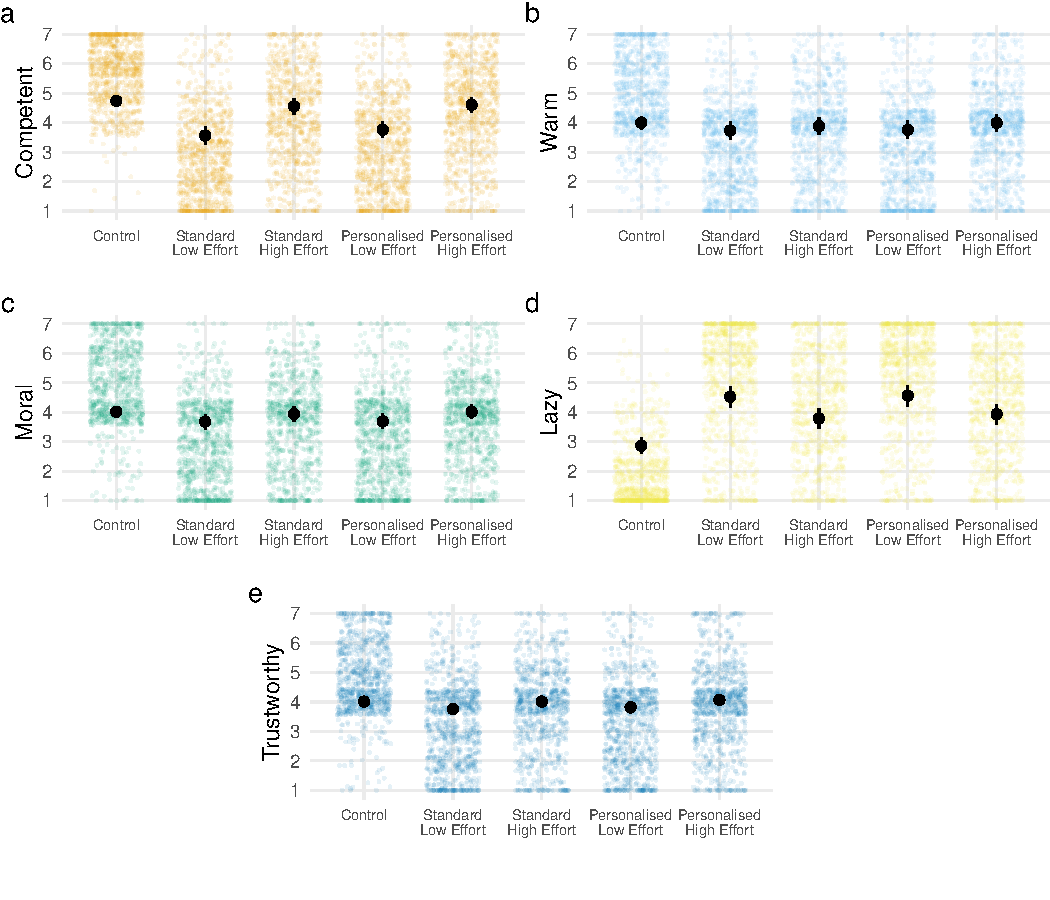
\includegraphics[keepaspectratio]{manuscript_files/figure-pdf/fig-treatments-study3-1.pdf}}
\end{center}

\vspace{-20pt}
\noindent \emph{Note.} Participants in the control condition and four AI
outsourcing conditions evaluated people in the scenarios on (a)
competence, (b) warmth, (c) morality, (d) laziness, and (e)
trustworthiness. Coloured points represent participant responses to the
questions, jittered for easier viewing. Black points are estimated
marginal means from the fitted model, pooling over participants and
tasks. Black points and line ranges represent posterior medians and 95\%
credible intervals, respectively.

\end{figure}

\begin{table}

{\caption{{Overall Pairwise Contrasts in Study 3
\vspace{20pt}}{\label{tbl-treatment-diffs-study3}}}
\vspace{-20pt}}

\begingroup\fontsize{7}{9}\selectfont

\begin{tabular}{llllll}
\toprule
\multicolumn{1}{c}{ } & \multicolumn{5}{c}{Response} \\
\cmidrule(l{3pt}r{3pt}){2-6}
  & Competent & Warm & Moral & Lazy & Trustworthy\\
\midrule
\addlinespace[0.3em]
\multicolumn{6}{l}{\textbf{Comparison to control}}\\
\hspace{1em}Standard Low Effort - Control & -1.18 [-1.49 -0.84] & -0.26 [-0.52 0.00] & -0.34 [-0.59 -0.10] & 1.67 [1.24 2.06] & -0.26 [-0.45 -0.06]\\
\hspace{1em}Standard High Effort - Control & -0.19 [-0.45 0.08] & -0.11 [-0.36 0.13] & -0.08 [-0.31 0.15] & 0.93 [0.54 1.31] & 0.00 [-0.18 0.18]\\
\hspace{1em}Personalised Low Effort - Control & -0.98 [-1.25 -0.71] & -0.24 [-0.51 0.02] & -0.33 [-0.57 -0.08] & 1.70 [1.28 2.09] & -0.19 [-0.38 -0.01]\\
\hspace{1em}Personalised High Effort - Control & -0.13 [-0.38 0.14] & 0.00 [-0.24 0.23] & 0.00 [-0.23 0.22] & 1.08 [0.68 1.44] & 0.05 [-0.12 0.23]\\
\addlinespace[0.3em]
\multicolumn{6}{l}{\textbf{Effect of AI type}}\\
\hspace{1em}Standard Low Effort - Personalised Low Effort & -0.20 [-0.54 0.17] & -0.03 [-0.36 0.30] & -0.01 [-0.32 0.30] & -0.04 [-0.51 0.44] & -0.06 [-0.29 0.17]\\
\hspace{1em}Standard High Effort - Personalised High Effort & -0.05 [-0.38 0.27] & -0.11 [-0.41 0.20] & -0.08 [-0.37 0.22] & -0.15 [-0.62 0.33] & -0.05 [-0.28 0.18]\\
\addlinespace[0.3em]
\multicolumn{6}{l}{\textbf{Effect of effort}}\\
\hspace{1em}Standard Low Effort - Standard High Effort & -1.00 [-1.35 -0.61] & -0.15 [-0.46 0.17] & -0.26 [-0.56 0.04] & 0.74 [0.26 1.21] & -0.25 [-0.50 -0.01]\\
\hspace{1em}Personalised Low Effort - Personalised High Effort & -0.85 [-1.17 -0.53] & -0.24 [-0.55 0.10] & -0.32 [-0.63 -0.02] & 0.63 [0.14 1.08] & -0.25 [-0.48 -0.02]\\
\addlinespace[0.3em]
\multicolumn{6}{l}{\textbf{Interaction effect}}\\
\hspace{1em}Interaction effect & -0.15 [-0.62 0.35] & 0.09 [-0.36 0.52] & 0.06 [-0.36 0.49] & 0.10 [-0.55 0.77] & 0.00 [-0.35 0.32]\\
\bottomrule
\end{tabular}
\endgroup{}\vspace{20pt}

\vspace{-20pt}
\noindent \emph{Note.} Numbers reflect differences in marginal means on
a 7-point Likert scale, pooling over participants and tasks. The bottom
row represents the interaction between AI type and effort (i.e., the
difference between the differences in the rows above). Main numbers are
posterior medians, numbers in the square brackets are 95\% credible
intervals.

\end{table}

As in Study 1, the effects of outsourcing to AI varied across the
different tasks, especially for perceptions of warmth and morality
(Figure~\ref{fig-treatments-tasks-study3}). We again found that the
negative causal effects of outsourcing to AI were particularly strong
for tasks that are social, require social skills, impact others, have
important consequences, and require effort (Supplementary Figures
\ref{suppfig-interactions-study3} and
\ref{suppfig-interaction-pars-study3}). Indeed, for tasks like writing
wedding vows or writing a love letter, outsourcing to a personalised AI
in a high effort way was still perceived more negatively than the
control condition for all five character dimensions.

\begin{landscape}

\begin{figure}[!htbp]

{\caption{{Variation in the Effects of Outsourcing across Tasks in Study
3 \vspace{-30pt}}{\label{fig-treatments-tasks-study3}}}}

\begin{center}
\pandocbounded{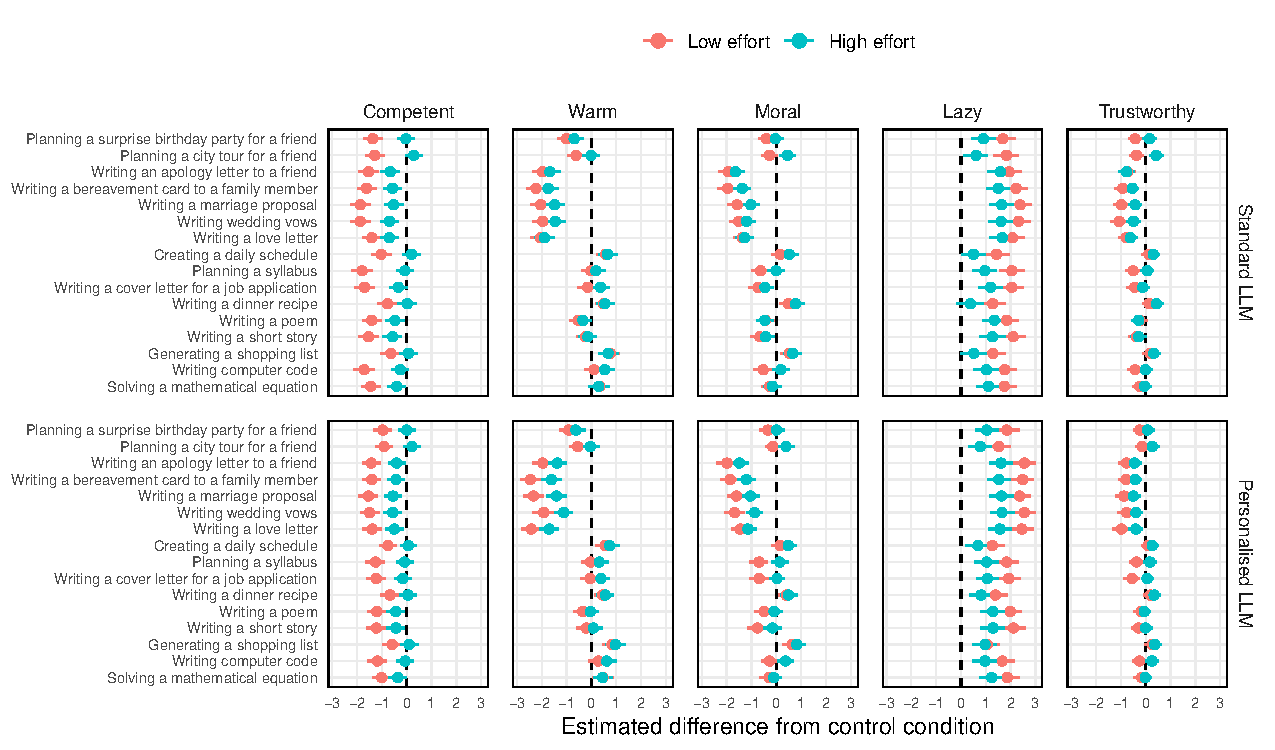
\includegraphics[keepaspectratio]{manuscript_files/figure-pdf/fig-treatments-tasks-study3-1.pdf}}
\end{center}

\vspace{-20pt}
\noindent \emph{Note.} Tasks are ordered from most social (top) to least
social (bottom) according to ratings from a pilot study. Point ranges
are differences in marginal means on a 7-point Likert scale for the low
effort conditions (red) and high effort conditions (blue) compared to
the control condition. Upper panels refer to the standard LLM
conditions, and lower panels refer to the personalised LLM conditions.
Points and ranges represent posterior medians and 95\% credible
intervals, respectively.

\end{figure}

\end{landscape}

\subsection*{Discussion}\label{discussion-2}

In Study 3, we found that effort is an important mechanism by which
outsourcing to AI leads to negative character evaluations. People who
engaged in effortless copying of the AI's first output were perceived
more negatively than people who spent time and effort crafting the AI's
output with multiple prompts. Nevertheless, for social tasks like
writing wedding vows or love letters, outsourcing to AI in a high effort
way was still perceived more negatively than completing the task
oneself.

Interestingly, we found no effect of authenticity as proxied by the use
of a personalised AI that is trained on one's own prior writings
compared to a standard AI like ChatGPT. This could indicate that
authenticity is not an important mechanism underlying the effect of
outsourcing on negative character evaluations. However, our specific
manipulation may not have moved the needle on authenticity enough to
impact character evaluations. While previous work has found an effect of
personalised AI models on perceived credit (\citeproc{ref-Earp2024}{Earp
et al., 2024}), and the majority of participants in our study stated
that the personalised AI was more authentic than a standard model like
ChatGPT, it is possible that perceptions of \emph{meaningful}
authenticity in our study remained low even with the personalised AI
model. An AI could be perfectly trained on all apologies that a person
has ever written, but one might still think that a specific apology it
then generates in a new instance is not an \emph{authentic} apology.
Therefore, even if people were described as outsourcing to an AI that
was trained on their own writing and therefore personalised,
participants still may not have seen the specific output as being
meaningfully authentic in the way that matters for character judgments.

In Study 4, we turn to look at a third potential mechanism: a perceived
lack of importance attached to the task. When participants read about
someone who outsources to AI in our studies, they may be inferring that
they simply did not care enough about the task -- ``If this was
important to them, they would do it themselves!''. To the extent that we
especially want people to care about their relationships with others --
the kind of things demonstrated through love letters, apology notes, and
gift-giving -- this could explain the particular negativity we see for
social tasks compared to tasks like writing daily schedules, recipes, or
computer code. To test this, in Study 4, we attempted to counteract
inferences about care for the task by explicitly telling participants
that someone had a good reason for using AI: that they really cared
about the task and used AI because they wanted to get it right.

\section*{Study 4}\label{study-4}

\subsection*{Methods}\label{methods-3}

\subsubsection*{Participants}\label{participants-3}

We used the same power estimate from Study 1 to determine our target
sample size of \emph{n} = 750 (150 participants in each of five
conditions). We recruited a convenience sample of 800 participants from
the United Kingdom through Prolific. After excluding participants who
failed our pre-treatment attention check, we were left with a final
sample of 758 participants (398 female; 346 male; 8 non-binary / third
gender; 6 undisclosed gender; mean age = 41.72 years). 80\% of these
participants reported having used ChatGPT before.

\subsubsection*{Design}\label{design-3}

We used the same ``control plus 2x2'' between-subjects design as in
Studies 1 and 3. In the experimental conditions, we manipulated whether
people in the scenarios used AI as a tool or ``fully'' outsourced to AI,
and whether people had bad or good reasons for using AI. This resulted
in five conditions overall: (\emph{i}) the control condition,
(\emph{ii}) the tool-bad-reason condition, (\emph{iii}) the
tool-good-reason condition, (\emph{iv}) the full-bad-reason condition,
and (\emph{v}) the full-good-reason condition.

\subsubsection*{Procedure}\label{procedure-3}

The procedure was mostly identical to Study 3, with two changes. First,
we reduced the number of tasks, focusing on eight tasks (four ``social''
tasks and four ``non-social'' tasks) that fit with the manipulation of
the updated design (since, for example, participants might find it
difficult to see how someone could deeply value a shopping list and want
to get it right). Second, we updated the presentation of the scenarios.
We told participants in the experimental conditions:

\begin{itemize}
\tightlist
\item
  \emph{Bad reason conditions}: ``Because they are really short on time
  and want to complete the task quickly, {[}the person{]} uses the AI
  tool ChatGPT.''
\item
  \emph{Good reason conditions}: ``Because this task is really important
  to them and they want to make sure they get it right, {[}the person{]}
  uses the AI tool ChatGPT.''
\end{itemize}

We then told participants:

\begin{itemize}
\tightlist
\item
  \emph{Tool outsourcing conditions}: ``{[}The person{]} asks ChatGPT to
  provide ideas, inspiration, and feedback, but they edit and rewrite
  the suggestions and finish the task themselves.''
\item
  \emph{Full outsourcing conditions}: ``{[}The person{]} copies
  ChatGPT's output word-for-word, rather than doing it themselves.''
\end{itemize}

In addition to the five character evaluations, on each page we also
asked participants, on a 7-point Likert scale, how much they thought the
person cared about the task.

\subsubsection*{Pre-registration}\label{pre-registration-3}

We pre-registered the study on the Open Science Framework
(\url{https://osf.io/ac9g3/?view_only=912d9b57023d49baa87eea999574f0ce}).

\subsubsection*{Statistical Analysis}\label{statistical-analysis-3}

We fitted the same Bayesian multivariate multilevel cumulative-link
ordinal models as in Studies 1 and 3. All models converged normally
(\(\hat{R}\) ≤ 1.01).

\subsection*{Results}\label{results-3}

We first looked across all the tasks. In line with our previous results,
we found that people who fully outsourced to AI by copying the output
verbatim were perceived as less competent, less moral, and less
trustworthy than people who used AI as a collaborative tool
(Figure~\ref{fig-treatments-study4};
Table~\ref{tbl-treatment-diffs-study4}). Perhaps surprisingly, though,
people's reasons for outsourcing to AI did not appear to influence
character evaluations when pooling across all the tasks. When looking at
the tasks overall, character evaluations did not differ between people
who really cared about the task and wanted to get it right and people
who used AI because they were short on time and wanted to complete the
task quickly. This was true both when using the AI as a tool or
outsourcing in full.

\begin{figure}[!htbp]

{\caption{{Overall Character Evaluations in Study
4}{\label{fig-treatments-study4}}}}

\begin{center}
\pandocbounded{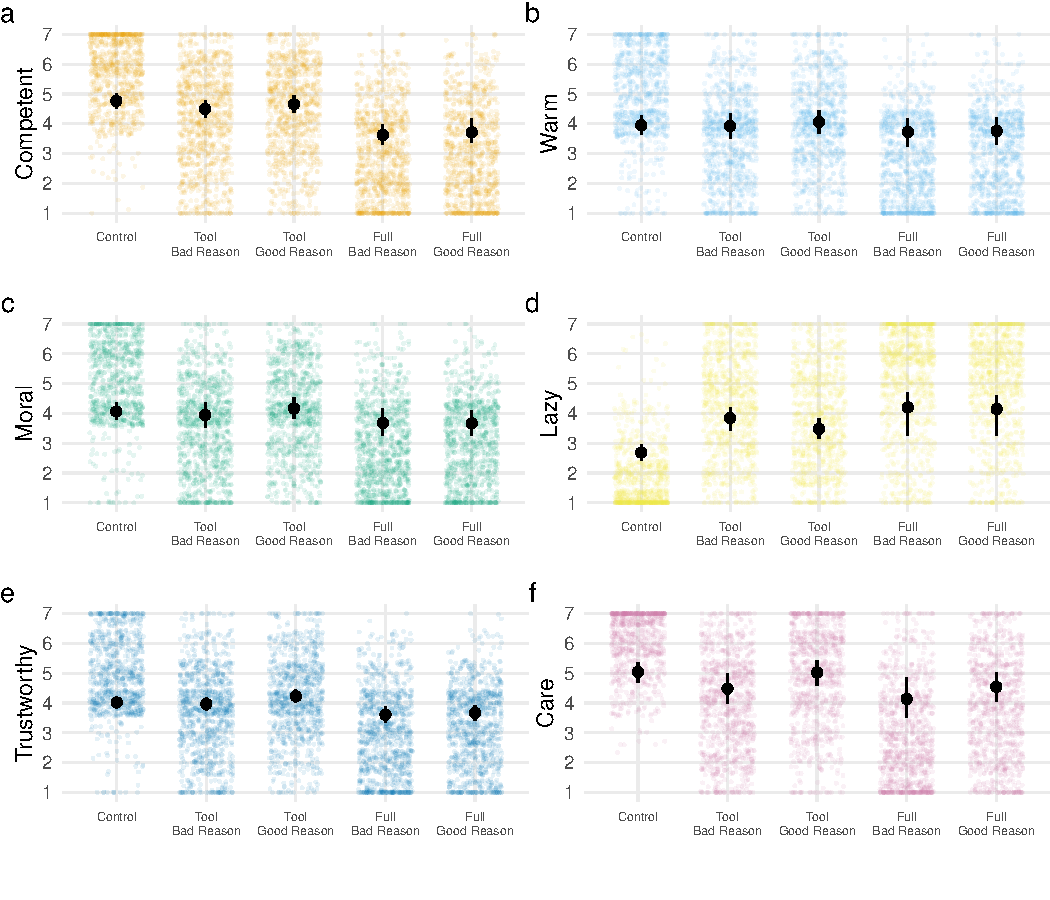
\includegraphics[keepaspectratio]{manuscript_files/figure-pdf/fig-treatments-study4-1.pdf}}
\end{center}

\vspace{-20pt}
\noindent \emph{Note.} Participants in the control condition and four AI
outsourcing conditions evaluated people in the scenarios on (a)
competence, (b) warmth, (c) morality, (d) laziness, and (e)
trustworthiness. Coloured points represent participant responses to the
questions, jittered for easier viewing. Black points are estimated
marginal means from the fitted model, pooling over participants and
tasks. Black points and line ranges represent posterior medians and 95\%
credible intervals, respectively.

\end{figure}

\begin{landscape}

\begin{table}

{\caption{{Overall Pairwise Contrasts in Study 4
\vspace{20pt}}{\label{tbl-treatment-diffs-study4}}}
\vspace{-20pt}}

\begingroup\fontsize{8.5}{10.5}\selectfont

\begin{tabular}{lllllll}
\toprule
\multicolumn{1}{c}{ } & \multicolumn{6}{c}{Response} \\
\cmidrule(l{3pt}r{3pt}){2-7}
  & Competent & Warm & Moral & Lazy & Trustworthy & Care\\
\midrule
\addlinespace[0.3em]
\multicolumn{7}{l}{\textbf{Comparison to control}}\\
\hspace{1em}Tool Bad Reason - Control & -0.27 [-0.53 -0.02] & -0.03 [-0.36 0.30] & -0.12 [-0.46 0.23] & 1.16 [0.73 1.54] & -0.05 [-0.27 0.17] & -0.56 [-0.97 -0.11]\\
\hspace{1em}Tool Good Reason - Control & -0.11 [-0.38 0.13] & 0.11 [-0.20 0.42] & 0.10 [-0.19 0.39] & 0.80 [0.40 1.17] & 0.21 [-0.01 0.43] & -0.02 [-0.38 0.34]\\
\hspace{1em}Full Bad Reason - Control & -1.15 [-1.42 -0.82] & -0.22 [-0.60 0.15] & -0.39 [-0.76 0.02] & 1.57 [0.70 2.01] & -0.41 [-0.68 -0.13] & -0.92 [-1.46 -0.28]\\
\hspace{1em}Full Good Reason - Control & -1.07 [-1.39 -0.64] & -0.19 [-0.54 0.17] & -0.40 [-0.74 -0.05] & 1.50 [0.68 1.92] & -0.35 [-0.59 -0.09] & -0.50 [-0.90 -0.05]\\
\addlinespace[0.3em]
\multicolumn{7}{l}{\textbf{Effect of outsourcing type}}\\
\hspace{1em}Full Bad Reason - Tool Bad Reason & -0.88 [-1.17 -0.52] & -0.19 [-0.68 0.30] & -0.26 [-0.76 0.25] & 0.42 [-0.55 0.98] & -0.36 [-0.67 -0.04] & -0.35 [-1.04 0.38]\\
\hspace{1em}Full Good Reason - Tool Good Reason & -0.96 [-1.31 -0.45] & -0.31 [-0.74 0.17] & -0.50 [-0.94 -0.06] & 0.70 [-0.19 1.21] & -0.56 [-0.84 -0.26] & -0.48 [-1.00 0.05]\\
\addlinespace[0.3em]
\multicolumn{7}{l}{\textbf{Effect of reasons for outsourcing}}\\
\hspace{1em}Tool Bad Reason - Tool Good Reason & -0.16 [-0.45 0.14] & -0.15 [-0.58 0.30] & -0.23 [-0.63 0.20] & 0.37 [-0.15 0.84] & -0.26 [-0.54 0.02] & -0.55 [-1.04 0.03]\\
\hspace{1em}Full Bad Reason - Full Good Reason & -0.08 [-0.58 0.32] & -0.03 [-0.54 0.47] & 0.02 [-0.49 0.53] & 0.08 [-0.86 0.88] & -0.06 [-0.40 0.28] & -0.41 [-1.11 0.33]\\
\addlinespace[0.3em]
\multicolumn{7}{l}{\textbf{Interaction effect}}\\
\hspace{1em}Interaction effect & 0.08 [-0.50 0.57] & 0.11 [-0.58 0.77] & 0.24 [-0.41 0.89] & -0.29 [-1.28 0.65] & 0.19 [-0.24 0.64] & 0.14 [-0.72 1.00]\\
\bottomrule
\end{tabular}
\endgroup{}\vspace{40pt}

\vspace{-20pt}
\noindent \emph{Note.} Numbers reflect differences in marginal means on
a 7-point Likert scale, pooling over participants and tasks. The bottom
row represents the interaction between outsourcing type and the reasons
for outsourcing (i.e., the difference between the differences in the
rows above). Main numbers are posterior medians, numbers in the square
brackets are 95\% credible intervals.

\end{table}

\end{landscape}

Importantly, though, as in our previous studies, the type of task
mattered (Figure~\ref{fig-treatments-tasks-study4}). Perceptions of
outsourcing were particularly negative for tasks that are social,
require social skills, impact others, have important consequences, and
require effort (Supplementary Figures \ref{suppfig-interactions-study4}
and \ref{suppfig-interaction-pars-study4}). Indeed, for socio-relational
tasks like writing an apology letter and writing wedding vows, people
using AI as a tool for good reasons were still perceived more negatively
than the control condition on the dimensions of warmth, morality,
laziness, and care, though not on the dimensions of competence or
trustworthiness.

\begin{landscape}

\begin{figure}[!htbp]

{\caption{{Variation in the Effects of Outsourcing across Tasks in Study
4 \vspace{-30pt}}{\label{fig-treatments-tasks-study4}}}}

\begin{center}
\pandocbounded{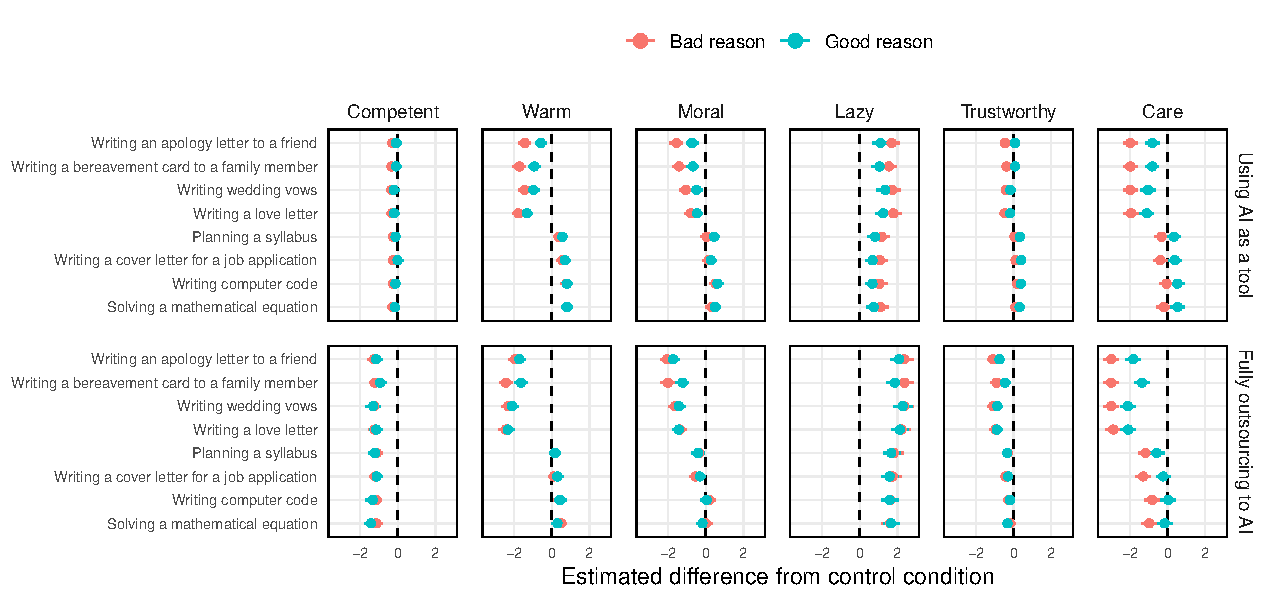
\includegraphics[keepaspectratio]{manuscript_files/figure-pdf/fig-treatments-tasks-study4-1.pdf}}
\end{center}

\vspace{-20pt}
\noindent \emph{Note.} Tasks are ordered from most social (top) to least
social (bottom) according to ratings from a pilot study. Point ranges
are differences in marginal means on a 7-point Likert scale for the bad
reason conditions (red) and good reason conditions (blue) compared to
the control condition. Upper panels refer to the tool outsourcing
conditions, and lower panels refer to the full outsourcing conditions.
Points and ranges represent posterior medians and 95\% credible
intervals, respectively.

\end{figure}

\end{landscape}

Moreover, when we delved further into the task-specific estimates, we
found that the reasons manipulation did indeed have an effect on
character evaluations for social tasks -- but not non-social tasks
(Supplementary Figure~\ref{suppfig-reasons-tasks-study4}). When writing
a bereavement card, for example, people were perceived as less warm,
less moral, lazier, and less trustworthy when they used AI to save time
compared to when they used it because they cared about doing the task
well. The same was not true for non-social tasks like writing computer
code or solving a mathematical equation.

\subsection*{Discussion}\label{discussion-3}

In Study 4, we attempted to counteract the potential perception that
outsourcing to AI reflects caring less about the task by explicitly
informing participants about the person's reason for outsourcing: they
outsourced to AI because they really cared about the task and wanted to
get it right. As well as replicating our finding that fully outsourcing
to AI is perceived more negatively than using AI as a tool, we also
found an important effect of the reasons for outsourcing, but only for
socio-relational tasks. When writing a bereavement card or an apology
letter, for example, people were perceived more negatively if they used
an AI tool to produce a quick output in a rush, rather than to ensure
they got it right. Nonetheless, for socio-relational tasks, the ``best''
use of AI in this study -- using AI as a tool because they cared about
the task and wanted to get it right --- \emph{still} led to targets
being perceived more negatively than if they had completed the task
themselves.

While we have so far shown varying evidence for three different
mechanisms that might underlie the negative perceptions of outsourcing
to AI -- effort, authenticity, and caring about the task -- it is likely
that these mechanisms are related. For example, outsourcing to AI might
indicate a lack of effort, which then might signal a lack of
authenticity and reduced care in the task, leading to negative character
evaluations. Our previous studies have been unable to test causal models
like these as we manipulated the mechanisms separately and
independently. In Study 5, therefore, we bring all three mechanisms
together and test their combined associations with character
evaluations. To do this, we focus on a single socio-relational task ---
writing a love letter --- which we elaborate for participants with a
more detailed vignette.

\section*{Study 5}\label{study-5}

\subsection*{Methods}\label{methods-4}

\subsubsection*{Participants}\label{participants-4}

We conducted a power simulation to determine our target sample size. The
simulation suggested that a sample size of 200 participants per
condition (overall \emph{n} = 600 for three conditions) would be
required to detect a small-to-medium difference between conditions
(Cohen's \emph{d} ≈ 0.30) with above 80\% power.

We recruited a convenience sample of 651 participants from the United
Kingdom through Prolific. After excluding participants who failed our
pre-treatment attention check, we were left with a final sample of 610
participants (371 female; 233 male; 4 non-binary / third gender; 2
undisclosed gender; mean age = 42.85 years). 82\% of these participants
reported having used AI tools like ChatGPT before.

\subsubsection*{Design}\label{design-4}

We randomly allocated participants into one of three conditions in a
between-subjects design: (\emph{i}) the control condition, (\emph{ii})
the tool outsourcing condition, or (\emph{iii}) the full outsourcing
condition. These conditions determined how the scenario was presented to
participants.

\subsubsection*{Procedure}\label{procedure-4}

We presented participants with a vignette about a person, Adam, who is
writing a love letter in a Valentine's Day card to his partner (see
Supplementary Materials for full vignette wording). We told participants
in each of the conditions:

\begin{itemize}
\tightlist
\item
  \emph{Control condition}: ``Adam decides to write the love letter in
  the card by himself.''
\item
  \emph{Tool outsourcing condition}: ``Adam decides to use AI to help
  write the love letter in the card. He asks ChatGPT to provide ideas,
  inspiration, and feedback, but he edits and rewrites the suggestions
  and finishes writing the love letter himself.''
\item
  \emph{Full outsourcing condition}: ``Adam decides to use AI to write
  the love letter in the card. He asks ChatGPT to write the love letter
  and copies the output word-for-word, rather than writing it himself.''
\end{itemize}

We then presented participants with the love letter that Adam wrote (in
reality, this was written by ChatGPT version 4o; see Supplementary
Materials for wording). On the following page, we asked participants
what Adam wrote and whether he used AI to help. 95\% of participants
answered both of these comprehension questions correctly.

Using 7-point Likert scales, we then asked participants how much effort
they thought Adam put into the love letter, how authentic they thought
the love letter was, how much they thought Adam cared about the love
letter, and the same five character evaluations as in our previous
studies. In additional free response questions, we asked participants to
explain how they felt towards Adam and how they would feel if they were
Adam's partner. Finally, we asked participants several questions about
AI tools like ChatGPT.

\subsubsection*{Pre-registration}\label{pre-registration-4}

We pre-registered the study on the Open Science Framework
(\url{https://osf.io/ac9g3/?view_only=912d9b57023d49baa87eea999574f0ce}).

\subsubsection*{Statistical Analysis}\label{statistical-analysis-4}

We fitted two Bayesian regression models to the data. The first model
was a multivariate cumulative-link ordinal model including all Likert
scales as separate response variables. The second model was a path model
capturing the effect of outsourcing on character evaluations, both
directly and indirectly through perceptions of effort, authenticity, and
care. In this second model, we included ordinal predictors as monotonic
effects and modelled the five character evaluations as a single latent
variable. We used regularising priors for all parameters to impose
conservatism on parameter estimates. All models converged normally
(\(\hat{R}\) ≤ 1.01).

\subsection*{Results}\label{results-4}

Across all measures, we found that outsourcing the love letter to AI was
perceived more negatively compared to the control condition and that
fully outsourcing to AI was perceived more negatively than using AI as a
collaborative tool (Figure~\ref{fig-treatments-study5};
Table~\ref{tbl-treatment-diffs-study5}). Not only did outsourcing the
love letter lead to more negative character evaluations, but outsourcing
to AI was also seen as less effortful, less authentic, and indicative of
caring less about the task.

\begin{figure}[!htbp]

{\caption{{Perceptions of the Person and the Love Letter in Study
5}{\label{fig-treatments-study5}}}}

\begin{center}
\pandocbounded{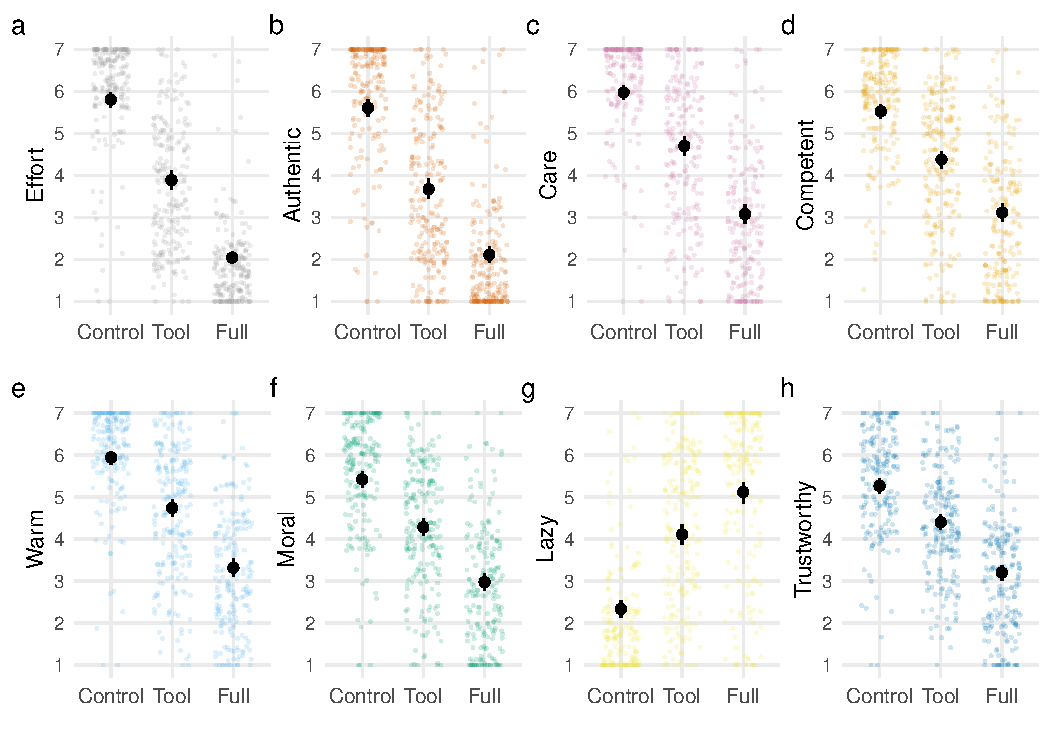
\includegraphics[keepaspectratio]{manuscript_files/figure-pdf/fig-treatments-study5-1.pdf}}
\end{center}

\vspace{-20pt}
\noindent \emph{Note.} Participants in the control, tool outsourcing,
and full outsourcing conditions rated (a) the amount of effort put into
the love letter, (b) how authentic the love letter was, (c) how much the
person cared about the love letter, and (d-h) five character evaluation
measures. Coloured points represent participant responses to the
questions, jittered for easier viewing. Black points are estimated
marginal means from the fitted model. Black points and line ranges
represent posterior medians and 95\% credible intervals, respectively.

\end{figure}

\begin{landscape}

\begin{table}

{\caption{{Pairwise Contrasts in Study 5
\vspace{20pt}}{\label{tbl-treatment-diffs-study5}}}
\vspace{-20pt}}

\begingroup\fontsize{8}{10}\selectfont

\begin{tabular}{lllllllll}
\toprule
\multicolumn{1}{c}{ } & \multicolumn{8}{c}{Response} \\
\cmidrule(l{3pt}r{3pt}){2-9}
  & Effort & Authentic & Care & Competent & Warm & Moral & Lazy & Trustworthy\\
\midrule
Tool - Control & -1.91 [-2.18 -1.64] & -1.94 [-2.23 -1.61] & -1.27 [-1.54 -1.00] & -1.15 [-1.40 -0.89] & -1.20 [-1.45 -0.95] & -1.14 [-1.39 -0.88] & 1.77 [1.47 2.07] & -0.86 [-1.11 -0.62]\\
Full - Control & -3.76 [-3.98 -3.52] & -3.50 [-3.77 -3.22] & -2.90 [-3.16 -2.63] & -2.41 [-2.67 -2.14] & -2.62 [-2.88 -2.37] & -2.44 [-2.71 -2.17] & 2.78 [2.47 3.09] & -2.07 [-2.30 -1.82]\\
Full - Tool & -1.85 [-2.11 -1.58] & -1.56 [-1.87 -1.26] & -1.63 [-1.93 -1.31] & -1.26 [-1.55 -0.97] & -1.42 [-1.72 -1.12] & -1.31 [-1.60 -1.02] & 1.01 [0.65 1.35] & -1.20 [-1.45 -0.95]\\
\bottomrule
\end{tabular}
\endgroup{}\vspace{40pt}

\vspace{-20pt}
\noindent \emph{Note.} Numbers reflect differences in marginal means on
a 7-point Likert scale. Main numbers are posterior medians, numbers in
the square brackets are 95\% credible intervals.

\end{table}

\end{landscape}

Exploratory text analysis of participants' free responses supported this
quantitative pattern (see Supplementary Materials for methodology and
Supplementary Table~\ref{supptbl-text-analysis-study5} for results).
When comparing word frequencies between conditions, we found that Adam
was more likely to be described as ``lazy'' and less likely to be
described as ``caring'', ``thoughtful'', and ``genuine'' in both
outsourcing conditions compared to the control condition. Adam was also
more likely to be described as ``romantic'' and as someone who ``loves''
his partner when he used AI as a collaborative tool, compared to when he
fully outsourced the love letter to AI.

When we included all the variables in a single path model, we found that
outsourcing influenced character evaluations both directly and
indirectly through our proposed mechanisms
(Figure~\ref{fig-path-model-study5}). The indirect effects showed that
people perceived outsourced work as less effortful, and less effortful
work was seen as less authentic and indicating less care about the task.
In turn, less authenticity and care were associated with more negative
evaluations of the person. Effort itself was not directly related to
character evaluations, suggesting that effort works solely through
perceptions of authenticity and care.

\begin{figure}[!htbp]

{\caption{{Path Model in Study 5}{\label{fig-path-model-study5}}}}

\begin{center}
\pandocbounded{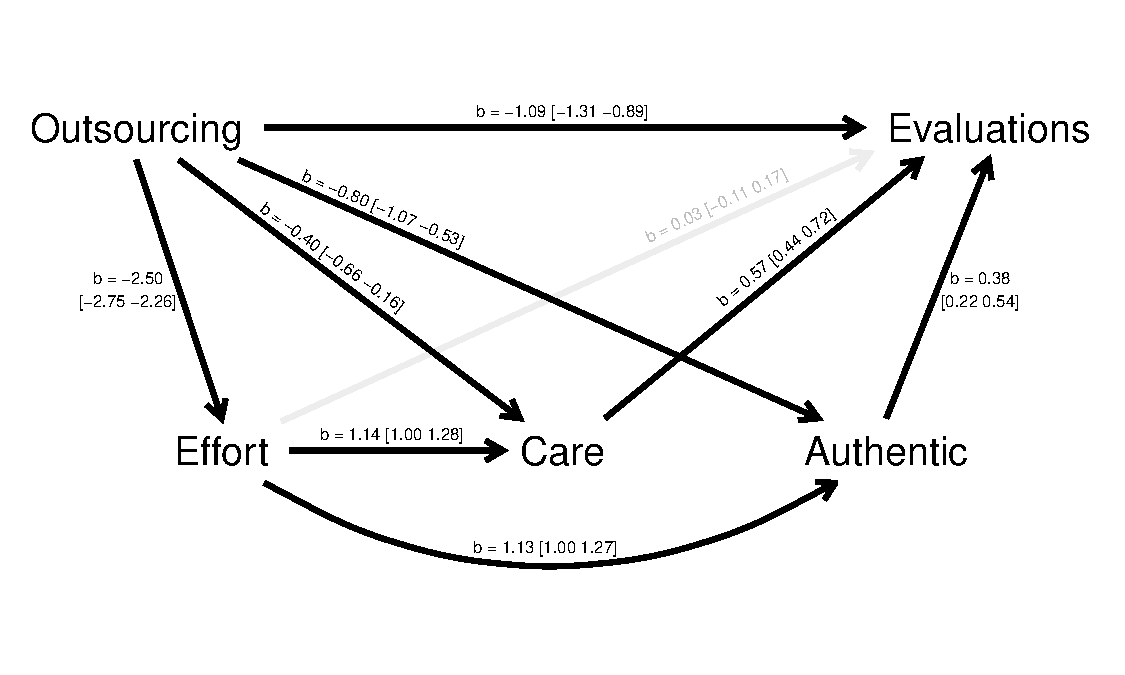
\includegraphics[keepaspectratio]{manuscript_files/figure-pdf/fig-path-model-study5-1.pdf}}
\end{center}

\vspace{-20pt}
\noindent \emph{Note.} All predictors were modelled as monotonic
effects, such that parameters can be interpreted as the expected average
difference between two adjacent categories of the ordinal predictor on
the logit scale. The ``evaluations'' outcome variable was modelled as a
single latent variable with loadings from all five character evaluations
(competence, warmth, morality, laziness, and trustworthiness).

\end{figure}

\section*{General Discussion}\label{general-discussion}

The release of openly available generative AI LLMs has changed lives,
promising to let people do more tasks, more efficiently, and perhaps to
do so better than they could alone. People can --- and \emph{do} --- use
AI tools like ChatGPT to, for example, create dinner recipes, assist
with coding, and even write job applications
(\citeproc{ref-UKGov2024}{Department for Science, Innovation \&
Technology, 2024}). But it is not only such routine, everyday, and
non-social tasks that AI now ``assists'' with. People can use AI for a
seemingly endless range of social tasks too, from crafting apology
letters to writing condolences to even writing wedding vows. In this
paper, across five pre-registered experiments, we show how --- and why
--- AI-outsourcing shapes perceptions of others in a world where
outsourcing has never been easier and cheaper.

In Study 1, we showed that people who outsourced tasks to AI were
perceived more negatively than people who completed the tasks by
themselves. These negative impressions were particularly strong for
people who used AI to complete socio-relational tasks, such as writing a
love letter or writing wedding vows, and for people who copied the
model's first output verbatim without acknowledging their reliance on
AI. Moreover, these negative perceptions were found even for the ``best
case'' of openly acknowledging the use of AI as a collaborative tool. In
Study 2, we showed that people perceive both the outsourcer and the
outsworked work more negatively, with outsourced work perceived as less
meaningful, less authentic, and less reward-worthy than ostensibly
human-generated writing. In Study 3, we showed that while it matters
whether people spent time crafting the AI prompts or simply gave a
rushed initial prompt, even expending effort into crafting the best
prompts was still not enough to counteract the negative effects from
using AI. In Study 4, we explored the potential role of inferred
importance and found that while explicitly telling participants that the
person used AI because they cared about the task reduced negative
perceptions for social tasks, it was still not enough to eliminate
negative perceptions completely. In Study 5, we showed that a perceived
lack of effort is taken to signal both a lack of authenticity and lack
of importance attached to the task, and these independently influenced
character judgments above and beyond the effect of effort.

Our findings extend work on the moralisation of effort. Studies have
shown that people inherently value effort and perceive displays of
effort as costly signals of one's moral character and cooperative intent
(\citeproc{ref-Celniker2023}{Celniker et al., 2023}). And yet it has
remained unclear how we might view others who outsource to AI; how these
effects might vary based on how socio-relational the task is; how
different ways of outsourcing influence perceptions; how outsourcing has
different effects on different kinds of social perceptions; and why
exactly effort has the effects that it does. Across our studies, we
provide new insight into all of these questions. In line with previous
work on the importance of effort, we show that people negatively judge
those who outsource to AI. We show that the type of task does matter,
whereby outsourcing to AI for socio-relational tasks leads to
particularly negative perceptions. We show that different ways of
outsourcing lead to differences in the degree of negative perceptions
but that, critically, even outsourcing to AI in the ``best'' way (e.g.,
using it as a tool and finishing the work oneself while being honest
about the AI use) is still not enough to eliminate the negative
consequences. We show that negative perceptions from outsourcing tended
to go together, even if outsourcing on social tasks led to particularly
negative effects on warmth and morality traits. And finally, we provide
further insight into why effort matters. The reduced effort from
outsourcing socio-relational tasks to AI signals that the work is less
authentically one's own and that the person cares less about the task
(and therefore, perhaps, the relationship). The lack of a direct effect
of perceived effort in our path model showed that it is inferences of
authenticity and care, rather than perceived effort per se, that are
associated with negative character evaluations. As a participant in our
final study put it: ``\emph{If he really cared, he would have just done
it by himself from scratch}'' (female, 25 years old).

Our findings cohere with the philosophical idea that there is value in
\emph{how} a task was done, and not merely \emph{whether} it was done
(\citeproc{ref-Aristotle2009}{Aristotle, 2009};
\citeproc{ref-Goodman2010}{Goodman, 2010};
\citeproc{ref-Hursthouse2023}{Hursthouse \& Pettigrove, 2023};
\citeproc{ref-Stohr2006}{Stohr, 2006}). For many socio-relational tasks,
it might seem that part of the constitutive action is the \emph{process}
by which it occurs: an apology that does not contain a genuine
reflection and commitment to do better, rather than just the words ``I
am sorry'', might not seem to be an apology at all. In contrast, for
many of the non-social tasks, it is easier to distinguish the importance
of the process from the outcome. In this way, our work suggests that
people rarely adopt a purely utilitarian perspective in which outcomes
are the sole determinant (\citeproc{ref-Everett2020}{Everett \& Kahane,
2020}; \citeproc{ref-Kahane2018}{Kahane et al., 2018}). Instead, their
judgments cohere more with ideas from virtue ethics about the importance
of \emph{doing} (\citeproc{ref-Hursthouse2023}{Hursthouse \& Pettigrove,
2023}; \citeproc{ref-Stohr2006}{Stohr, 2006}). Outsourcing to AI --
especially for social tasks --- may allow us to produce similar outputs,
but by severing the outcome from the practice of doing, it may risk the
development and maintenance of our human virtues
(\citeproc{ref-Vallor2015}{Vallor, 2015},
\citeproc{ref-Vallor2024}{2024}).

AI is often being marketed as being able to help us to do more and more
tasks, promising gains of efficiency that align with societal incentives
for ``hacks'' that encourage people to do more-and-more with less energy
and effort. Our work, however, highlights that when it comes to our
psychology, efficiency is not the only currency. Instead,
\emph{in}efficiency can sometimes pay off more, especially for social
tasks. By expending effort themselves instead of outsourcing to AI,
people are able to signal authenticity and care for the task, and this
can lead to better reputations (see also
\citeproc{ref-Celniker2023}{Celniker et al., 2023}). Correspondingly,
expending effort, even ``unnecessarily'', is not as irrational, biased,
or suboptimal as we might think from a utilitarian perspective in which
outcomes are the only things that matter. Instead, it is precisely this
inefficiency that helps people signal things that they care about and
connect with others, thereby arguably reflecting a deeply rational
reflection of virtues and the importance of social ties
(\citeproc{ref-Everett2016}{Everett et al., 2016}).

Most speculatively, our results on the negative effects of
AI-outsourcing on character judgments highlight potential risks in how
increased use of AI could lead to negative consequences for social ties,
especially if people start to assume, by default, that others are using
AI for the kind of tasks that matter. Sociologists have highlighted
concerns about the negative effects that outsourcing to AI can have on
our ``connective labour'', arguing that while AI can enhance certain
tasks, it cannot replicate the depth of human relationships essential
for effective caregiving, education, and support
(\citeproc{ref-Pugh2024}{Pugh, 2024}). Similar arguments have been made
about the risks of outsourcing empathy to AI
(\citeproc{ref-Landes2025}{Landes \& Everett, 2025}). In this way, the
rapid move towards using AI for more and more tasks could have serious
and unintended consequences on the way we connect with one another,
serving to further weaken the social ties that bind us into a community.

\subsection*{Limitations and Directions for Future
Research}\label{limitations-and-directions-for-future-research}

The studies in this paper are not without their limitations. While we
included a range of different socio-relational and professional tasks in
an effort to improve the generalisability of our findings across
domains, it would be interesting for future work to additionally explore
the generalisability and variability of our findings across countries
with different AI infrastructures and readiness levels
(\citeproc{ref-OxfordInsights}{Oxford Insights, 2024};
\citeproc{ref-TortoiseMedia}{Tortoise Media, 2024}) and over time as AI
use becomes more commonplace. By focusing on generalisability across
various real-world tasks in which people outsource, it could also be
argued that our design lacks the richness of information in extended
vignettes that might influence character evaluations. While we have
advanced previous research in highlighting the ways in which effort
influences perceptions of authenticity and care, it will be interesting
for future research to delve deeper into these mechanisms, both
philosophically and psychologically: \emph{why} is it that the perceived
care for the task matters, and what are the boundary conditions of these
effects? Finally, while we have demonstrated negative perceptions of
outsourcing in this paper, it will be important for future research to
explore when people might deem outsourcing to AI as acceptable or even
preferable. Several of the participants in our final study expressed in
their free responses that they would have been okay with Adam using AI
to write the love letter if he was not a confident writer or had a
learning difficulty that made writing challenging, such as dyslexia. In
line with this, some research has found that people are more accepting
of cognition-enhancing technologies and drugs when they are used to
repair cognitive functions, rather than to enhance cognitive functions
beyond ``normal'' levels (\citeproc{ref-Medaglia2019}{Medaglia et al.,
2019}; \citeproc{ref-Rudski2014}{Rudski, 2014}). Future research should
explore whether negative perceptions of outsourcing persist when AI is
used in a reparative way.

\subsection*{Conclusions}\label{conclusions}

To conclude, across five pre-registered studies, we have demonstrated
negative perceptions of outsourcing to AI. Our participants perceived
individuals who outsource tasks to AI more negatively across a range of
character dimensions and perceived outsourced work as less meaningful
and authentic. Negative perceptions were particularly strong for
socio-relational tasks, such as writing wedding vows, and were
compounded when the outsourcer copied the AI's output verbatim and did
not honestly acknowledge their use of AI. These findings connect with
broader debates about the importance of \emph{doing} in social
relationships, and highlight that for many tasks -- especially those
that are more socio-relational -- it might be better to move away from a
focus on making things more efficient at all costs and instead bring
back a recognition of the power of \emph{in}efficiency. Doing something
oneself, even if AI could do it quicker and easier, signals one that is
authentic and cares about the task and therefore can help bind us
together. In a world of algorithm-mediated interactions, AI is no
substitute for investing effort into our interpersonal relationships.

\newpage
\nolinenumbers

\section*{Acknowledgements}\label{acknowledgements}

This work was generously supported by funding from REDACTED.

\section*{Data and Code Availability}\label{data-and-code-availability}

All data and original code can be found here:
\url{https://osf.io/ac9g3/?view_only=912d9b57023d49baa87eea999574f0ce}.

\section*{Statement of Interests}\label{statement-of-interests}

The authors have no conflicts of interest to disclose.

\newpage

\section*{References}\label{references}

\phantomsection\label{refs}
\begin{CSLReferences}{1}{0}
\bibitem[\citeproctext]{ref-Abele2021}
Abele, A. E., Ellemers, N., Fiske, S. T., Koch, A., \& Yzerbyt, V.
(2021). Navigating the social world: Toward an integrated framework for
evaluating self, individuals, and groups. \emph{Psychological Review},
\emph{128}(2), 290--314. \url{https://doi.org/10.1037/rev0000262}

\bibitem[\citeproctext]{ref-Allaire2024}
Allaire, J. J., Teague, C., Scheidegger, C., Xie, Y., Dervieux, C., \&
Woodhull, G. (2024). \emph{{Quarto}} (Version 1.7.23) {[}Computer
software{]}. \url{https://doi.org/10.5281/zenodo.5960048}

\bibitem[\citeproctext]{ref-Anderson2025}
Anderson, L. (2025). \emph{How are students using {ChatGPT}? For
therapy, breakups, and even texting friends}. Teen Vogue.
\url{https://www.teenvogue.com/story/how-students-using-chatgpt-therapy-breakups}

\bibitem[\citeproctext]{ref-Aristotle2009}
Aristotle. (2009). \emph{The {Nicomachean} ethics {(D. Ross \& L. Brown,
Translators)}}. Oxford University Press.

\bibitem[\citeproctext]{ref-Burkner2017}
Bürkner, P.-C. (2017). {brms}: An {R} package for {Bayesian} multilevel
models using {Stan}. \emph{Journal of Statistical Software},
\emph{80}(1), 1--28. \url{https://doi.org/10.18637/jss.v080.i01}

\bibitem[\citeproctext]{ref-Celniker2023}
Celniker, J. B., Gregory, A., Koo, H. J., Piff, P. K., Ditto, P. H., \&
Shariff, A. F. (2023). The moralization of effort. \emph{Journal of
Experimental Psychology: General}, \emph{152}(1), 60--79.
\url{https://doi.org/10.1037/xge0001259}

\bibitem[\citeproctext]{ref-Cubitt2011}
Cubitt, R. P., Drouvelis, M., Gächter, S., \& Kabalin, R. (2011). Moral
judgments in social dilemmas: How bad is free riding? \emph{Journal of
Public Economics}, \emph{95}(3), 253--264.
\url{https://doi.org/10.1016/j.jpubeco.2010.10.011}

\bibitem[\citeproctext]{ref-UKGov2024}
Department for Science, Innovation \& Technology. (2024). \emph{Public
attitudes to data and {AI}: Tracker survey ({Wave 4}) report}.
\url{https://www.gov.uk/government/publications/public-attitudes-to-data-and-ai-tracker-survey-wave-4/public-attitudes-to-data-and-ai-tracker-survey-wave-4-report}

\bibitem[\citeproctext]{ref-Earp2024}
Earp, B. D., Porsdam Mann, S., Liu, P., Hannikainen, I., Khan, M. A.,
Chu, Y., \& Savulescu, J. (2024). Credit and blame for AI-generated
content: Effects of personalization in four countries. \emph{Annals of
the New York Academy of Sciences}, \emph{1542}(1), 51--57.
\url{https://doi.org/10.1111/nyas.15258}

\bibitem[\citeproctext]{ref-Everett2020}
Everett, J. A., \& Kahane, G. (2020). Switching tracks? Towards a
multidimensional model of utilitarian psychology. \emph{Trends in
Cognitive Sciences}, \emph{24}(2), 124--134.
\url{https://doi.org/10.1016/j.tics.2019.11.012}

\bibitem[\citeproctext]{ref-Everett2016}
Everett, J. A., Pizarro, D. A., \& Crockett, M. J. (2016). Inference of
trustworthiness from intuitive moral judgments. \emph{Journal of
Experimental Psychology: General}, \emph{145}(6), 772--787.
\url{https://doi.org/10.1037/xge0000165}

\bibitem[\citeproctext]{ref-Fiske1992}
Fiske, A. P. (1992). The four elementary forms of sociality: Framework
for a unified theory of social relations. \emph{Psychological Review},
\emph{99}(4), 689--723. \url{https://doi.org/10.1037/0033-295X.99.4.689}

\bibitem[\citeproctext]{ref-Fiske2007}
Fiske, S. T., Cuddy, A. J., \& Glick, P. (2007). Universal dimensions of
social cognition: Warmth and competence. \emph{Trends in Cognitive
Sciences}, \emph{11}(2), 77--83.
\url{https://doi.org/10.1016/j.tics.2006.11.005}

\bibitem[\citeproctext]{ref-Goodman2010}
Goodman, R. (2010). Cognitive enhancement, cheating, and accomplishment.
\emph{Kennedy Institute of Ethics Journal}, \emph{20}(2), 145--160.
\url{https://doi.org/10.1353/ken.0.0309}

\bibitem[\citeproctext]{ref-Goodwin2014}
Goodwin, G. P., Piazza, J., \& Rozin, P. (2014). Moral character
predominates in person perception and evaluation. \emph{Journal of
Personality and Social Psychology}, \emph{106}(1), 148--168.
\url{https://doi.org/10.1037/a0034726}

\bibitem[\citeproctext]{ref-Heider1958}
Heider, F. (1958). \emph{The psychology of interpersonal relations}.
John Wiley \& Sons Inc. \url{https://doi.org/10.1037/10628-000}

\bibitem[\citeproctext]{ref-Hursthouse2023}
Hursthouse, R., \& Pettigrove, G. (2023). Virtue ethics. In E. N. Zalta
\& U. Nodelman (Eds.), \emph{The {Stanford} encyclopedia of philosophy}.
\url{https://plato.stanford.edu/archives/fall2023/entries/ethics-virtue/}

\bibitem[\citeproctext]{ref-Kahane2018}
Kahane, G., Everett, J. A., Earp, B. D., Caviola, L., Faber, N. S.,
Crockett, M. J., \& Savulescu, J. (2018). Beyond sacrificial harm: A
two-dimensional model of utilitarian psychology. \emph{Psychological
Review}, \emph{125}(2), 131--164.
\url{https://doi.org/10.1037/rev0000093}

\bibitem[\citeproctext]{ref-Kerr1983}
Kerr, N. L. (1983). Motivation losses in small groups: A social dilemma
analysis. \emph{Journal of Personality and Social Psychology},
\emph{45}(4), 819--828. \url{https://doi.org/10.1037/0022-3514.45.4.819}

\bibitem[\citeproctext]{ref-Kruger2004}
Kruger, J., Wirtz, D., Van Boven, L., \& Altermatt, T. W. (2004). The
effort heuristic. \emph{Journal of Experimental Social Psychology},
\emph{40}(1), 91--98.
\url{https://doi.org/10.1016/S0022-1031(03)00065-9}

\bibitem[\citeproctext]{ref-Landau2021}
Landau, W. M. (2021). The targets {R} package: A dynamic {M}ake-like
function-oriented pipeline toolkit for reproducibility and
high-performance computing. \emph{Journal of Open Source Software},
\emph{6}(57), 2959. \url{https://doi.org/10.21105/joss.02959}

\bibitem[\citeproctext]{ref-Landes2025}
Landes, E., \& Everett, J. A. C. (2025). \emph{AI should develop human
empathy, not replace it}. PsyArXiv.
\url{https://doi.org/10.31234/osf.io/y3qzu_v1}

\bibitem[\citeproctext]{ref-Liu2024}
Liu, B., Kang, J., \& Wei, L. (2024). Artificial intelligence and
perceived effort in relationship maintenance: Effects on relationship
satisfaction and uncertainty. \emph{Journal of Social and Personal
Relationships}, \emph{41}(5), 1232--1252.
\url{https://doi.org/10.1177/02654075231189899}

\bibitem[\citeproctext]{ref-Malle2022}
Malle, B. F. (2022). Attribution theories. In \emph{Theories in social
psychology, second edition} (pp. 93--120). John Wiley \& Sons, Ltd.
\url{https://doi.org/10.1002/9781394266616.ch4}

\bibitem[\citeproctext]{ref-Medaglia2019}
Medaglia, J. D., Yaden, D. B., Helion, C., \& Haslam, M. (2019). Moral
attitudes and willingness to enhance and repair cognition with brain
stimulation. \emph{Brain Stimulation}, \emph{12}(1), 44--53.
\url{https://doi.org/10.1016/j.brs.2018.09.014}

\bibitem[\citeproctext]{ref-miramar0}
miramar0. (2024). \emph{My (30F) husband (36M) used {AI} to write his
vows. How do {I} approach him about this?} {[}Online forum post{]}.
Reddit.
\url{https://www.reddit.com/r/relationship_advice/comments/1d9tw9j/my_30f_husband_36m_used_ai_to_write_his_vows_how/}

\bibitem[\citeproctext]{ref-Newman2019}
Newman, G. E. (2019). The psychology of authenticity. \emph{Review of
General Psychology}, \emph{23}(1), 8--18.
\url{https://doi.org/10.1037/gpr0000158}

\bibitem[\citeproctext]{ref-Noy2023}
Noy, S., \& Zhang, W. (2023). Experimental evidence on the productivity
effects of generative artificial intelligence. \emph{Science},
\emph{381}(6654), 187--192.
\url{https://doi.org/10.1126/science.adh2586}

\bibitem[\citeproctext]{ref-OxfordInsights}
Oxford Insights. (2024). \emph{Government {AI} readiness index}.
\url{https://oxfordinsights.com/ai-readiness/ai-readiness-index/}

\bibitem[\citeproctext]{ref-Pedersen2025}
Pedersen, T. L. (2025). \emph{{patchwork}: The composer of plots}.
\url{https://patchwork.data-imaginist.com}

\bibitem[\citeproctext]{ref-Pugh2024}
Pugh, A. J. (2024). \emph{The last human job: The work of connecting in
a disconnected world}. Princeton University Press.

\bibitem[\citeproctext]{ref-RCoreTeam}
R Core Team. (2022). \emph{R: A language and environment for statistical
computing}. R Foundation for Statistical Computing.
\url{https://www.R-project.org/}

\bibitem[\citeproctext]{ref-Roth2025}
Roth, L. H. O., \& Tissot, T. (2025). \emph{A costly co-pilot? {AI}
usage signals reduced morality via effort perceptions}. OSF Preprints.
\url{https://doi.org/10.31219/osf.io/vwxgz_v1}

\bibitem[\citeproctext]{ref-Rudski2014}
Rudski, J. M. (2014). A comparison of attitudes toward pharmacological
treatment versus enhancement under competitive and noncompetitive
conditions. \emph{AJOB Empirical Bioethics}, \emph{5}(2), 80--90.
\url{https://doi.org/10.1080/23294515.2013.850122}

\bibitem[\citeproctext]{ref-Stohr2006}
Stohr, K. (2006). Contemporary virtue ethics. \emph{Philosophy Compass},
\emph{1}(1), 22--27.
\url{https://doi.org/10.1111/j.1747-9991.2006.00004.x}

\bibitem[\citeproctext]{ref-Tait2024}
Tait, A. (2024). \emph{{M}y boyfriend sent me a heartfelt message - then
{I} learned he'd used {ChatGPT}}. The i Paper.
\url{https://inews.co.uk/inews-lifestyle/boyfriend-sent-heartfelt-message-learned-chatgpt-3413336}

\bibitem[\citeproctext]{ref-TortoiseMedia}
Tortoise Media. (2024). \emph{The global {AI} index}.
\url{https://www.tortoisemedia.com/data/global-ai}

\bibitem[\citeproctext]{ref-Vallor2015}
Vallor, S. (2015). Moral deskilling and upskilling in a new machine age:
Reflections on the ambiguous future of character. \emph{Philosophy \&
Technology}, \emph{28}, 107--124.
\url{https://doi.org/10.1007/s13347-014-0156-9}

\bibitem[\citeproctext]{ref-Vallor2024}
Vallor, S. (2024). \emph{The {AI} mirror: How to reclaim our humanity in
an age of machine thinking}. Oxford University Press.
\url{https://doi.org/10.1093/oso/9780197759066.001.0001}

\bibitem[\citeproctext]{ref-Wickham2016}
Wickham, H. (2016). \emph{{ggplot2}: Elegant graphics for data
analysis}. Springer-Verlag New York. \url{https://ggplot2.tidyverse.org}

\end{CSLReferences}

\newpage

\vspace*{30mm}

\section*{Supplementary Materials}\label{supplementary-materials}

\setcounter{page}{1}
\begin{center}
Negative Perceptions of Outsourcing to Artificial Intelligence \\
AUTHORS REDACTED \\
AFFILIATION REDACTED
\end{center}
\vspace*{30mm}
\tableofcontents
\newpage

\section{Pilot Study 1}\label{pilot-study-1}

\subsection*{Methods}\label{methods-5}

\subsubsection*{Participants}\label{participants-5}

We recruited a convenience sample of 200 participants from the United
Kingdom through Prolific. After excluding participants who failed our
pre-treatment attention check, we were left with a final sample of 186
participants (118 female; 67 male; 1 non-binary / third gender; 0
undisclosed gender; mean age = 38.99 years).

\subsubsection*{Procedure}\label{procedure-5}

We presented participants with six different tasks ``that people might
perform in their daily lives''. The six tasks were randomly drawn from a
larger set of 20 tasks (see Supplementary Table~\ref{supptbl-tasks} for
the full list of tasks). For each task, we asked participants the
following questions on 7-point Likert scales:

\begin{itemize}
\tightlist
\item
  Is this a social task?
\item
  Does this task require social skills?
\item
  Does this task impact other people?
\item
  How important are the consequences of this task?
\item
  How important is it that effort goes into this task?
\item
  How important is it that others see the effort that goes into this
  task?
\end{itemize}

\subsubsection*{Statistical Analysis}\label{statistical-analysis-5}

We fitted a Bayesian multivariate multilevel cumulative-link ordinal
model to the data using the \emph{brms} R package. We modelled each task
evaluation as a separate response variable and included correlated
varying intercepts for participants and tasks. We used regularising
priors for all parameters to impose conservatism on parameter estimates
(see Supplementary Materials for full model specification). The model
converged normally (\(\hat{R}\) ≤ 1.01).

\subsection*{Results}\label{results-5}

We found that participants' responses to all six questions tended to be
positively correlated. For example, tasks rated as more social were also
rated as requiring more social skills (see
Supplementary Figure~\ref{suppfig-tasks-correlations}). Estimated
averages and rankings for the 20 tasks across each of the questions can
be found in Supplementary Figures \ref{suppfig-tasks-social} --
\ref{suppfig-tasks-extrinsiceffort}.

\newpage

\section{Pilot Study 2}\label{pilot-study-2}

\subsection*{Methods}\label{methods-6}

\subsubsection*{Participants}\label{participants-6}

We conducted a power simulation to determine our target sample size. The
simulation suggested that a sample size of 150 participants per
condition (overall \emph{n} = 450 for three conditions) would be
required to detect a small difference between conditions (Cohen's
\emph{d} ≈ 0.20) with above 80\% power.

We recruited a convenience sample of 500 participants from the United
Kingdom through Prolific. After excluding participants who failed our
pre-treatment attention check, we were left with a final sample of 466
participants (292 female; 169 male; 4 non-binary / third gender; 1
undisclosed gender; mean age = 42.32 years). 73\% of these participants
reported having used ChatGPT before.

\subsubsection*{Design}\label{design-5}

We randomly allocated participants into one of three conditions in a
between-subjects design: (\emph{i}) the control condition, (\emph{ii})
the AI outsourcing condition, or (\emph{iii}) the human outsourcing
condition. These conditions determined how scenarios were presented to
participants.

\subsubsection*{Procedure}\label{procedure-6}

We presented participants with six scenarios. Each scenario described a
person completing a task, such as writing computer code or writing a
love letter. The six tasks were randomly drawn from a larger set of 20
tasks (see Supplementary Table~\ref{supptbl-tasks} for the full list of
tasks). For each scenario, we told participants:

\begin{itemize}
\tightlist
\item
  \emph{Control condition}: ``In order to complete this task, {[}the
  person{]} works on it by themselves from start to finish.''
\item
  \emph{AI outsourcing condition}: ``In order to complete this task,
  {[}the person{]} gets the AI tool ChatGPT to do it for them.''
\item
  \emph{Human outsourcing condition}: ``In order to complete this task,
  {[}the person{]} gets someone else to do it for them.''
\end{itemize}

We then asked participants how well each of the following words
described the person in the scenario: competent, warm, moral, lazy, and
trustworthy. Participants answered these questions on 7-point Likert
scales, ranging from ``does not describe {[}the person{]} well'' to
``describes {[}the person{]} extremely well''.

After the six scenarios, we asked participants several questions about
the AI tool ChatGPT, including their familiarity with ChatGPT, whether
they had used ChatGPT before, how frequently they used ChatGPT, and how
trustworthy they thought ChatGPT was.

\subsubsection*{Pre-registration}\label{pre-registration-5}

We pre-registered the study on the Open Science Framework
(\url{https://osf.io/xhmzk/?view_only=a4da193574d7410ba4d2aa3945a28b05}).

\subsubsection*{Statistical Analysis}\label{statistical-analysis-6}

We fitted Bayesian multivariate multilevel cumulative-link ordinal
models to the data using the \emph{brms} R package. We modelled each
character evaluation -- competence, warmth, morality, laziness, and
trustworthiness -- as a separate response variable and included fixed
effects for conditions, varying intercepts for participants, and varying
intercepts and slopes for tasks. We used regularising priors for all
parameters to impose conservatism on parameter estimates (see
Supplementary Materials for full model specifications). All models
converged normally (\(\hat{R}\) ≤ 1.01).

\subsection*{Results}\label{results-6}

We found that people who outsourced tasks to AI or other humans were
perceived more negatively than people who completed the tasks themselves
(Supplementary Figure~\ref{suppfig-treatments-pilotstudy2}). In
particular, people who outsourced were perceived as lazier and less
competent, with smaller yet detectable differences for perceptions of
warmth, morality, and trustworthiness
(Supplementary Table~\ref{supptbl-treatment-diffs-pilotstudy2}). Across
all measures, outsourcing to other humans was perceived more negatively
than outsourcing to AI.

We found that the effects of outsourcing varied across the different
tasks, especially for perceptions of warmth and morality
(Supplementary Figure~\ref{suppfig-treatments-by-task-pilotstudy2}). For
example, people were perceived as less warm if they outsourced writing a
love letter, but not if they outsourced writing computer code.
Similarly, people were perceived as less moral if they outsourced
writing an apology letter to a friend, but not if they outsourced
writing a dinner recipe. By contrast, the effects of outsourcing on
competence, laziness, and trustworthiness were more consistent across
tasks.

To determine the factors that predict variation across tasks, we
incorporated ratings of tasks from the first pilot study. Participants
were asked to rate the 20 tasks on several features: whether the task is
social, requires social skills, impacts others, has important
consequences, and requires effort. All of these features predicted
stronger causal effects of outsourcing compared to control
(Supplementary Figures \ref{suppfig-interactions-pilotstudy2} and
\ref{suppfig-interaction-pars-pilotstudy2}). In other words, outsourcing
to AI or other humans is perceived more negatively for tasks that have
these features, compared to tasks without these features.

\newpage

\section{Vignette Wording in Study 5}\label{vignette-wording-in-study-5}

\noindent We presented participants in Study 5 with the following
vignette text:

\begin{quote}
Adam has been dating his partner for almost a year, and Valentine's Day
is coming up. He knows that many people exchange a card on Valentine's
Day containing a love letter to their partner, and he decides to send a
love letter to his partner too.

This year, Adam has been closely following developments in technology
and has read of people using AI tools like ChatGPT for things like this,
either using it to help with writing or getting AI to do the task
completely.
\end{quote}

\noindent This was followed by the manipulation text (see main text).
Participants were then presented with the love letter that Adam
ostensibly wrote, which was held constant across conditions:

\begin{quote}
Happy Valentine's Day, my love.

I don't think I tell you enough just how much you mean to me. Being with
you feels like breathing a little easier, like the world is a bit softer
just because you're in it. You make the everyday feel special, and
somehow you always know how to calm my nerves or make me laugh at just
the right moment. I feel like myself with you -- maybe even a better
version of myself -- and that's such a rare and beautiful thing.

I'm so grateful for you -- for the way you listen, the way you love, the
way you show up, even in the small ways. I hope you know that no matter
what, I'm always in your corner. I can't wait to keep making memories
together, whether we're off on some adventure or just curled up on the
couch. I love you more than I can really put into words, but I promise
I'll spend every day trying.

Yours,

Adam
\end{quote}

\newpage

\section{Methods for Text Analysis in Study
5}\label{methods-for-text-analysis-in-study-5}

To generate frequency lists for each experimental condition in Study 5,
we created three documents containing the raw text submissions to the
open-ended question ``In your own words, describe how you feel about
Adam and why''. Each raw text submission was paired with a numbered text
ID column. The number of submissions was roughly equivalent across
conditions: the control condition (N = 196), the tool outsourcing
condition (N = 215), and the full outsourcing condition (N = 202).

All text processing was conducted using the Basic Unit-Transposable Text
Experimentation Resource (BUTTER; Version 0.9.4.1; Boyd, 2019). To
prepare the data, each CSV file was converted into a folder containing
individual text files -- one per submission -- using two plugins:
\emph{Read Text from CSV} (Version 1.0.2) and \emph{Save .txt Files to
Folder} (Version 1.0.6). The settings for \emph{Read Text from CSV} were
as follows: file encoding = UTF-8, row identifier = ID, text column =
Text, CSV delimiter = , and CSV quote = ``.

To generate frequency lists, we first loaded the .txt files using the
\emph{Load .txt Files from Folder} plugin (Version 1.0.4). Tokenization
was performed using the Twitter-Aware Tokenizer (Version 1.0.2), with
the options \emph{convert text to lowercase} and \emph{reduce
elongation} enabled to minimize superficial variation in tokens. We
removed filler and function words using the \emph{Remove Stop Words}
plugin (Version 1.0.31), applying the default English stop word list.

Frequency lists were created with the \emph{Frequency List} plugin
(Version 1.0.11). Settings included: unigram analysis (N = 1), omission
of n-grams with frequency \textless{} 5, exclusion of n-grams appearing
in fewer than 0.1\% of documents, filtering collocates by Normalized
Pointwise Mutual Information (NPMI), and removal of collocates with
metric values \textless{} 0.5. Outputs were saved using the \emph{Save
Output to CSV} plugin (Version 1.0.5). This process was repeated
separately for each condition folder.

For cross-condition comparison, we used the \emph{Compare Frequencies}
plugin (Version 1.1.02), retaining most default settings. The only
modification was disabling the \emph{Skip comparisons with 0 frequency
values} option. This plugin calculates a range of comparative metrics,
including log likelihood (LL), \%DIFF, Bayes Information Criterion
(BIC), relative risk (RRisk), log ratio, and odds ratio.

Following previous work (e.g., Rayson \& Garside, 2000; Gregson et al.,
2022), we interpret \%DIFF as an indicator of effect size and direction.
Frequentist statistical significance was determined using log likelihood
values, with the following thresholds: LL ≥ 3.84 (\emph{p} \textless{}
.05), LL ≥ 6.63 (\emph{p} \textless{} .01), LL ≥ 10.83 (\emph{p}
\textless{} .001), and LL ≥ 15.13 (\emph{p} \textless{} .0001).

\newpage

\section{Supplementary Figures}\label{supplementary-figures}

\vspace*{15mm}

\begin{suppfig}[H]

\caption{\label{suppfig-interactions-study1}The impact of task-specific
features (e.g., being a social task) on the causal effects of
outsourcing to AI compared to the control condition in Study 1. The
y-axis reflects the estimated differences between the experimental
conditions and the control condition (dashed line) on a 7-point Likert
scale. Lines and shaded areas represent posterior medians and 95\%
credible intervals, respectively. The patterns indicate, for example,
more negative effects of outsourcing on character evaluations for tasks
that are rated as more social.}

\centering{

\pandocbounded{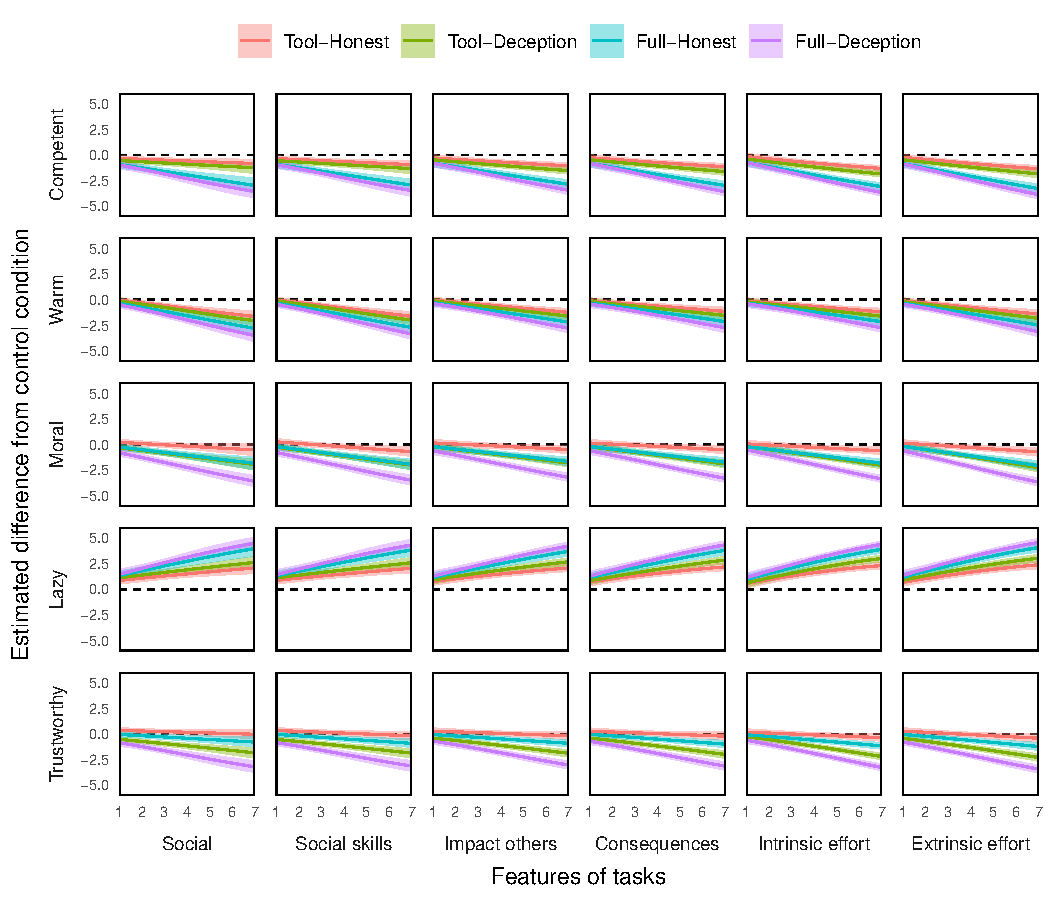
\includegraphics[keepaspectratio]{manuscript_files/figure-pdf/unnamed-chunk-9-1.pdf}}

}

\end{suppfig}%

\newpage

\begin{suppfig}[H]

\caption{\label{suppfig-interaction-pars-study1}Interaction parameters
from models including task-specific features as moderators of the causal
effects of AI outsourcing compared to the control condition in Study 1.
Points and line ranges represent posterior medians and 95\% credible
intervals, respectively.}

\centering{

\pandocbounded{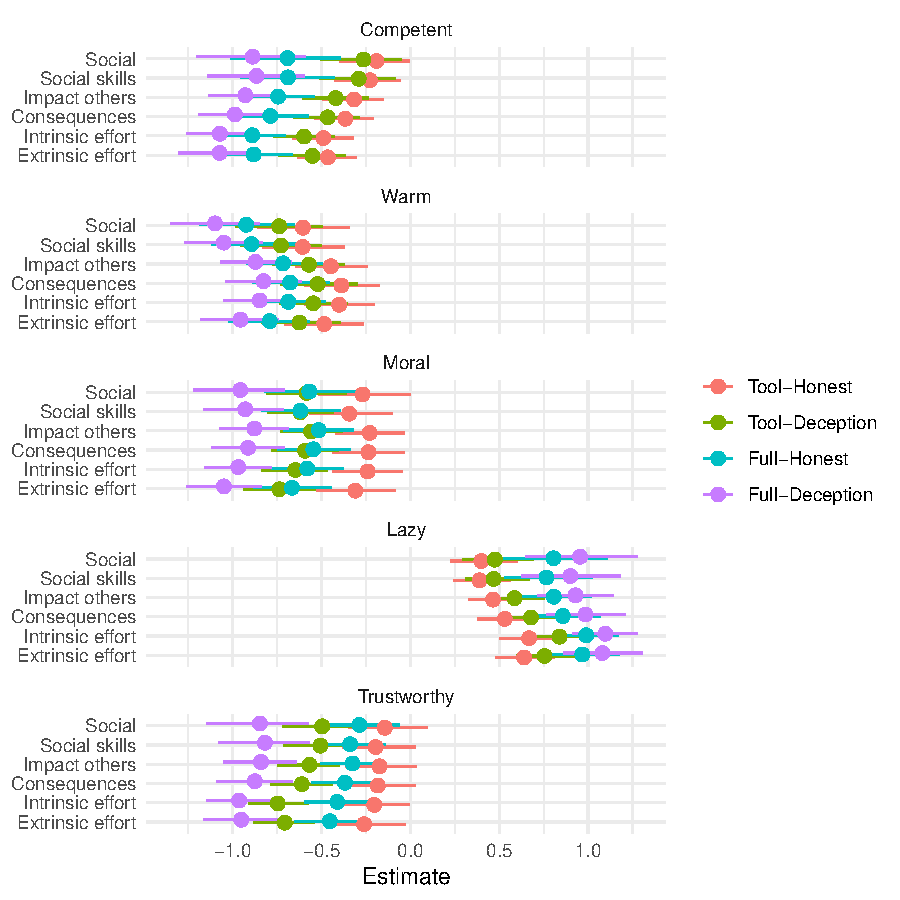
\includegraphics[keepaspectratio]{manuscript_files/figure-pdf/unnamed-chunk-10-1.pdf}}

}

\end{suppfig}%

\newpage

\begin{suppfig}[H]

\caption{\label{suppfig-treatments-person-study2}Character evaluations
in Study 2. Participants in the control condition, the tool outsourcing
condition, and the full outsourcing condition evaluated the ``other
participant'' on (a) competence, (b) warmth, (c) morality, (d) laziness,
and (e) trustworthiness. Jittered points represent participant responses
to the questions, split by whether the writing task was a non-social
task (red) or a social task (blue). Point ranges are estimated marginal
means from the fitted model, pooling over essay answers. Points and line
ranges represent posterior medians and 95\% credible intervals,
respectively.}

\centering{

\pandocbounded{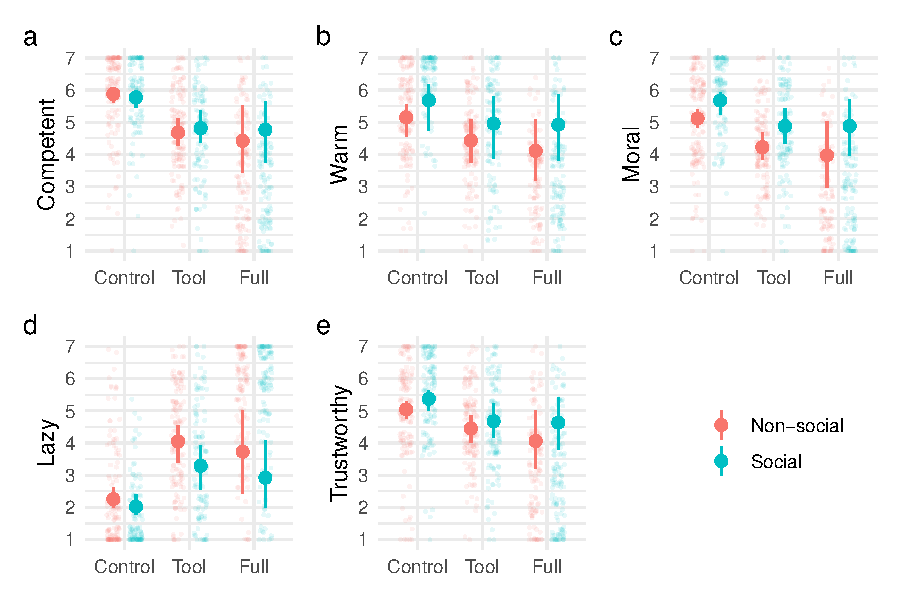
\includegraphics[keepaspectratio]{manuscript_files/figure-pdf/unnamed-chunk-11-1.pdf}}

}

\end{suppfig}%

\newpage

\begin{suppfig}[H]

\caption{\label{suppfig-interactions-study3}The impact of task-specific
features (e.g., being a social task) on the causal effects of
outsourcing to AI compared to the control condition in Study 3. The
y-axis reflects the estimated differences between the experimental
conditions and the control condition (dashed line) on a 7-point Likert
scale. Lines and shaded areas represent posterior medians and 95\%
credible intervals, respectively. The patterns indicate, for example,
more negative effects of outsourcing on character evaluations for tasks
that are rated as more social.}

\centering{

\pandocbounded{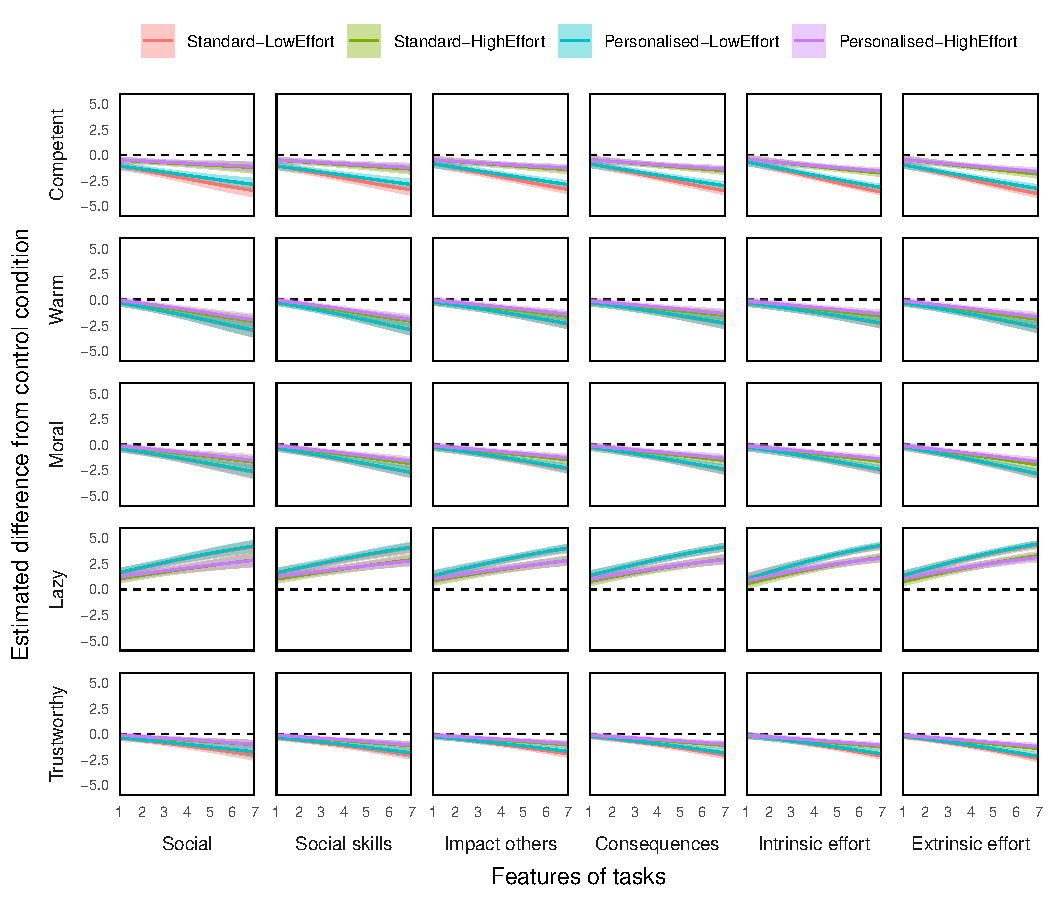
\includegraphics[keepaspectratio]{manuscript_files/figure-pdf/unnamed-chunk-12-1.pdf}}

}

\end{suppfig}%

\newpage

\begin{suppfig}[H]

\caption{\label{suppfig-interaction-pars-study3}Interaction parameters
from models including task-specific features as moderators of the causal
effects of AI outsourcing compared to the control condition in Study 3.
Points and line ranges represent posterior medians and 95\% credible
intervals, respectively.}

\centering{

\pandocbounded{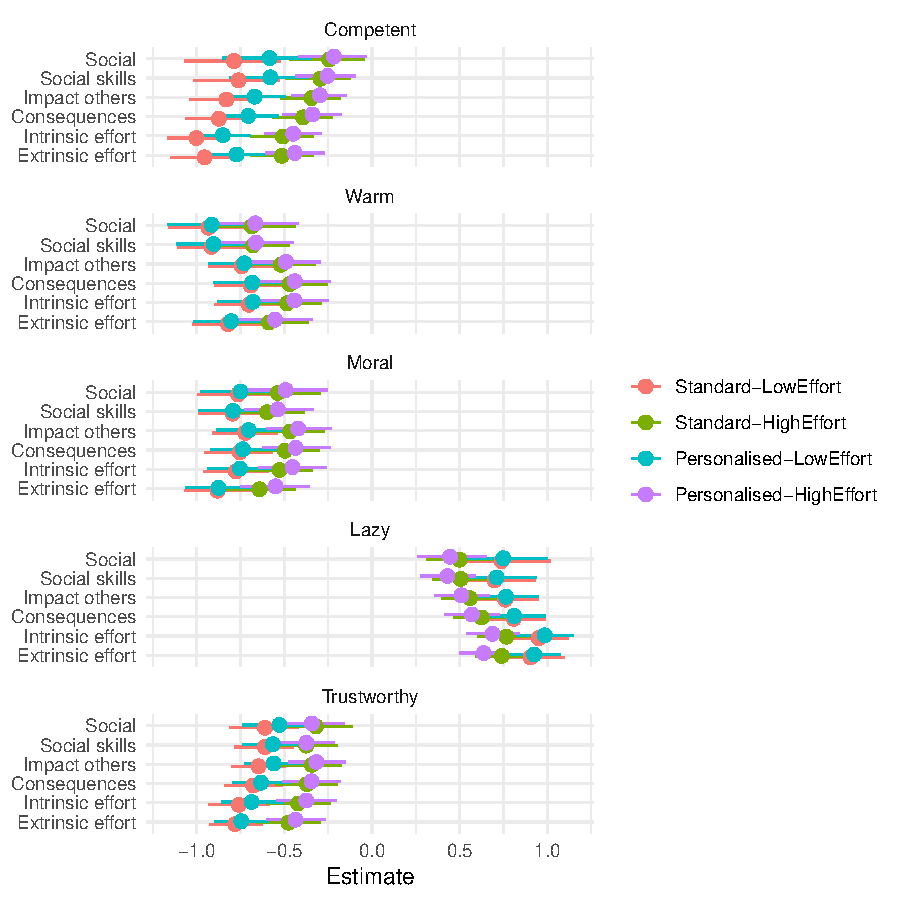
\includegraphics[keepaspectratio]{manuscript_files/figure-pdf/unnamed-chunk-13-1.pdf}}

}

\end{suppfig}%

\newpage

\begin{suppfig}[H]

\caption{\label{suppfig-interactions-study4}The impact of task-specific
features (e.g., being a social task) on the causal effects of
outsourcing to AI compared to the control condition in Study 4. The
y-axis reflects the estimated differences between the experimental
conditions and the control condition (dashed line) on a 7-point Likert
scale. Lines and shaded areas represent posterior medians and 95\%
credible intervals, respectively. The patterns indicate, for example,
more negative effects of outsourcing on character evaluations for tasks
that are rated as more social.}

\centering{

\pandocbounded{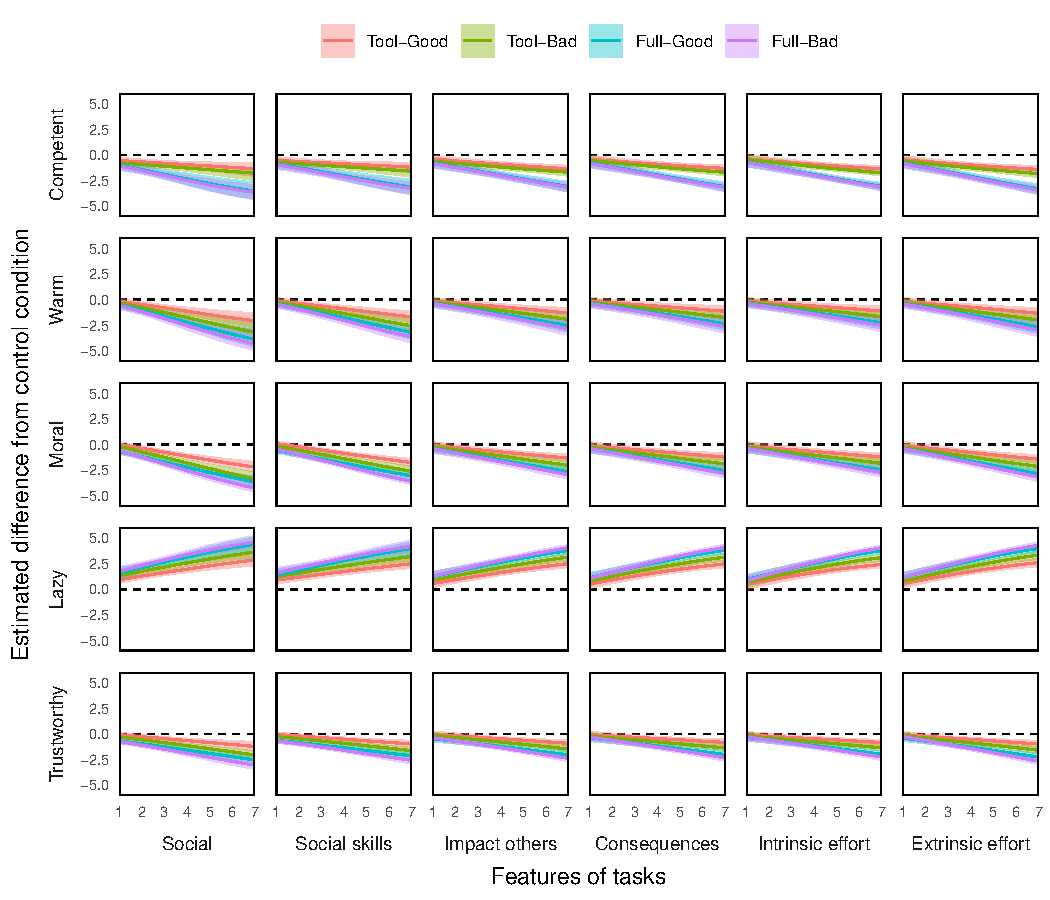
\includegraphics[keepaspectratio]{manuscript_files/figure-pdf/unnamed-chunk-14-1.pdf}}

}

\end{suppfig}%

\newpage

\begin{suppfig}[H]

\caption{\label{suppfig-interaction-pars-study4}Interaction parameters
from models including task-specific features as moderators of the causal
effects of AI outsourcing compared to the control condition in Study 4.
Points and line ranges represent posterior medians and 95\% credible
intervals, respectively.}

\centering{

\pandocbounded{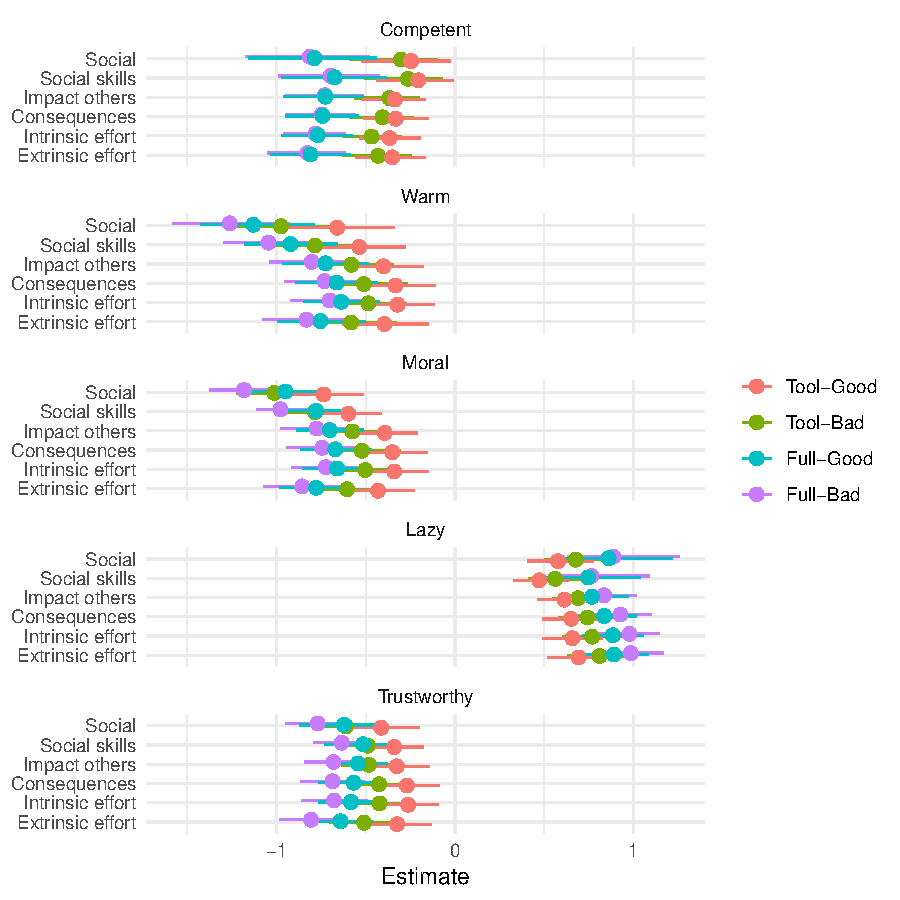
\includegraphics[keepaspectratio]{manuscript_files/figure-pdf/unnamed-chunk-15-1.pdf}}

}

\end{suppfig}%

\newpage

\begin{landscape}

\begin{suppfig}[H]

\caption{\label{suppfig-reasons-tasks-study4}Variation in the effect of
reasons across tasks in Study 4. Tasks are ordered from most social
(top) to least social (bottom) according to ratings from a pilot study.
Point ranges are differences in marginal means on a 7-point Likert scale
between the ``bad reason'' and ``good reason'' conditions, split by
outsourcing type. Points and ranges represent posterior medians and 95\%
credible intervals, respectively.}

\centering{

\pandocbounded{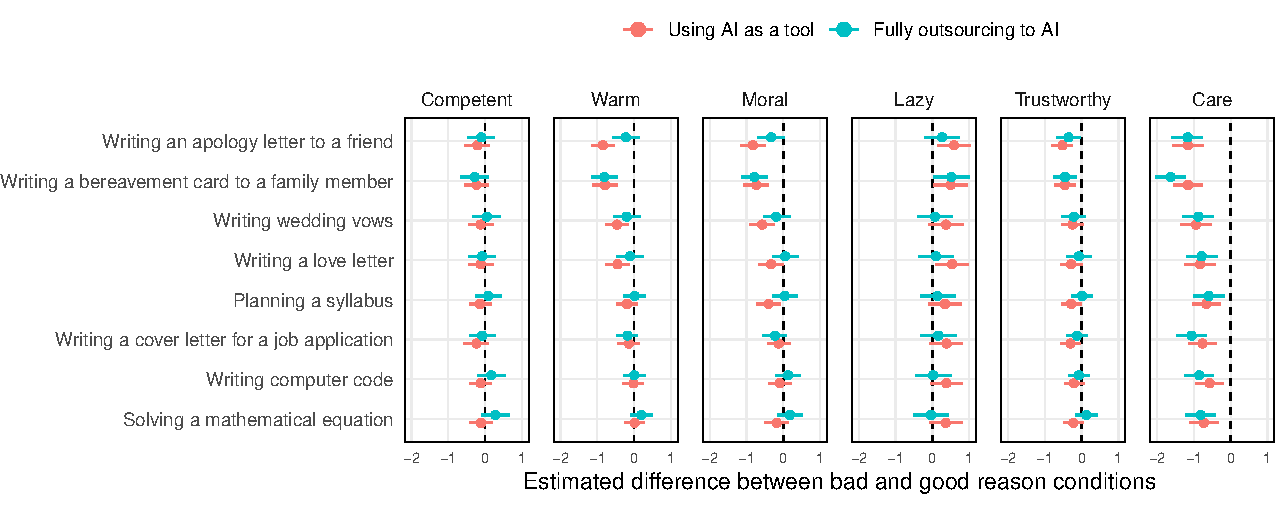
\includegraphics[keepaspectratio]{manuscript_files/figure-pdf/unnamed-chunk-16-1.pdf}}

}

\end{suppfig}%

\end{landscape}

\newpage

\begin{suppfig}[H]

\caption{\label{suppfig-tasks-correlations}Model-estimated task-specific
correlations between all six questions in the first pilot study. Values
are posterior median correlations. A positive correlation indicates that
tasks that are rated highly on one question tend to be rated highly on
another question.}

\centering{

\pandocbounded{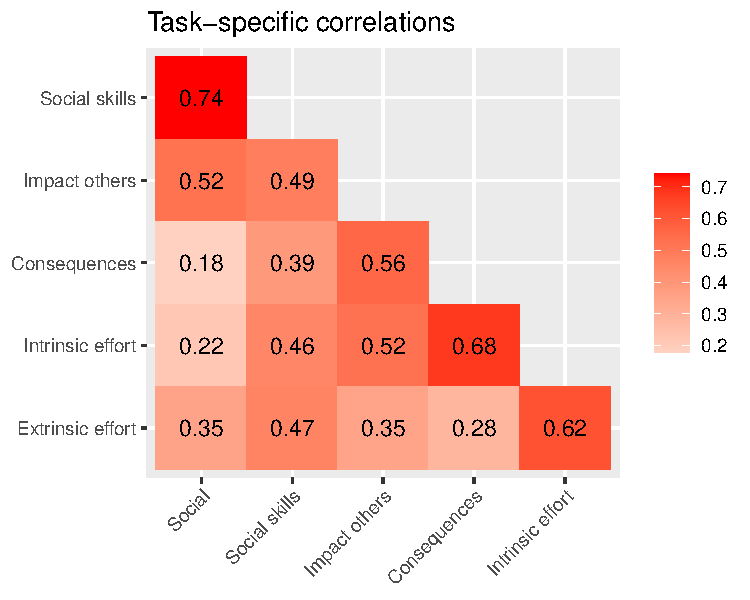
\includegraphics[keepaspectratio]{manuscript_files/figure-pdf/unnamed-chunk-17-1.pdf}}

}

\end{suppfig}%

\newpage

\begin{suppfig}[H]

\caption{\label{suppfig-tasks-social}Model-estimated means for the
question ``Is this a social task?'' across all 20 tasks in the first
pilot study. Grey points represent participant responses to the
question, jittered for easier viewing. Black points are estimated means
from the fitted model, pooling over participants. Black points and line
ranges represent posterior medians and 95\% credible intervals,
respectively.}

\centering{

\pandocbounded{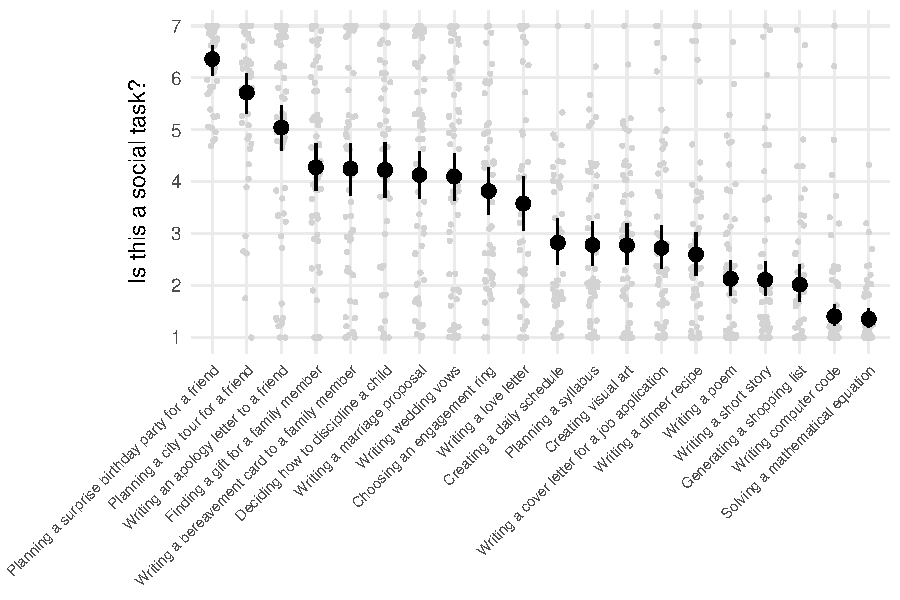
\includegraphics[keepaspectratio]{manuscript_files/figure-pdf/unnamed-chunk-18-1.pdf}}

}

\end{suppfig}%

\newpage

\begin{suppfig}[H]

\caption{\label{suppfig-tasks-socialskills}Model-estimated means for the
question ``Does this task require social skills?'' across all 20 tasks
in the first pilot study. Grey points represent participant responses to
the question, jittered for easier viewing. Black points are estimated
means from the fitted model, pooling over participants. Black points and
line ranges represent posterior medians and 95\% credible intervals,
respectively.}

\centering{

\pandocbounded{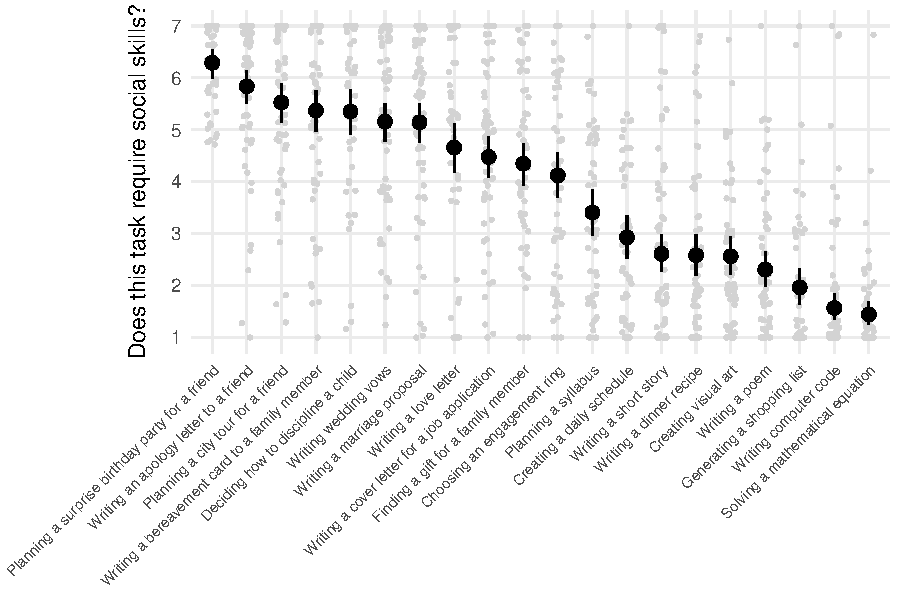
\includegraphics[keepaspectratio]{manuscript_files/figure-pdf/unnamed-chunk-19-1.pdf}}

}

\end{suppfig}%

\newpage

\begin{suppfig}[H]

\caption{\label{suppfig-tasks-impactothers}Model-estimated means for the
question ``Does this task impact other people?'' across all 20 tasks in
the first pilot study. Grey points represent participant responses to
the question, jittered for easier viewing. Black points are estimated
means from the fitted model, pooling over participants. Black points and
line ranges represent posterior medians and 95\% credible intervals,
respectively.}

\centering{

\pandocbounded{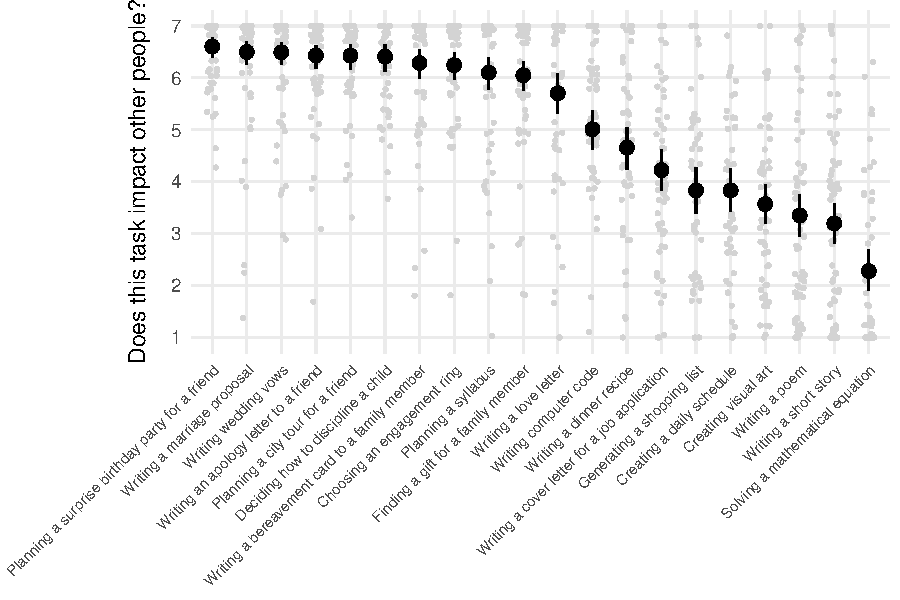
\includegraphics[keepaspectratio]{manuscript_files/figure-pdf/unnamed-chunk-20-1.pdf}}

}

\end{suppfig}%

\newpage

\begin{suppfig}[H]

\caption{\label{suppfig-tasks-consequences}Model-estimated means for the
question ``How important are the consequences of this task?'' across all
20 tasks in the first pilot study. Grey points represent participant
responses to the question, jittered for easier viewing. Black points are
estimated means from the fitted model, pooling over participants. Black
points and line ranges represent posterior medians and 95\% credible
intervals, respectively.}

\centering{

\pandocbounded{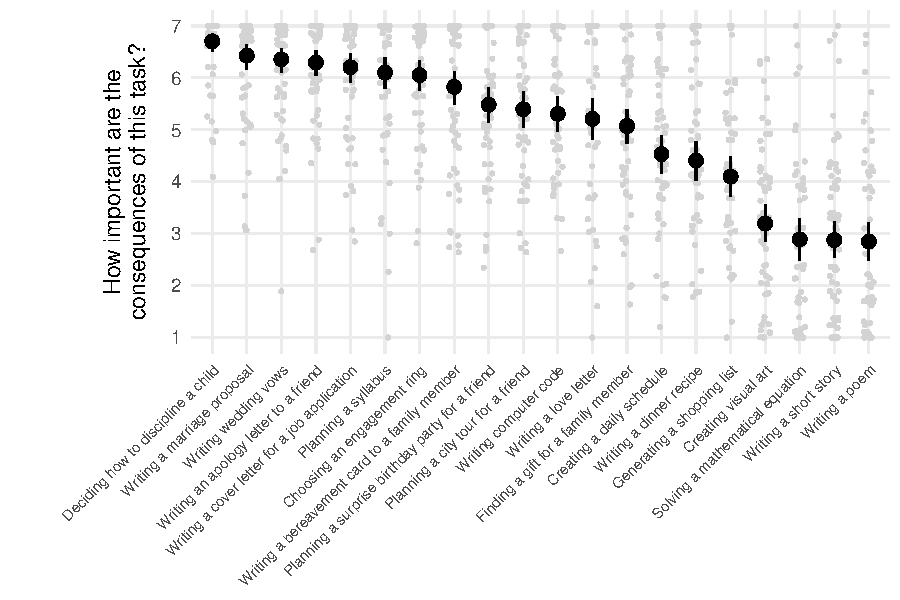
\includegraphics[keepaspectratio]{manuscript_files/figure-pdf/unnamed-chunk-21-1.pdf}}

}

\end{suppfig}%

\newpage

\begin{suppfig}[H]

\caption{\label{suppfig-tasks-intrinsiceffort}Model-estimated means for
the question ``How important is it that effort goes into this task?''
across all 20 tasks in the first pilot study. Grey points represent
participant responses to the question, jittered for easier viewing.
Black points are estimated means from the fitted model, pooling over
participants. Black points and line ranges represent posterior medians
and 95\% credible intervals, respectively.}

\centering{

\pandocbounded{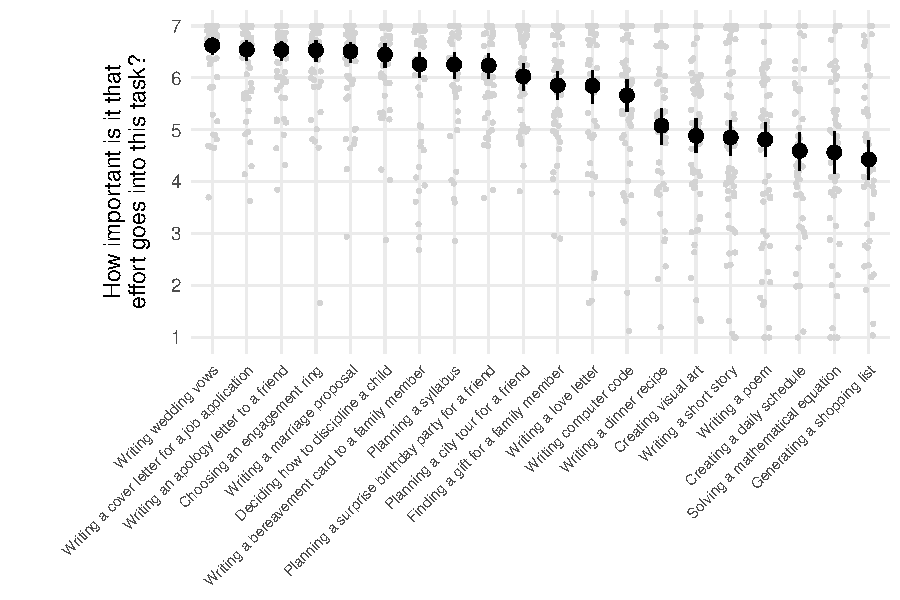
\includegraphics[keepaspectratio]{manuscript_files/figure-pdf/unnamed-chunk-22-1.pdf}}

}

\end{suppfig}%

\newpage

\begin{suppfig}[H]

\caption{\label{suppfig-tasks-extrinsiceffort}Model-estimated means for
the question ``How important is it that others see the effort that goes
into this task?'' across all 20 tasks in the first pilot study. Grey
points represent participant responses to the question, jittered for
easier viewing. Black points are estimated means from the fitted model,
pooling over participants. Black points and line ranges represent
posterior medians and 95\% credible intervals, respectively.}

\centering{

\pandocbounded{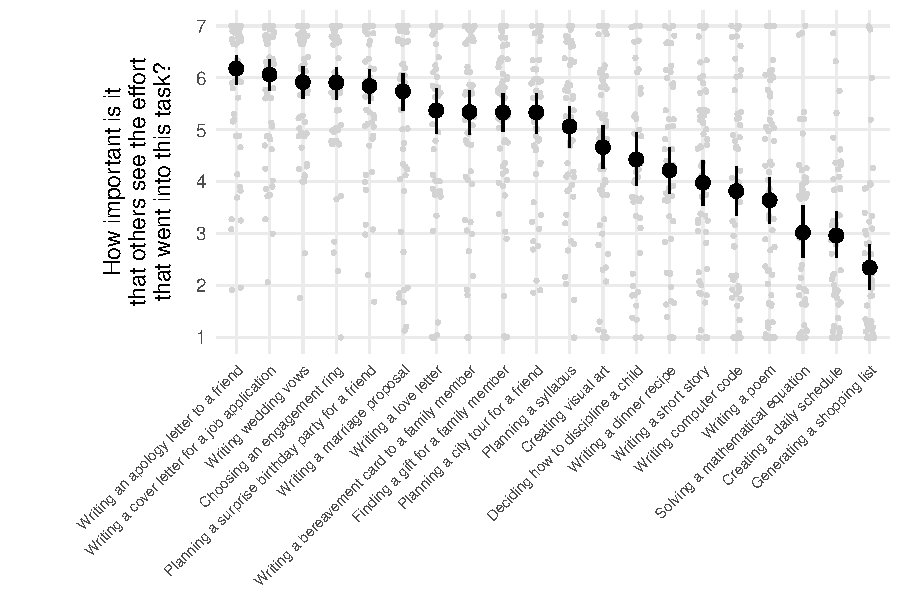
\includegraphics[keepaspectratio]{manuscript_files/figure-pdf/unnamed-chunk-23-1.pdf}}

}

\end{suppfig}%

\newpage

\begin{suppfig}[H]

\caption{\label{suppfig-treatments-pilotstudy2}Character evaluations in
the second pilot study. Participants in the control condition, the AI
outsourcing condition, and the human outsourcing condition evaluated
people in the scenarios on (a) competence, (b) warmth, (c) morality, (d)
laziness, and (e) trustworthiness. Coloured points represent participant
responses to the questions, jittered for easier viewing. Black points
are estimated marginal means from the fitted model, pooling over
participants and tasks. Black points and line ranges represent posterior
medians and 95\% credible intervals, respectively.}

\centering{

\pandocbounded{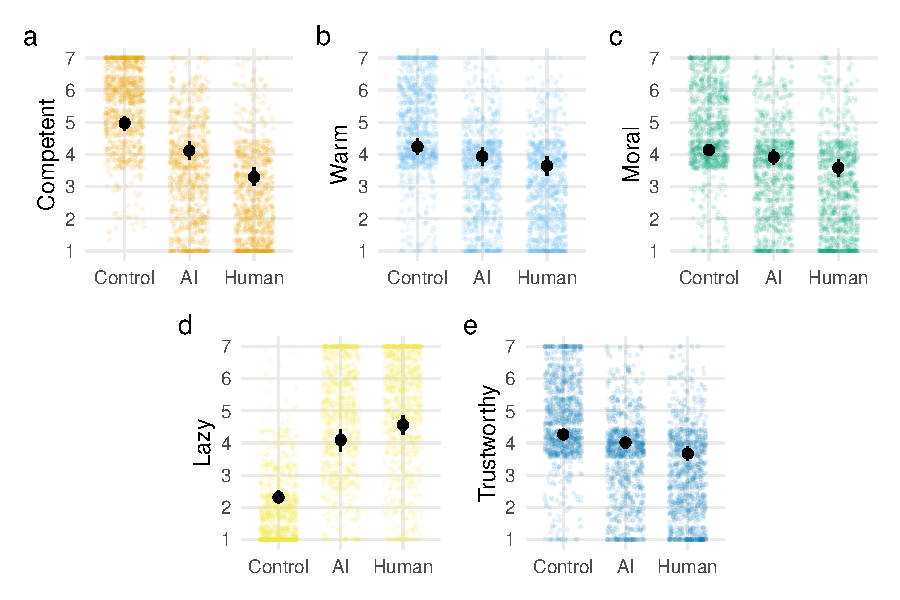
\includegraphics[keepaspectratio]{manuscript_files/figure-pdf/unnamed-chunk-24-1.pdf}}

}

\end{suppfig}%

\newpage

\begin{suppfig}[H]

\caption{\label{suppfig-treatments-by-task-pilotstudy2}Variation in the
effects of outsourcing across tasks in the second pilot study. Tasks are
ordered from most social (top) to least social (bottom) according to
ratings from the first pilot study. Point ranges are differences in
marginal means on a 7-point Likert scale for the AI outsourcing
condition (red) and the human outsourcing condition (blue) compared to
the control condition. Points and ranges represent posterior medians and
95\% credible intervals, respectively.}

\centering{

\pandocbounded{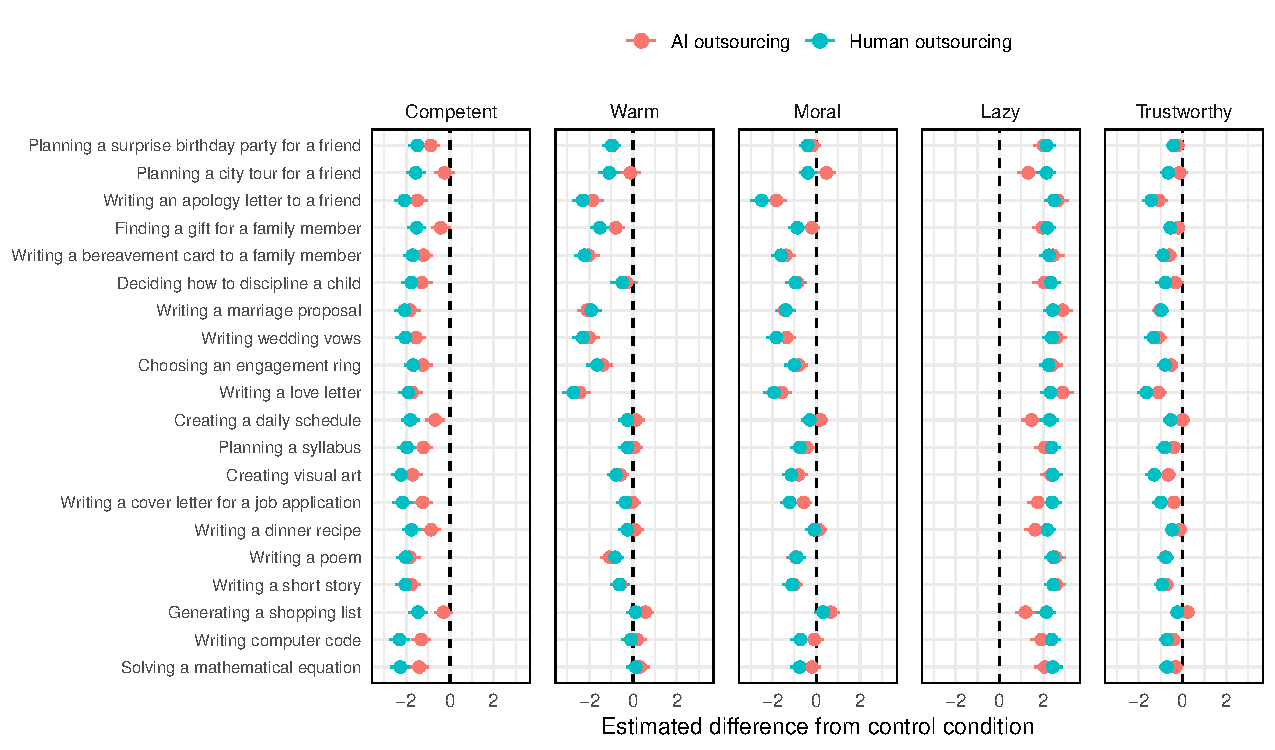
\includegraphics[keepaspectratio]{manuscript_files/figure-pdf/unnamed-chunk-25-1.pdf}}

}

\end{suppfig}%

\newpage

\begin{suppfig}[H]

\caption{\label{suppfig-interactions-pilotstudy2}The impact of
task-specific features (e.g., being a social task) on the causal effects
of outsourcing to AI (red) and humans (blue) compared to the control
condition in the second pilot study. The y-axis reflects the estimated
differences between the experimental conditions and the control
condition (dashed line) on a 7-point Likert scale. Lines and shaded
areas represent posterior medians and 95\% credible intervals,
respectively. The patterns indicate, for example, more negative effects
of outsourcing on character evaluations for tasks that are rated as more
social.}

\centering{

\pandocbounded{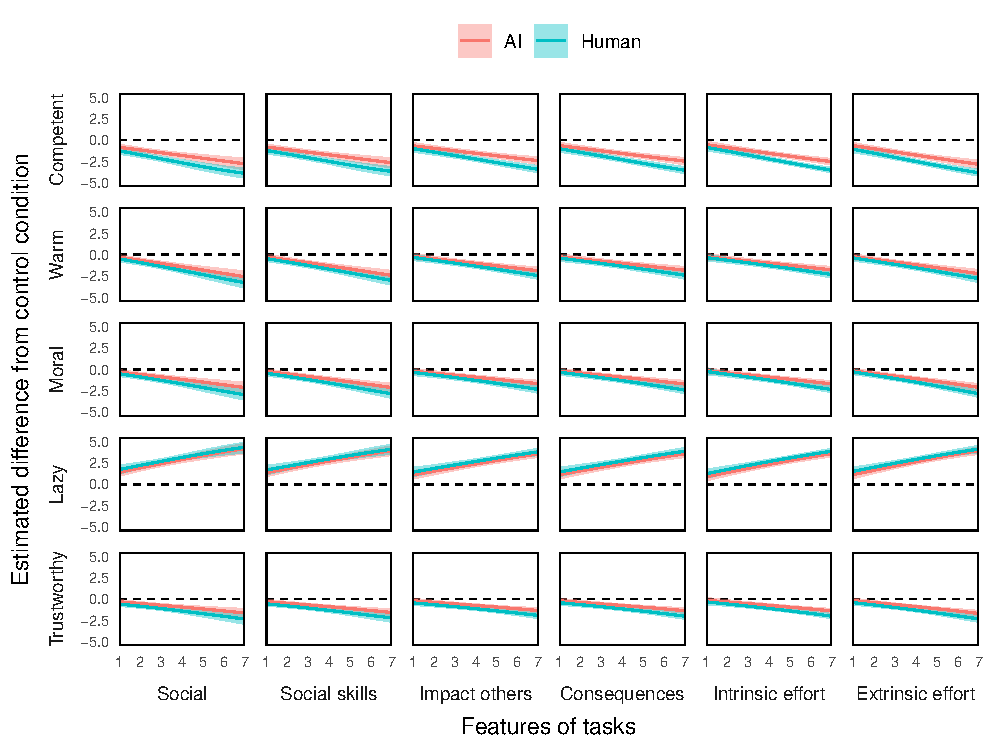
\includegraphics[keepaspectratio]{manuscript_files/figure-pdf/unnamed-chunk-26-1.pdf}}

}

\end{suppfig}%

\newpage

\begin{suppfig}[H]

\caption{\label{suppfig-interaction-pars-pilotstudy2}Interaction
parameters from models including task-specific features as moderators of
the causal effects of AI outsourcing (red) and human outsourcing (blue)
compared to the control condition in the second pilot study. Points and
line ranges represent posterior medians and 95\% credible intervals,
respectively.}

\centering{

\pandocbounded{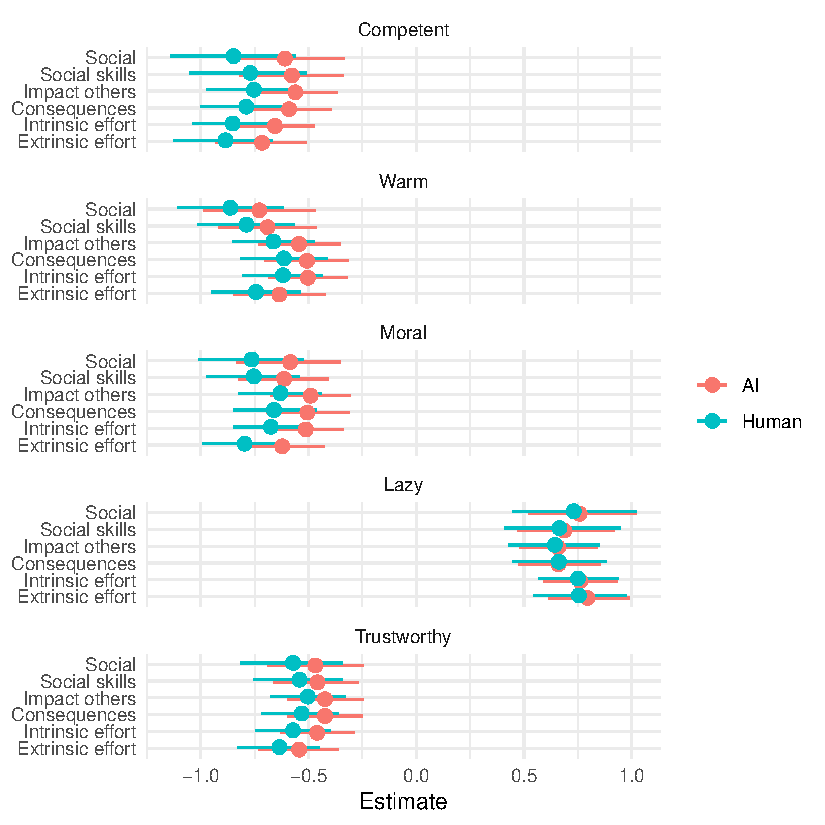
\includegraphics[keepaspectratio]{manuscript_files/figure-pdf/unnamed-chunk-27-1.pdf}}

}

\end{suppfig}%

\newpage

\section{Supplementary Tables}\label{supplementary-tables}

\begin{supptbl}[H]

\caption{\label{supptbl-tasks}Tasks included in the studies.}

\begin{minipage}{\linewidth}

\centering\begingroup\fontsize{10}{12}\selectfont

\begin{tabular}{lccccc}
\toprule
Task & Pilot Study 1 & Pilot Study 2 & Study 1 & Study 2 & Study 4\\
\midrule
Writing wedding vows & $\checkmark$ & $\checkmark$ & $\checkmark$ & $\checkmark$ & $\checkmark$\\
Writing a love letter & $\checkmark$ & $\checkmark$ & $\checkmark$ & $\checkmark$ & $\checkmark$\\
Writing a marriage proposal & $\checkmark$ & $\checkmark$ & $\checkmark$ & $\checkmark$ & \\
Choosing an engagement ring & $\checkmark$ & $\checkmark$ & $\checkmark$ &  & \\
Finding a gift for a family member & $\checkmark$ & $\checkmark$ & $\checkmark$ &  & \\
Deciding how to discipline a child & $\checkmark$ & $\checkmark$ & $\checkmark$ &  & \\
Writing a bereavement card to a family member & $\checkmark$ & $\checkmark$ & $\checkmark$ & $\checkmark$ & $\checkmark$\\
Writing an apology letter to a friend & $\checkmark$ & $\checkmark$ & $\checkmark$ & $\checkmark$ & $\checkmark$\\
Planning a city tour for a friend & $\checkmark$ & $\checkmark$ & $\checkmark$ & $\checkmark$ & \\
Planning a surprise birthday party for a friend & $\checkmark$ & $\checkmark$ & $\checkmark$ & $\checkmark$ & \\
Writing a cover letter for a job application & $\checkmark$ & $\checkmark$ & $\checkmark$ & $\checkmark$ & $\checkmark$\\
Writing computer code & $\checkmark$ & $\checkmark$ & $\checkmark$ & $\checkmark$ & $\checkmark$\\
Solving a mathematical equation & $\checkmark$ & $\checkmark$ & $\checkmark$ & $\checkmark$ & $\checkmark$\\
Planning a syllabus & $\checkmark$ & $\checkmark$ & $\checkmark$ & $\checkmark$ & $\checkmark$\\
Writing a short story & $\checkmark$ & $\checkmark$ & $\checkmark$ & $\checkmark$ & \\
Writing a poem & $\checkmark$ & $\checkmark$ & $\checkmark$ & $\checkmark$ & \\
Creating visual art & $\checkmark$ & $\checkmark$ & $\checkmark$ &  & \\
Creating a daily schedule & $\checkmark$ & $\checkmark$ & $\checkmark$ & $\checkmark$ & \\
Generating a shopping list & $\checkmark$ & $\checkmark$ & $\checkmark$ & $\checkmark$ & \\
Writing a dinner recipe & $\checkmark$ & $\checkmark$ & $\checkmark$ & $\checkmark$ & \\
\bottomrule
\end{tabular}
\endgroup{}

\end{minipage}%

\end{supptbl}%

\newpage

\begin{supptbl}[H]

\caption{\label{supptbl-essay-answers-social-study2}Pre-generated essay
answers to the social prompt in Study 2.}

\begin{minipage}{\linewidth}

\begingroup
\linespread{1}\selectfont
\centering\begingroup\fontsize{10}{12}\selectfont

\begin{tabular}{>{\raggedright\arraybackslash}p{2cm}>{\raggedright\arraybackslash}p{14cm}}
\toprule
Answer & Text\\
\midrule
Father & My dad is one of the most important people in my life. He's always been someone I look up to and rely on. Throughout my whole life, he's been there to guide me, teach me, and support me in everything I do. What makes my dad special is how much he cares about our family. He works hard every day to make sure we have what we need, but no matter how busy he is, he always makes time for us. My dad is emotionally strong. Even though he doesn't show his emotions a lot, I can tell how much he cares by how much he does for us. When things get hard, he stays calm and steady, and that helps me feel better. One of my favorite things about my dad is how much he loves to teach. He knows so much and is always happy to share what he knows. He explains things in a way that makes sense and is easy to understand. I also love my dad's sense of humor. He always knows how to make me laugh with a joke or a funny story. His laughter makes everything feel lighter and happier. My dad has taught me so much about working hard, being kind, and staying strong when life is tough. I'm so thankful for everything he's done for me, and I'm proud to have him as my dad!\\
Sister & My sister is one of the most important people in my life. She is special because she always supports me. She has a way of making me feel confident, even when I'm unsure of myself. Whenever I'm scared to try something new, she's the first to remind me of what I can do. Her belief in me helps me believe in myself. My sister also has a really kind heart. She always thinks about others and does her best to help. She's always putting others first, whether it's being there for a friend or helping out with family. Her kindness is something I look up to and try to follow. Another thing I love about my sister is how funny she is. She has a great sense of humor and always knows how to make people laugh, even in serious moments. If I'm ever feeling down, she can cheer me up with a joke or a funny story. Her laughter makes everything feel lighter and happier. What I admire most about my sister is how strong she is. She's faced tough times but never lets them hold her back. Her strength gives me courage to keep going when life gets hard. My sister is more than just a family member — she's my role model and my rock!\\
Friend & My best friend is one of the most amazing people I know. She's someone I can count on no matter what. What makes her so special is her kindness. She always makes people feel important and cared for. Whether it's helping someone she just met or being there for her friends, she's the first to offer support. She never hesitates to help me, whether I'm upset or just having a bad day. She also has a great sense of humor that can cheer anyone up. She finds ways to laugh about even the smallest things, and her laugh is so contagious! Her laughter makes everything feel lighter and happier. What I admire most about her is how strong she is. Life hasn't always been easy for her, but she never gives up. She stays calm and keeps going, no matter what happens. Watching her face challenges in adulthood has taught me to be brave and not let hard times hold me back. My best friend has shown me what it means to be loyal, caring, and strong. I feel so lucky to have her in my life. I try to be as good of a friend to her as she is to me. She inspires me to be a better person!\\
\bottomrule
\end{tabular}
\endgroup{}
\endgroup

\end{minipage}%

\end{supptbl}%

\newpage

\begin{supptbl}[H]

\caption{\label{supptbl-essay-answers-nonsocial-study2}Pre-generated
essay answers to the non-social prompt in Study 2.}

\begin{minipage}{\linewidth}

\begingroup
\linespread{1}\selectfont
\centering\begingroup\fontsize{10}{12}\selectfont

\begin{tabular}{>{\raggedright\arraybackslash}p{2cm}>{\raggedright\arraybackslash}p{14cm}}
\toprule
Answer & Text\\
\midrule
The Hobbit & I will focus on describing the book “The Hobbit” by Tolkien. The Hobbit is a fantasy adventure story about Bilbo Baggins. Bilbo is a quiet hobbit who lives in the Shire. His life changes when Gandalf the wizard and a company of dwarves ask him to join their quest to take back treasure stolen by a dragon. At the beginning of the journey, Bilbo and the dwarves are nearly eaten by trolls, but Gandalf saves them. Then later, in the Misty Mountains, Bilbo meets a creature called Gollum and finds a magical ring that makes him invisible. This ring later becomes very important in “The Lord of the Rings”. As they travel, the group fights goblins, giant spiders in Mirkwood forest, and they get captured by Wood-elves. Bilbo shows his bravery by saving the group several times. Finally, they reach the Lonely Mountain where the dragon Smaug lives. Bilbo sneaks into the dragon's lair and finds a weak spot in Smaug's armor. The dragon gets angry and attacks the nearby town by a lake. Eventually, Smaug is killed. With the dragon dead, humans, elves, and dwarves all want the treasure. This leads to the “Battle of the Five Armies”. Tolkien doesn't describe the battle in too much detail, but we later learn that the leader of the dwarves Thorin has fought bravely and died from his wounds. At the end of the story, Bilbo returns home to the Shire, richer and wiser from his adventure. He is happy to be back in his quiet life, and sets out to write a book of his adventures - which sets the stage for the sequel, The Lord of the Rings.\\
Buffy the Vampire Slayer & I will focus on describing the TV show “Buffy the Vampire Slayer”. Buffy is a TV show that completely flips the script on traditional high school dramas and supernatural horror. It's about a teenager, Buffy Summers, who's tasked with being the Slayer – basically a chosen one who hunts vampires and other demons. But what sets the show apart is how Buffy struggles to balance her responsibility with the regular teenage experience. She's not just fighting creatures of the night, she's also balancing school and friendships at the same time. One of the most striking things about Buffy is how layered the characters are. Buffy is tough and witty, but she's also vulnerable. She's faced with loss, guilt, and trying to make sense of her life outside of the supernatural chaos. And then there's her team. Willow is the nerdy, sweet heart of the group, Xander is the funny loyal friend, and Giles (Buffy's Watcher) is the stern mentor who's also loving. Each character feels real, with their own flaws and growth arcs. The show has this incredible ability to mix humor, heart, and horror seamlessly. The dialogue is sharp and full of clever pop culture references. Yet, the writing isn't afraid to get serious, exploring themes like trauma and growing up. The monsters Buffy faces often mirror real-life challenges, making the stakes feel personal. I love Buffy. It's a show that's smart and emotional, blending witty banter with moments of real depth. It's got a cult following for a reason!\\
Titanic & I will focus on describing the film “Titanic”. The genre is a mix of romance, disaster, and historical tragedy. The film tells the love story of Jack and Rose, two passengers from different social classes aboard the passenger ship Titanic. Jack is a poor artist, but he manages to win a ticket to the ship's maiden voyage. Rose is a young upper-class woman who is feeling trapped in her engagement to her fiance. Jack and Rose cross paths on the ship, and they fall in love. The film balances the spectacle of the ship's design and atmosphere with the tension that gradually builds as the audience knows what fate awaits. The Titanic sails into the icy waters of the Atlantic and strikes an iceberg. Chaos immediately erupts. The film allows viewers to experience the terror, confusion, and heartbreak of the tragedy, showcasing both personal stories and the broader catastrophe. At its core, the film is a romance. But Titanic also touches on themes of class and fate. It highlights the disparity between the elite and the working-class passengers who are doomed to different fates. The film also explores the sense of inevitability that comes with knowing the ship's doom. The most iconic scene from the film is arguably the scene where Jack and Rose stand together at the bow, arms outstretched. They seem free, but the scene also foreshadows the devastating crash to come. The film is truly heartbreaking!\\
\bottomrule
\end{tabular}
\endgroup{}
\endgroup

\end{minipage}%

\end{supptbl}%

\newpage

\begin{supptbl}[H]

\caption{\label{supptbl-essay-comprehension-study2}Reading times and
comprehension rates for the essay answers in Study 2. Expected reading
times were calculated based on an estimated reading speed of 275 words
per minute. Comprehension rates are the percentage of participants who
answered the comprehension question correctly.}

\begin{minipage}{\linewidth}

\centering\begingroup\fontsize{9}{11}\selectfont

\begin{tabular}{llrrrr}
\toprule
Prompt & Answer & Number of words & Expected reading time (secs) & Average reading time (secs) & Comprehension (\%)\\
\midrule
Social & Father & 234 & 51.05 & 47.25 & 100.00\\
 & Friend & 211 & 46.04 & 49.91 & 98.50\\
 & Sister & 218 & 47.56 & 50.25 & 99.21\\
Non-social & Buffy & 251 & 54.76 & 62.46 & 100.00\\
 & Hobbit & 278 & 60.65 & 65.97 & 99.28\\
 & Titanic & 239 & 52.15 & 63.90 & 100.00\\
\bottomrule
\end{tabular}
\endgroup{}

\end{minipage}%

\end{supptbl}%

\newpage

\begin{supptbl}[H]

\caption{\label{supptbl-manipulation-check-study2}Percentage of
participants in Study 2 who passed the manipulation check and reported
that they believed the manipulation, split by condition.}

\begin{minipage}{\linewidth}

\centering\begingroup\fontsize{11}{13}\selectfont

\begin{tabular}{lrr}
\toprule
Condition & Pass manipulation check (\%) & Believe manipulation (\%)\\
\midrule
Control & 98.10 & 71.10\\
Tool outsourcing & 96.11 & 77.99\\
Full outsourcing & 100.00 & 86.07\\
\bottomrule
\end{tabular}
\endgroup{}

\end{minipage}%

\end{supptbl}%

\newpage

\begin{supptbl}[H]

\caption{\label{supptbl-treatment-diffs-person-study2}Pairwise contrasts
for character evaluations in Study 2. Numbers reflect differences in
marginal means on a 7-point Likert scale. Estimates are pooled over
essay answers. The bottom rows represent the interactions between
outsourcing type and task type. Main numbers are posterior medians,
numbers in the square brackets are 95\% credible intervals.}

\begin{minipage}{\linewidth}

\centering\begingroup\fontsize{7.5}{9.5}\selectfont

\begin{tabular}{llllll}
\toprule
\multicolumn{1}{c}{ } & \multicolumn{5}{c}{Response} \\
\cmidrule(l{3pt}r{3pt}){2-6}
  & Competent & Warm & Moral & Lazy & Trustworthy\\
\midrule
\addlinespace[0.3em]
\multicolumn{6}{l}{\textbf{Effect of outsourcing type}}\\
\addlinespace[0.3em]
\multicolumn{6}{l}{\textbf{  Task type = Social}}\\
\hspace{1em}Tool Social - Control Social & -0.97 [-1.33 -0.45] & -0.74 [-1.25 -0.12] & -0.81 [-1.16 -0.30] & 1.31 [0.59 1.76] & -0.71 [-1.07 -0.21]\\
\hspace{1em}Full Social - Control Social & -0.99 [-1.96 -0.17] & -0.75 [-1.55 -0.03] & -0.78 [-1.63 -0.04] & 0.87 [0.05 1.96] & -0.73 [-1.50 0.00]\\
\hspace{1em}Full Social - Tool Social & -0.03 [-1.13 0.92] & -0.03 [-1.06 0.92] & 0.01 [-0.95 0.87] & -0.41 [-1.38 0.84] & -0.03 [-0.91 0.77]\\
\addlinespace[0.3em]
\multicolumn{6}{l}{\textbf{  Task type = Non-social}}\\
\hspace{1em}Tool Non-social - Control Non-social & -1.21 [-1.55 -0.76] & -0.74 [-1.23 -0.10] & -0.91 [-1.28 -0.42] & 1.82 [1.13 2.26] & -0.60 [-0.98 -0.17]\\
\hspace{1em}Full Non-social - Control Non-social & -1.48 [-2.41 -0.37] & -1.07 [-1.89 -0.11] & -1.15 [-2.11 -0.11] & 1.48 [0.21 2.75] & -1.00 [-1.81 -0.04]\\
\hspace{1em}Full Non-social - Tool Non-social & -0.28 [-1.30 0.91] & -0.33 [-1.31 0.72] & -0.25 [-1.28 0.86] & -0.31 [-1.73 1.03] & -0.40 [-1.28 0.62]\\
\addlinespace[0.3em]
\multicolumn{6}{l}{\textbf{Effect of task type}}\\
\hspace{1em}Control Social - Control Non-social & -0.11 [-0.39 0.17] & 0.57 [-0.16 0.99] & 0.57 [0.15 0.88] & -0.24 [-0.55 0.11] & 0.33 [-0.02 0.65]\\
\hspace{1em}Tool Social - Tool Non-social & 0.13 [-0.30 0.61] & 0.55 [-0.37 1.32] & 0.66 [0.11 1.15] & -0.76 [-1.35 -0.15] & 0.22 [-0.28 0.76]\\
\hspace{1em}Full Social - Full Non-social & 0.34 [-0.37 1.07] & 0.83 [-0.16 1.68] & 0.92 [0.13 1.68] & -0.82 [-1.72 0.12] & 0.56 [-0.14 1.27]\\
\addlinespace[0.3em]
\multicolumn{6}{l}{\textbf{Interaction effect}}\\
\hspace{1em}Interaction: Tool - Control & 0.24 [-0.18 0.69] & -0.01 [-0.52 0.59] & 0.10 [-0.32 0.57] & -0.52 [-1.06 0.00] & -0.11 [-0.53 0.38]\\
\hspace{1em}Interaction: Full - Control & 0.46 [-0.21 1.13] & 0.29 [-0.37 0.94] & 0.35 [-0.33 1.05] & -0.57 [-1.41 0.28] & 0.24 [-0.41 0.90]\\
\hspace{1em}Interaction: Full - Tool & 0.21 [-0.60 1.02] & 0.29 [-0.58 1.14] & 0.25 [-0.53 1.09] & -0.06 [-1.03 0.99] & 0.35 [-0.42 1.14]\\
\bottomrule
\end{tabular}
\endgroup{}

\end{minipage}%

\end{supptbl}%

\newpage

\begin{landscape}

\begin{supptbl}[H]

\caption{\label{supptbl-text-analysis-study5}Pairwise comparisons of
word frequencies between conditions. LL = log likelihood.}

\begin{minipage}{\linewidth}

\centering\begingroup\fontsize{8}{10}\selectfont

\begin{tabular}{lrrrrrrrrr}
\toprule
Word & Control
Freq. & Tool
Freq. & Full
Freq. & \%DIFF
Full vs Control & LL
Full vs Control & \%DIFF
Tool vs Control & LL
Tool vs Control & \%DIFF
Full vs Tool & LL
Full vs Tool\\
\midrule
Lazy & 0 & 46 & 82 & 14138.18 & 97.16 & 6061.29 & 42.55 & 131.09 & 21.76\\
Genuine & 36 & 11 & 12 & -71.06 & 16.19 & -79.54 & 25.91 & 41.42 & 0.69\\
Loves & 9 & 9 & 0 & -95.18 & 10.50 & -33.03 & 0.72 & -92.80 & 7.21\\
Romantic & 0 & 7 & 0 & -13.18 & 0.00 & 837.59 & 4.42 & -90.74 & 5.16\\
Thoughtful & 13 & 0 & 0 & -96.66 & 16.27 & -97.42 & 19.99 & 29.64 & 0.02\\
Caring & 35 & 12 & 0 & -98.76 & 49.01 & -77.04 & 22.85 & -94.60 & 10.36\\
\bottomrule
\end{tabular}
\endgroup{}

\end{minipage}%

\end{supptbl}%

\end{landscape}

\newpage

\begin{supptbl}[H]

\caption{\label{supptbl-treatment-diffs-pilotstudy2}Pairwise contrasts
in the second pilot study. Numbers reflect differences in marginal means
on a 7-point Likert scale, pooling over participants and tasks. Main
numbers are posterior medians, numbers in the square brackets are 95\%
credible intervals.}

\begin{minipage}{\linewidth}

\centering\begingroup\fontsize{9}{11}\selectfont

\begin{tabular}{llllll}
\toprule
\multicolumn{1}{c}{ } & \multicolumn{5}{c}{Response} \\
\cmidrule(l{3pt}r{3pt}){2-6}
  & Competent & Warm & Moral & Lazy & Trustworthy\\
\midrule
AI - Control & -0.86 [-1.14 -0.56] & -0.30 [-0.57 -0.03] & -0.22 [-0.46 0.02] & 1.78 [1.42 2.13] & -0.25 [-0.44 -0.06]\\
Human - Control & -1.68 [-1.97 -1.36] & -0.59 [-0.88 -0.29] & -0.55 [-0.81 -0.28] & 2.25 [1.90 2.59] & -0.59 [-0.82 -0.37]\\
Human - AI & -0.82 [-1.16 -0.47] & -0.29 [-0.61 0.04] & -0.33 [-0.63 -0.03] & 0.46 [0.07 0.89] & -0.34 [-0.59 -0.09]\\
\bottomrule
\end{tabular}
\endgroup{}

\end{minipage}%

\end{supptbl}%

\newpage

\section{Supplementary References}\label{supplementary-references}

\setlength{\parindent}{-20pt}
\setlength{\leftskip}{20pt}

Boyd, R. L. (2019). BUTTER: Basic unit-transposable text experimentation
resource. Available from \url{https://www.butter.tools/}

Gregson, R., Piazza, J., \& Boyd, R. L. (2022). `Against the cult of
veganism': Unpacking the social psychology and ideology of anti-vegans.
\emph{Appetite}, \emph{178}, 106143.
doi:\href{https://doi.org/10.1016/j.appet.2022.106143}{10.1016/j.appet.2022.106143}

Rayson, P., \& Garside, R. (2000). Comparing corpora using frequency
profiling. \emph{Proceedings of the Workshop on Comparing Corpora -
Volume 9}, 1--6. Presented in Hong Kong.
doi:\href{https://doi.org/10.3115/1117729.1117730}{10.3115/1117729.1117730}






\end{document}
